\section{Summary statistics}
\label{sec:summary-statistics}

\subsection{Partial correlation coefficient}
\label{subsec:partial-correlation-coefficient}

The correlation coefficient $\rho_{\traiti, \traitj}$ give the total regression between two variables.
Partial-correlation coefficient account for the entire covariance matrix, and measure the correlation between $2$ traits, knowing the values of all the other traits:
\begin{equation}
    \rho_{\traiti, \traitj | c \in \traitInterval \setminus \{ a, b\} } = - \dfrac{\Precisionmatrix_{\traiti, \traitj}}{\sqrt{\Precisionmatrix_{\traiti, \traiti} \Precisionmatrix_{\traitj, \traitj}}},
\end{equation}
where the precision matrix $\PrecisionMatrix$ is the inverse of the covariance matrix:
\begin{equation}
    \PrecisionMatrix = \CovarianceMatrix^{-1}
\end{equation}

\subsection{Fitness profile entropy}
\label{subsec:fitness-profile-entropy}

For a category $\cat$, the Shannon entropy ($\entropy$) of the fitness profile is defined as:
\begin{equation}
    \entropy\catexp = - \sum\limits_{\aSetAa} \base\catexp_{\aminoacid} \log \left( \base\catexp_{\aminoacid} \right)
\end{equation}
The Shannon entropy measures the flatness of the fitness profile, with a value of $0$ corresponding to a single peak fitness landscape (only one amino acid is present), and a value of $log(20)\simeq3$ corresponding to a neutral landscape, where each amino acid has the same fitness.

The Shannon entropy can be averaged over all sites as:
\begin{equation}
    \langle \entropy \rangle = \dfrac{1}{\Nsite}\sum\limits_{\Setsite} \entropy^{\catsite}
\end{equation}


\section{Simulations}
\label{sec:supp-mat-simulations}

\subsection{Independent fitness profiles}
Under a simulation with site-independent fitness profiles, a fitness profile give a fitness for each amino acid (vector of size $20$).
Each site of the protein has a specific amino-acid fitness profile.
Overall, the protein fitness is computed as the sum of site-specific fitness, obtained by accessing the amino acid present at each site of the protein.
For each possible mutant, we compute the selection coefficient of the mutant:
\begin{equation}
    s \left( \mathbb{S}^{t},\mathbb{S}^{t+1}\right) = \sum\limits_{1 \leq \site \leq \Nsite} \ln \left( \dfrac{\Base_{\site} \left(\mathbb{S}^{t+1}(\site) \right)}{\Base_{\site} \left(\mathbb{S}^{t}(\site) \right)} \right),
\end{equation}
where $\Base_{\site}$ is the fitness profile at site $\site$, obtained in empirical experiment \citep{Bloom2017}.

\begin{center}
    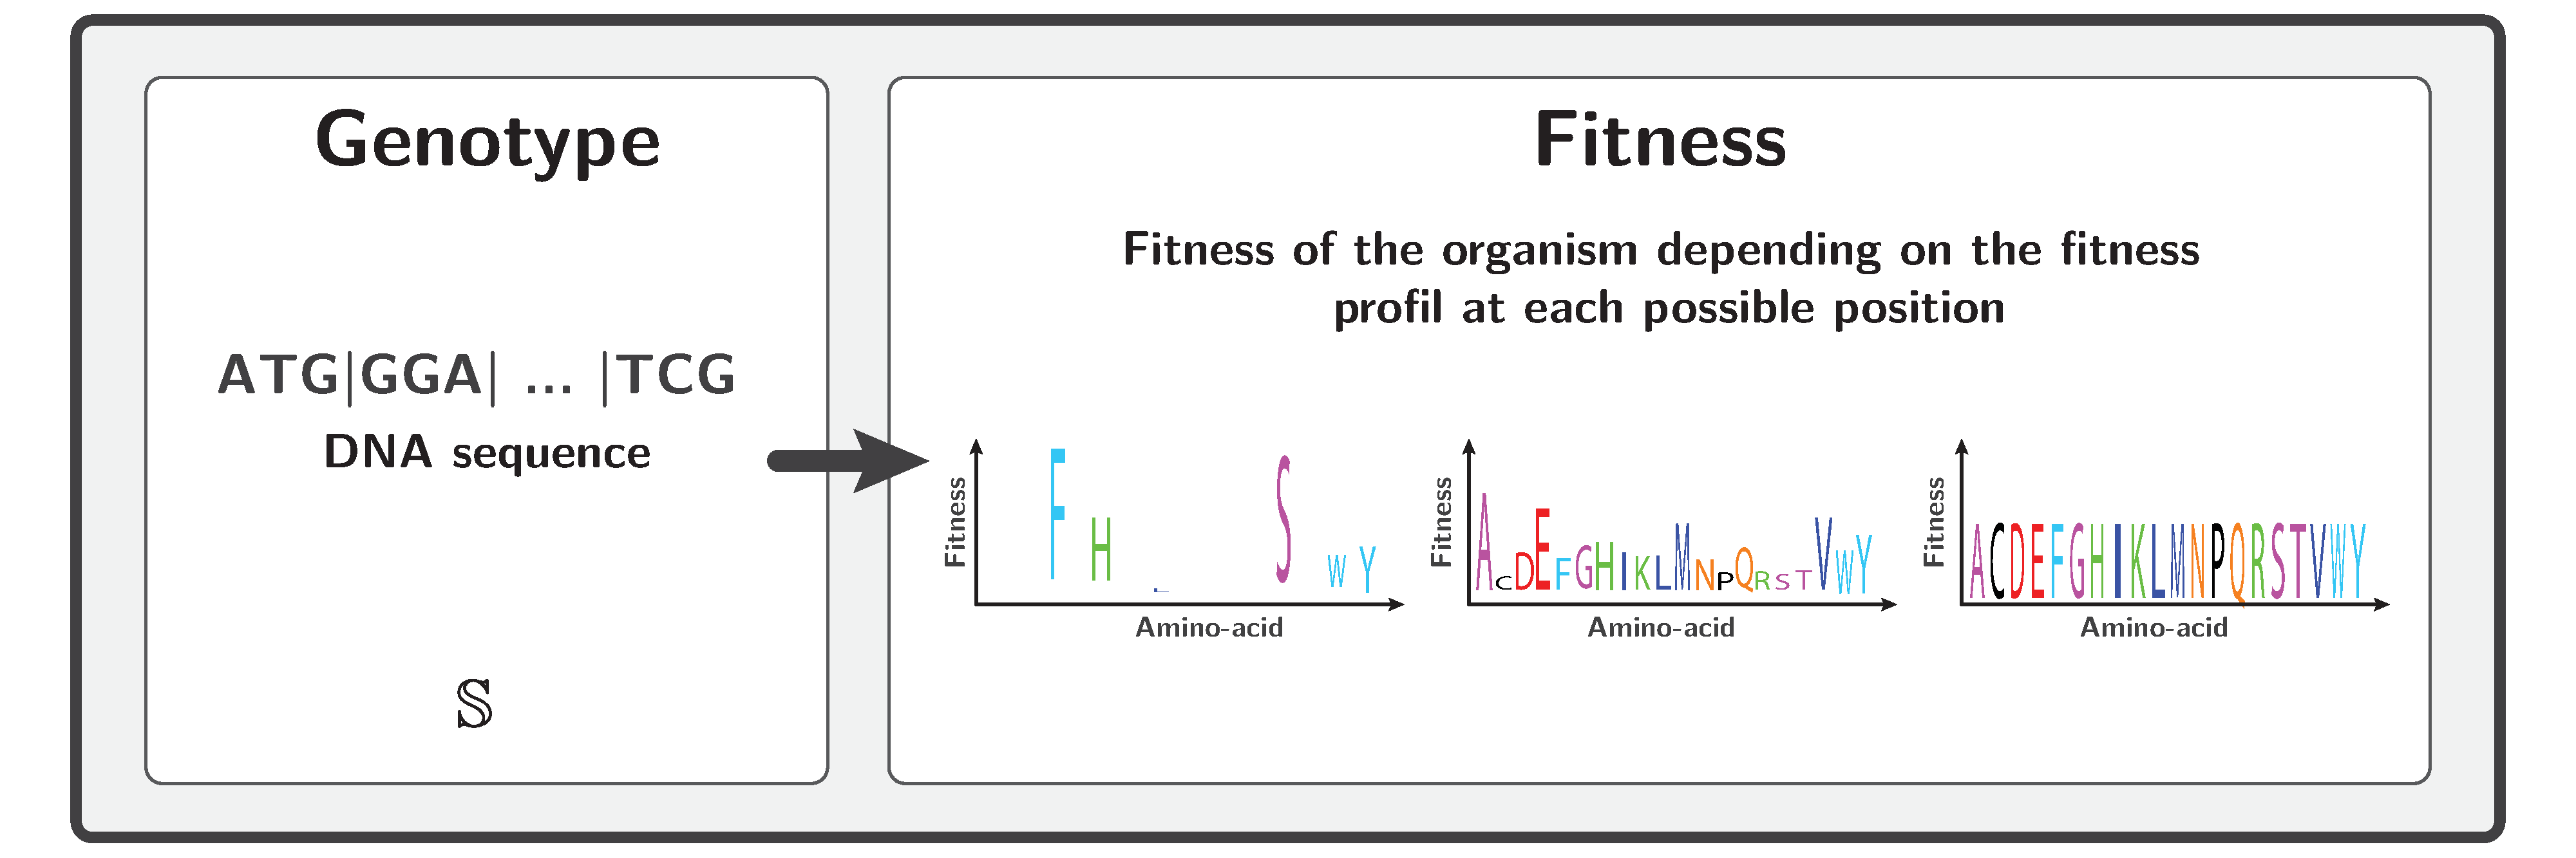
\includegraphics[width=\textwidth] {ModelSimuDiv}
\end{center}

The next change in the protein coding \acrshort{DNA} and the time to next the event is chosen using Gillespie algorithm, according to the rates of substitution between codons:
\begin{equation}
{\submatrix_{\itoj}}
    = \mu_{\itoj} \dfrac{4 \Ne s \left( \mathbb{S}^{t},\mathbb{S}^{t+1}\right)}{{1 - \e^{-4 \Ne s \left( \mathbb{S}^{t},\mathbb{S}^{t+1}\right)} }},
\end{equation}
where ${\submatrix_{\itoj}} = \mu_{\itoj}$ in the case of synonymous substitutions.


\begin{figure}[H]
    \centering
    \begin{minipage}{0.32\linewidth}
        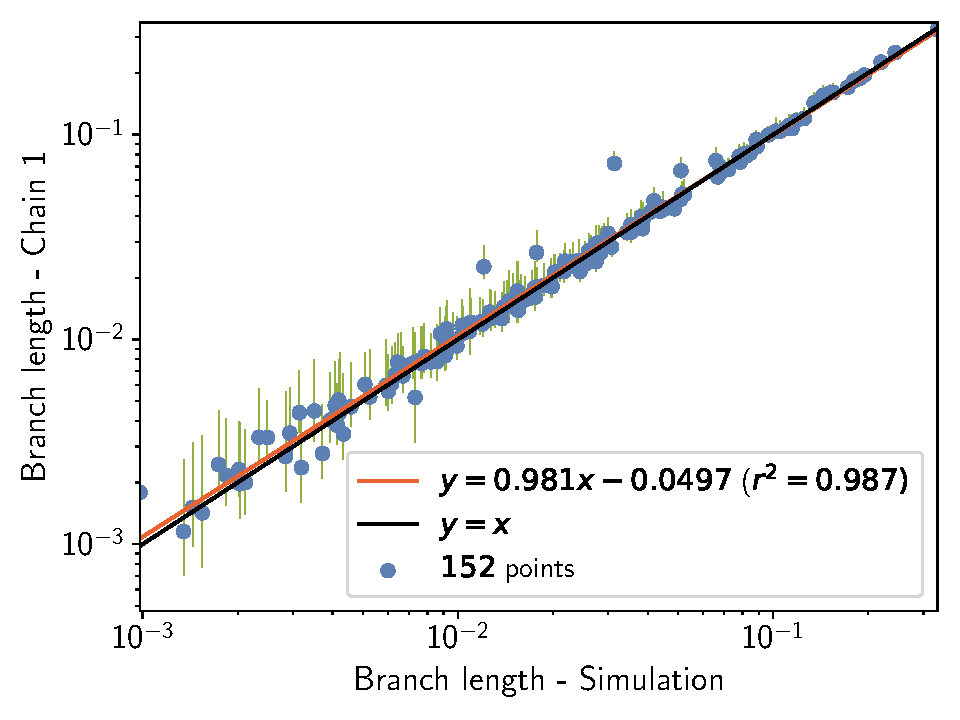
\includegraphics[width=\linewidth, page=1]{simulations/BranchWise_SimuDiv_SiteMutSelBranchNe_BranchCorrelation_Log10BranchLength}
    \end{minipage} \hfill
    \begin{minipage}{0.32\linewidth}
        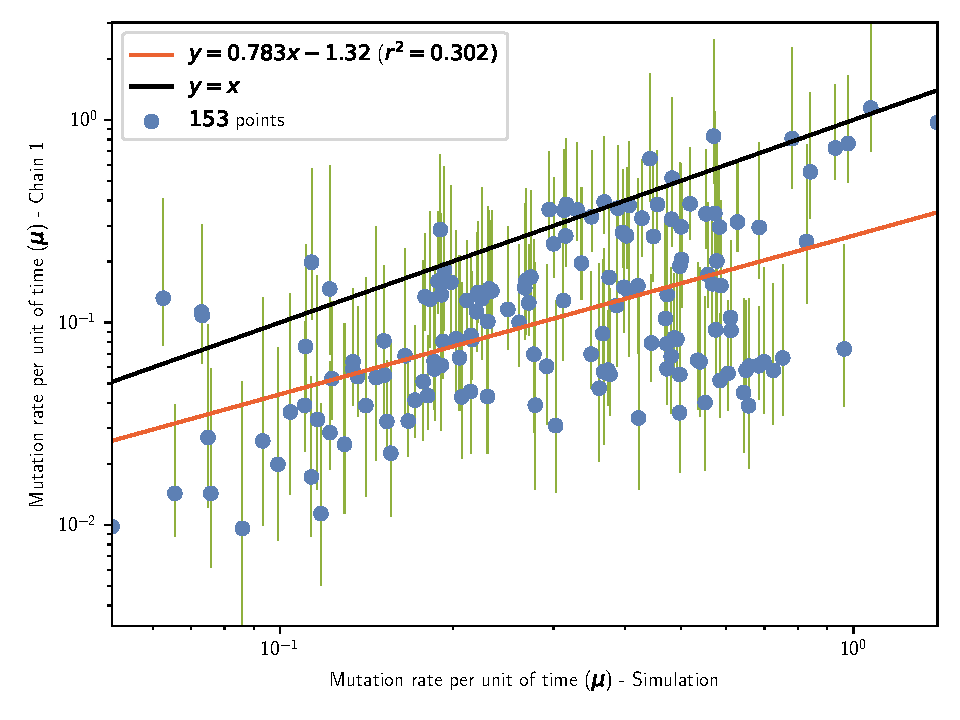
\includegraphics[width=\linewidth, page=1]{simulations/BranchWise_SimuDiv_SiteMutSelBranchNe_BranchCorrelation_LogMutationRatePerTime}
    \end{minipage} \hfill
    \begin{minipage}{0.32\linewidth}
        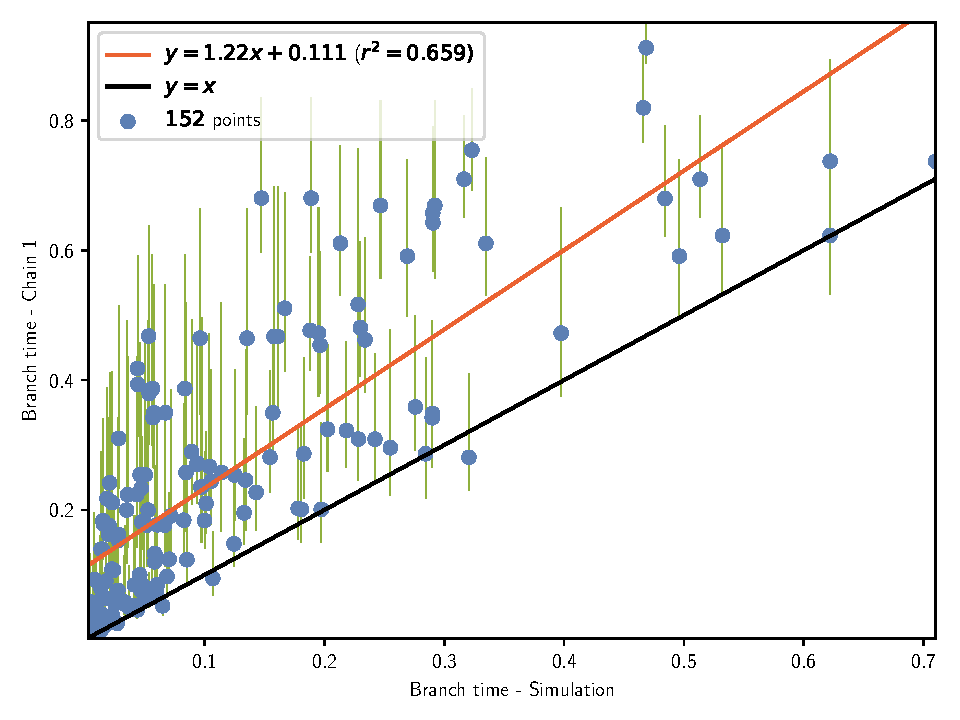
\includegraphics[width=\linewidth, page=1]{simulations/BranchWise_SimuDiv_SiteMutSelBranchNe_BranchCorrelation_BranchTime}
    \end{minipage} \hfill
    \begin{minipage}{0.32\linewidth}
        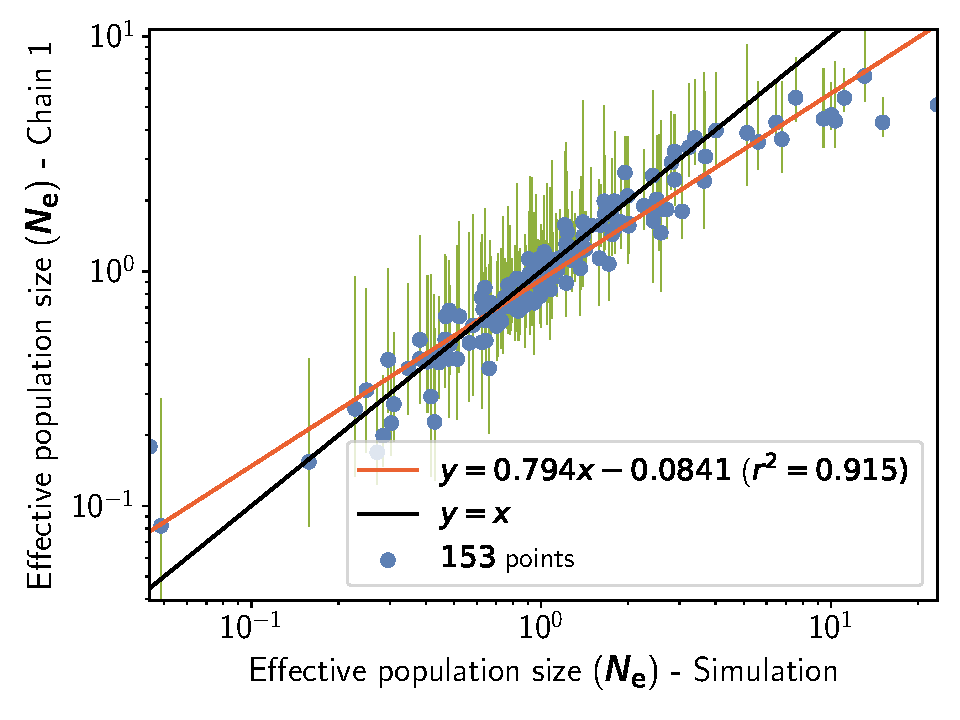
\includegraphics[width=\linewidth, page=1]{simulations/BranchWise_SimuDiv_SiteMutSelBranchNe_BranchCorrelation_LogPopulationSize}
    \end{minipage}
    \begin{minipage}{0.32\linewidth}
        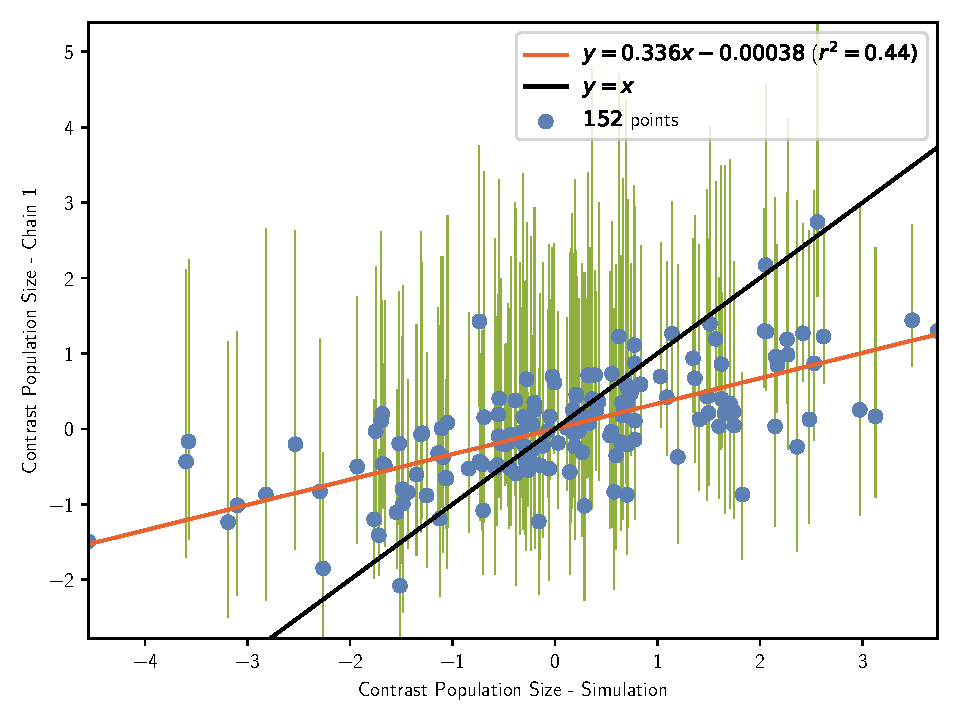
\includegraphics[width=\linewidth, page=1]{simulations/BranchWise_SimuDiv_SiteMutSelBranchNe_BranchCorrelation_ContrastPopulationSize}
    \end{minipage} \hfill
    \caption[Inferred branch parameters for SimuDiv]{
    Inferred branch parameters under simulation accounting for long term fluctuation of $\Ne$, mutation rate per generation and generation time.
    }
\end{figure}


\begin{figure}[H]
    \centering
    \begin{minipage}{0.49\linewidth}
        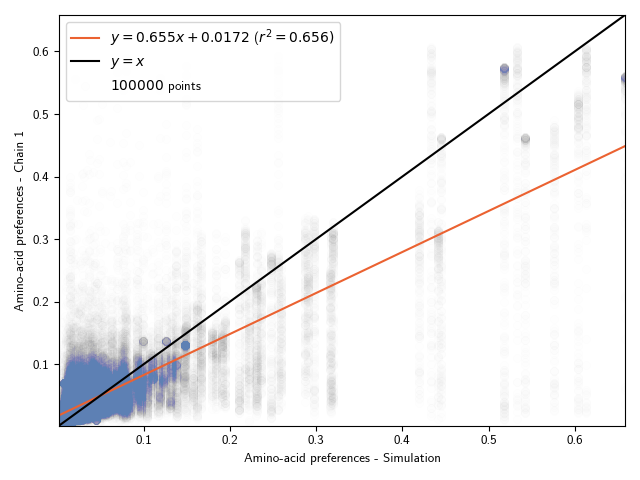
\includegraphics[width=\linewidth, page=1]{simulations/BranchWise_SimuDiv_SiteMutSelBranchNe_ProfileCorrelation.png}
    \end{minipage} \hfill
    \begin{minipage}{0.49\linewidth}
        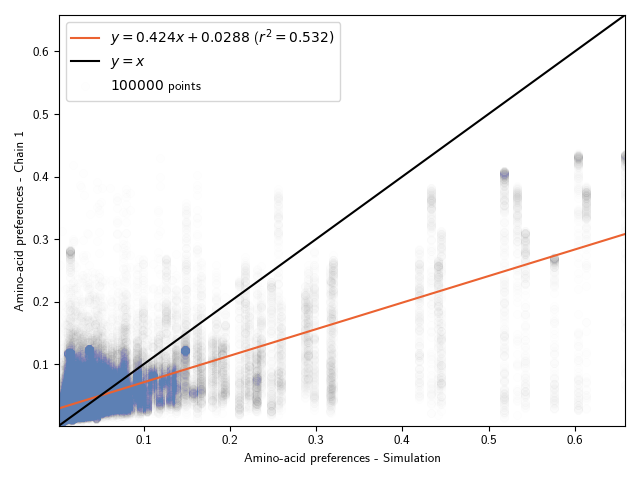
\includegraphics[width=\linewidth, page=1]{simulations/BranchWise_SimuDiv_SiteMutSel_ProfileCorrelation.png}
    \end{minipage}
    \caption[Inferred site amino-acid profiles for SimuDiv]{
    Inferred and simulated site specific amino-acid profiles under simulation accounting for long term fluctuation of $\Ne$, mutation rate per generation and generation time.
    Estimation with fluctuating branch $\Ne$ (left panel) or constant $\Ne$ (right panel).}
\end{figure}

\begin{table}[H]
    \centering
    \noindent\adjustbox{max width=\textwidth}{%
    \begin{tabu}{|c|c|c|}
        \hline
        \textbf{Experiment} & $\langle \entropy \rangle$ (\textbf{branch} $\Ne$) & $\langle \entropy \rangle$ (\textbf{constant} $\Ne$) \\ \hline
        \hline
        SimuDiv, chain~1 & $2.30 \pm 0.04$ & $2.45 \pm 0.02$\\ \hline
        SimuDiv, chain 2 & $2.30 \pm 0.04$ & $2.45 \pm 0.02$\\ \hline
    \end{tabu}}
    \caption[Inferred amino-acids entropy for SimuDiv]{
    Estimated amino-acids entropy.
    Simulation accounting for long term fluctuation of $\Ne$, mutation rate per generation and generation time.
    Estimated with the inference model of site selection for amino acid, and branch fluctuation of $\Ne$ (left column), or under the assumption of constant $\Ne$ (right column)}
\end{table}

\subsection{Wright-Fisher with polymorphism}

The evolutionary dynamics was formalized as a Wright-Fisher model with mutation, selection and drift
The population is assumed to be panmictic, with effective population size $\Ne$ and with non-overlapping generations.

\begin{center}
    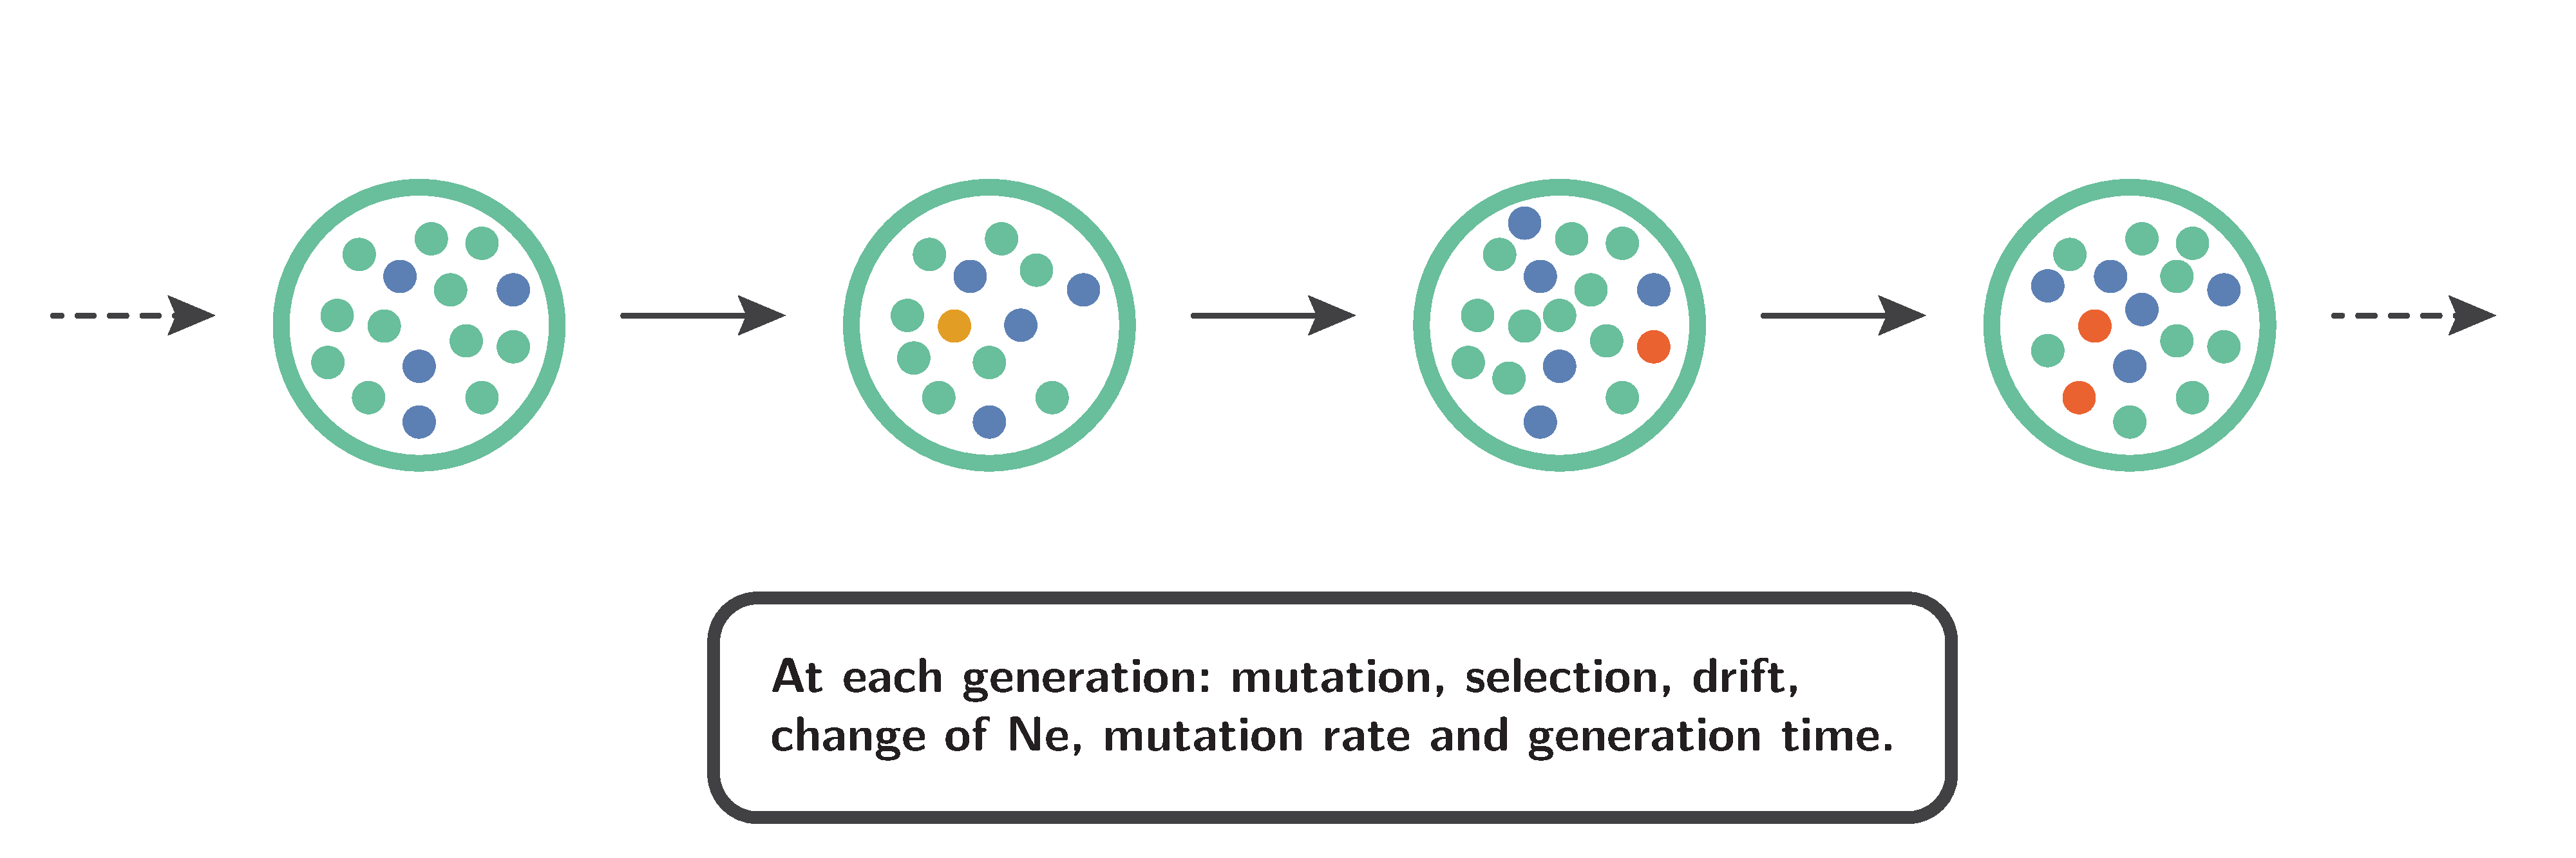
\includegraphics[width=\textwidth] {ModelSimuPoly}
\end{center}

\begin{figure}[H]
    \centering
    \begin{minipage}{0.32\linewidth}
        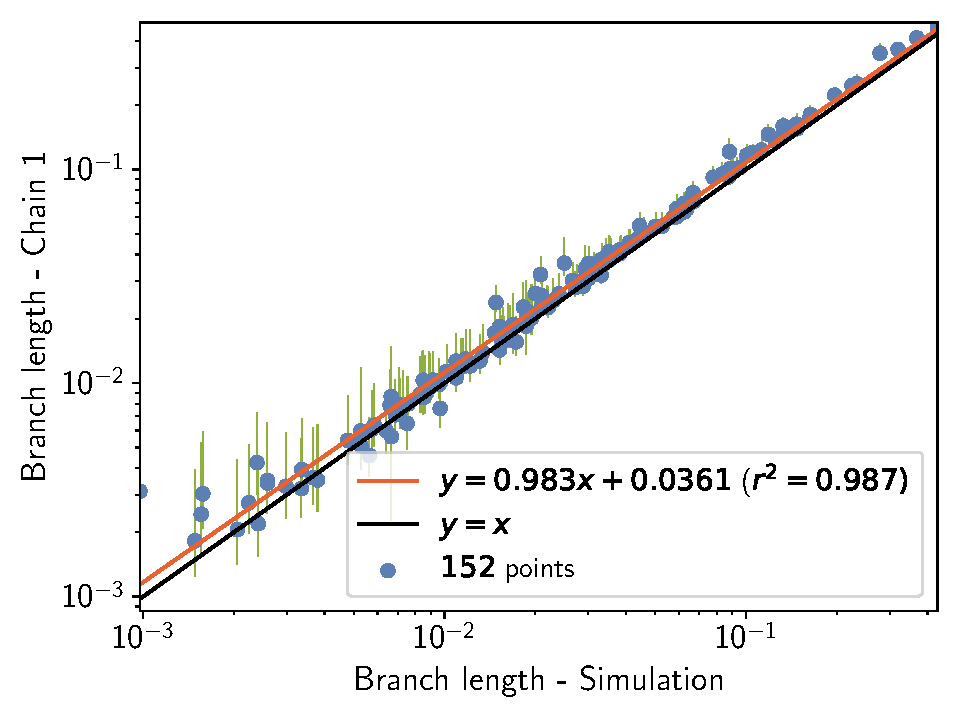
\includegraphics[width=\linewidth, page=1]{simulations/SimuPoly_SiteMutSelBranchNe_BranchCorrelation_Log10BranchLength}
    \end{minipage} \hfill
    \begin{minipage}{0.32\linewidth}
        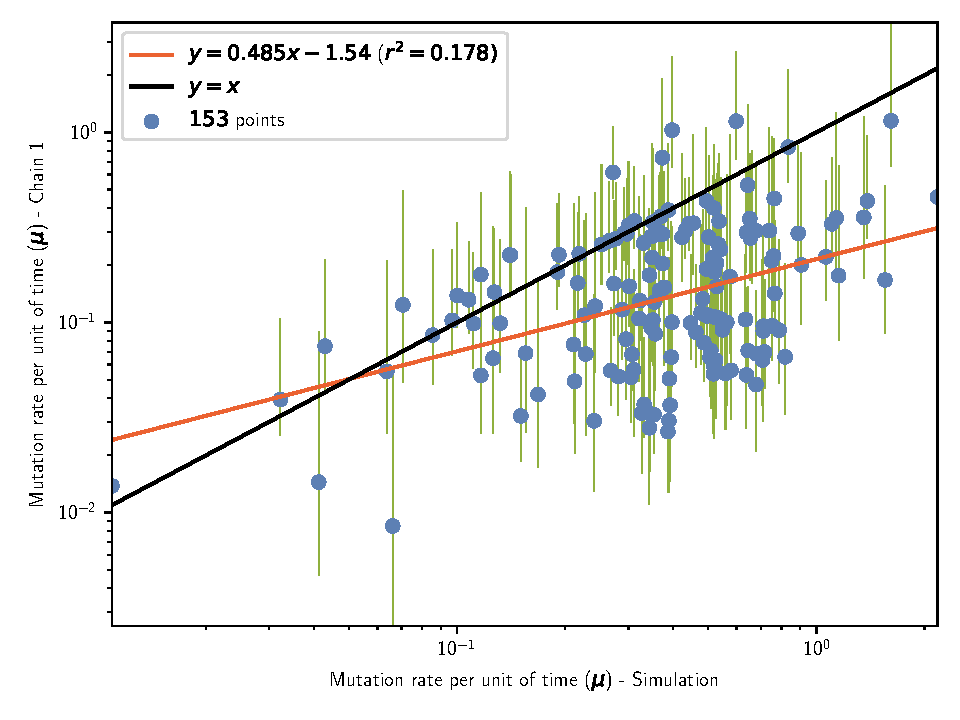
\includegraphics[width=\linewidth, page=1]{simulations/SimuPoly_SiteMutSelBranchNe_BranchCorrelation_LogMutationRatePerTime}
    \end{minipage} \hfill
    \begin{minipage}{0.32\linewidth}
        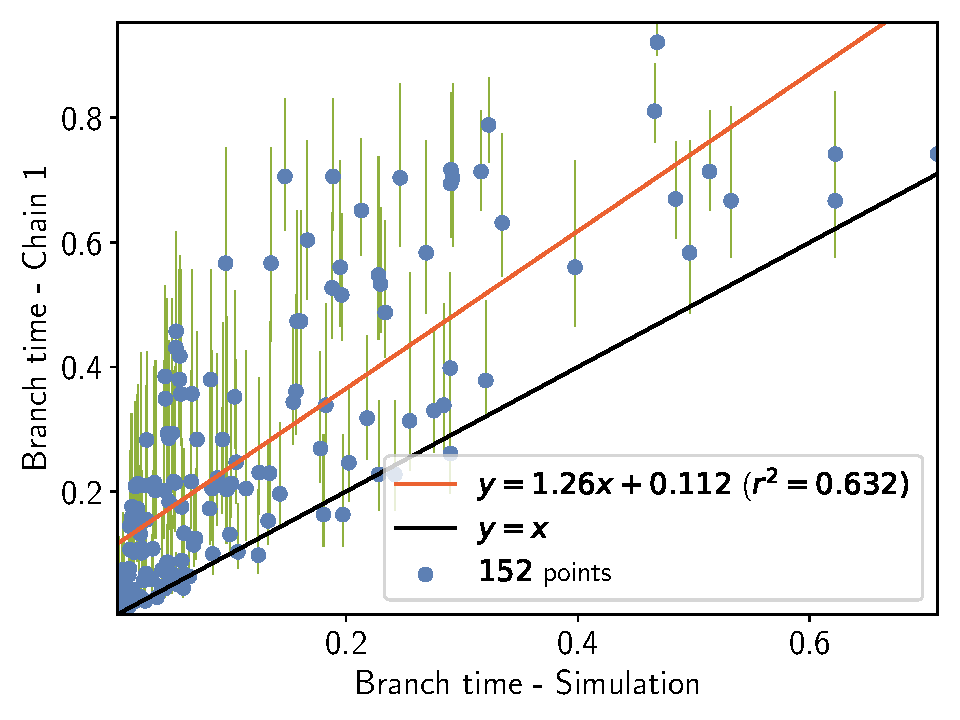
\includegraphics[width=\linewidth, page=1]{simulations/SimuPoly_SiteMutSelBranchNe_BranchCorrelation_BranchTime}
    \end{minipage} \hfill
    \begin{minipage}{0.32\linewidth}
        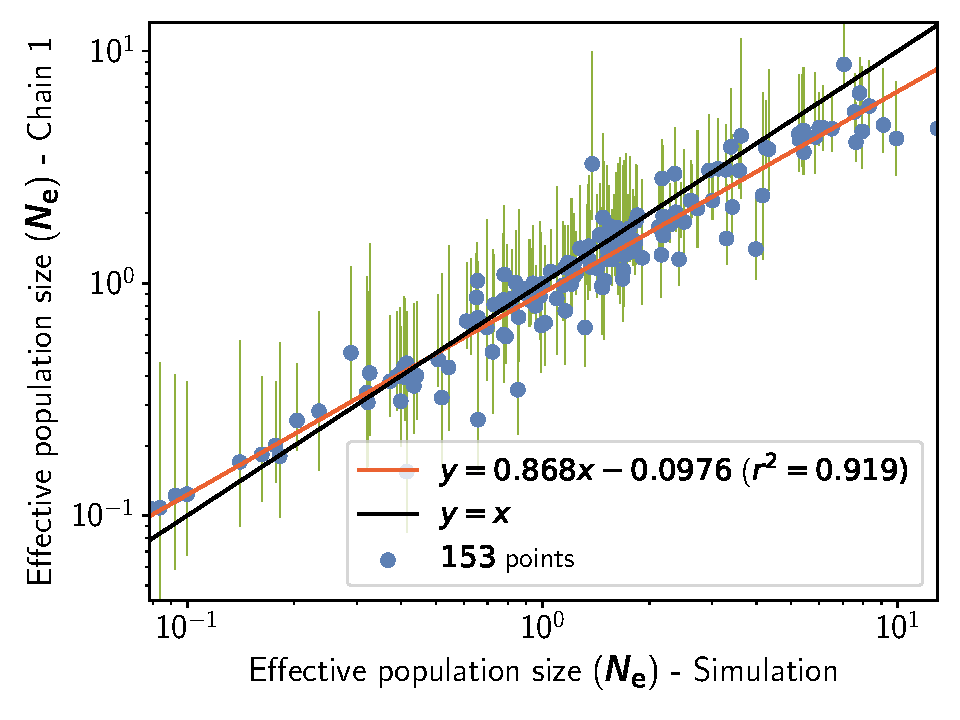
\includegraphics[width=\linewidth, page=1]{simulations/SimuPoly_SiteMutSelBranchNe_BranchCorrelation_LogPopulationSize}
    \end{minipage}
    \begin{minipage}{0.32\linewidth}
        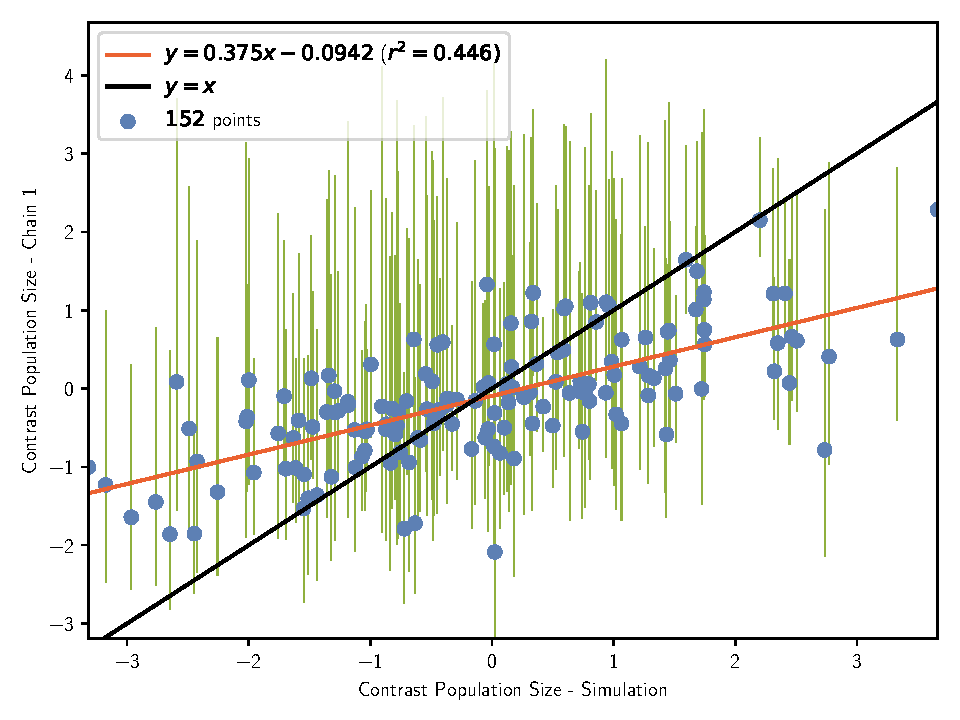
\includegraphics[width=\linewidth, page=1]{simulations/SimuPoly_SiteMutSelBranchNe_BranchCorrelation_ContrastPopulationSize}
    \end{minipage} \hfill
    \caption[Inferred branch parameters for SimuPoly]{
    Inferred branch parameters under simulation accounting for finite population effects, site linkage and short term fluctuation of $\Ne$.
    }
\end{figure}


\begin{figure}[H]
    \centering
    \begin{minipage}{0.49\linewidth}
        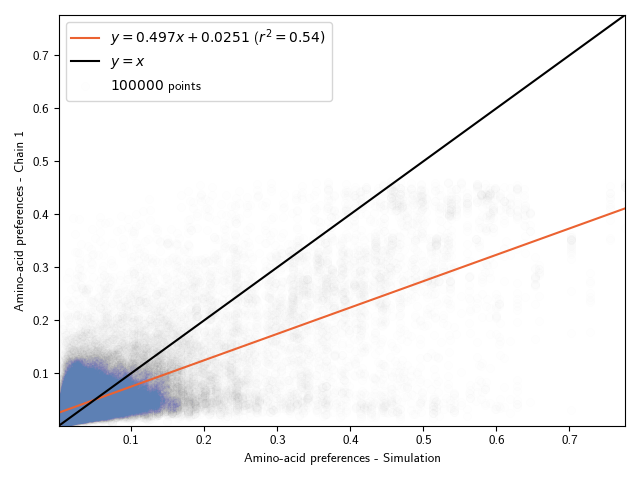
\includegraphics[width=\linewidth, page=1]{simulations/SimuPoly_SiteMutSelBranchNe_ProfileCorrelation.png}
    \end{minipage} \hfill
    \begin{minipage}{0.49\linewidth}
        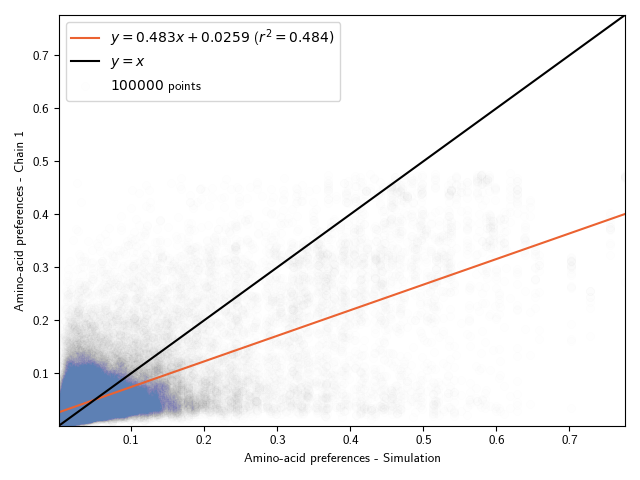
\includegraphics[width=\linewidth, page=1]{simulations/SimuPoly_SiteMutSel_ProfileCorrelation.png}
    \end{minipage}
    \caption[Inferred site amino-acid profiles for SimuPoly]{
    Inferred and simulated site specific amino-acid profiles under simulation accounting for finite population effects, site linkage and short term fluctuation of $\Ne$.
    Estimation with fluctuating branch $\Ne$ (left panel) or constant $\Ne$ (right panel).}
\end{figure}

\begin{table}[H]
    \centering
    \noindent\adjustbox{max width=\textwidth}{%
    \begin{tabu}{|c|c|c|}
        \hline
        \textbf{Experiment} & $\langle \entropy \rangle$ (\textbf{branch} $\Ne$) & $\langle \entropy \rangle$ (\textbf{constant} $\Ne$) \\ \hline
        \hline
        SimuPoly, chain~1 & $2.47 \pm 0.03$ & $2.37 \pm 0.02$\\ \hline
        SimuPoly, chain 2 & $2.47 \pm 0.03$ & $2.37 \pm 0.02$\\ \hline
    \end{tabu}}
    \caption[Inferred amino-acid entropy for SimuPoly]{
    Estimated amino-acids entropy under simulation accounting for finite population effects, site linkage and short term fluctuation of $\Ne$.
    Obtained with the inference model of site selection for amino acid, and branch fluctuation of $\Ne$ (left column), or under the assumption of constant $\Ne$ (right column)}
\end{table}

\subsection{Fisher geometric landscape}
\label{subsec:fisher-geometric-landscape}

We simulated substitutions in a protein using an adaptation of Fisher's geometric landscape.
In the original context, the phenotype is a vector ($\phenoGeo$) in a multidimensional space, where the number of dimensions is often termed complexity.
From a phenotype, the fitness is a monotonously decreasing function of the phenotype distance to $0$.
The exact functional phenotype-fitness map depends on $2$ external parameters controlling for strength ($\alpha$) and epistasis ($\beta$).
If the phenotype-fitness map is explicit, the genotype-phenotype map is more pervasive.
Mutations are seen has displacement of the phenotype in the multidimensional space.
Beneficial mutations are moving the phenotype closer to $0$, whereas deleterious mutations are moving the phenotype further away.
In such original context, the distribution of mutational effects is not dependent on the current genotype, but this can be relaxed using a genotype-phenotype map.\\

In a protein context, the genotype-phenotype map can be defined by assigning to each of the $20$ amino acid a vector in the multidimensional space.
Since different sites of the protein do not have the same physico-chimical properties, we can define a specific genotype-phenotype map for each position of the sequence.
Overall, the protein phenotype is computed as the sum of site-specific multidimensional vectors, obtained by accessing the amino acid present at each site of the protein.
From a \acrshort{DNA} sequence $\mathbb{S}^t$ after $t$ substitutions, the protein's phenotype is given by:
\begin{equation}
    \phenoGeo\left(\mathbb{S}^{t}\right) = \sum\limits_{1 \leq \site \leq \Nsite} \phenoGeo_{\site} \left(\mathbb{S}^t(\site) \right),
\end{equation}
where $\phenoGeo_{\site}$ is the genotype-phenotype map at site $\site$.\\

And the Wrightian fitness of $\mathbb{S}^t$ is :
\begin{equation}
    w\left( \phenoGeo\left(\mathbb{S}^{t}\right) \right) = e^{-\alpha \left| \phenoGeo\left(\mathbb{S}^{t}\right) \right|^{\beta}},
\end{equation}
where strength ($\alpha > 0$) and epistasis ($\beta$) are parameters of the fitness function.
\begin{center}
    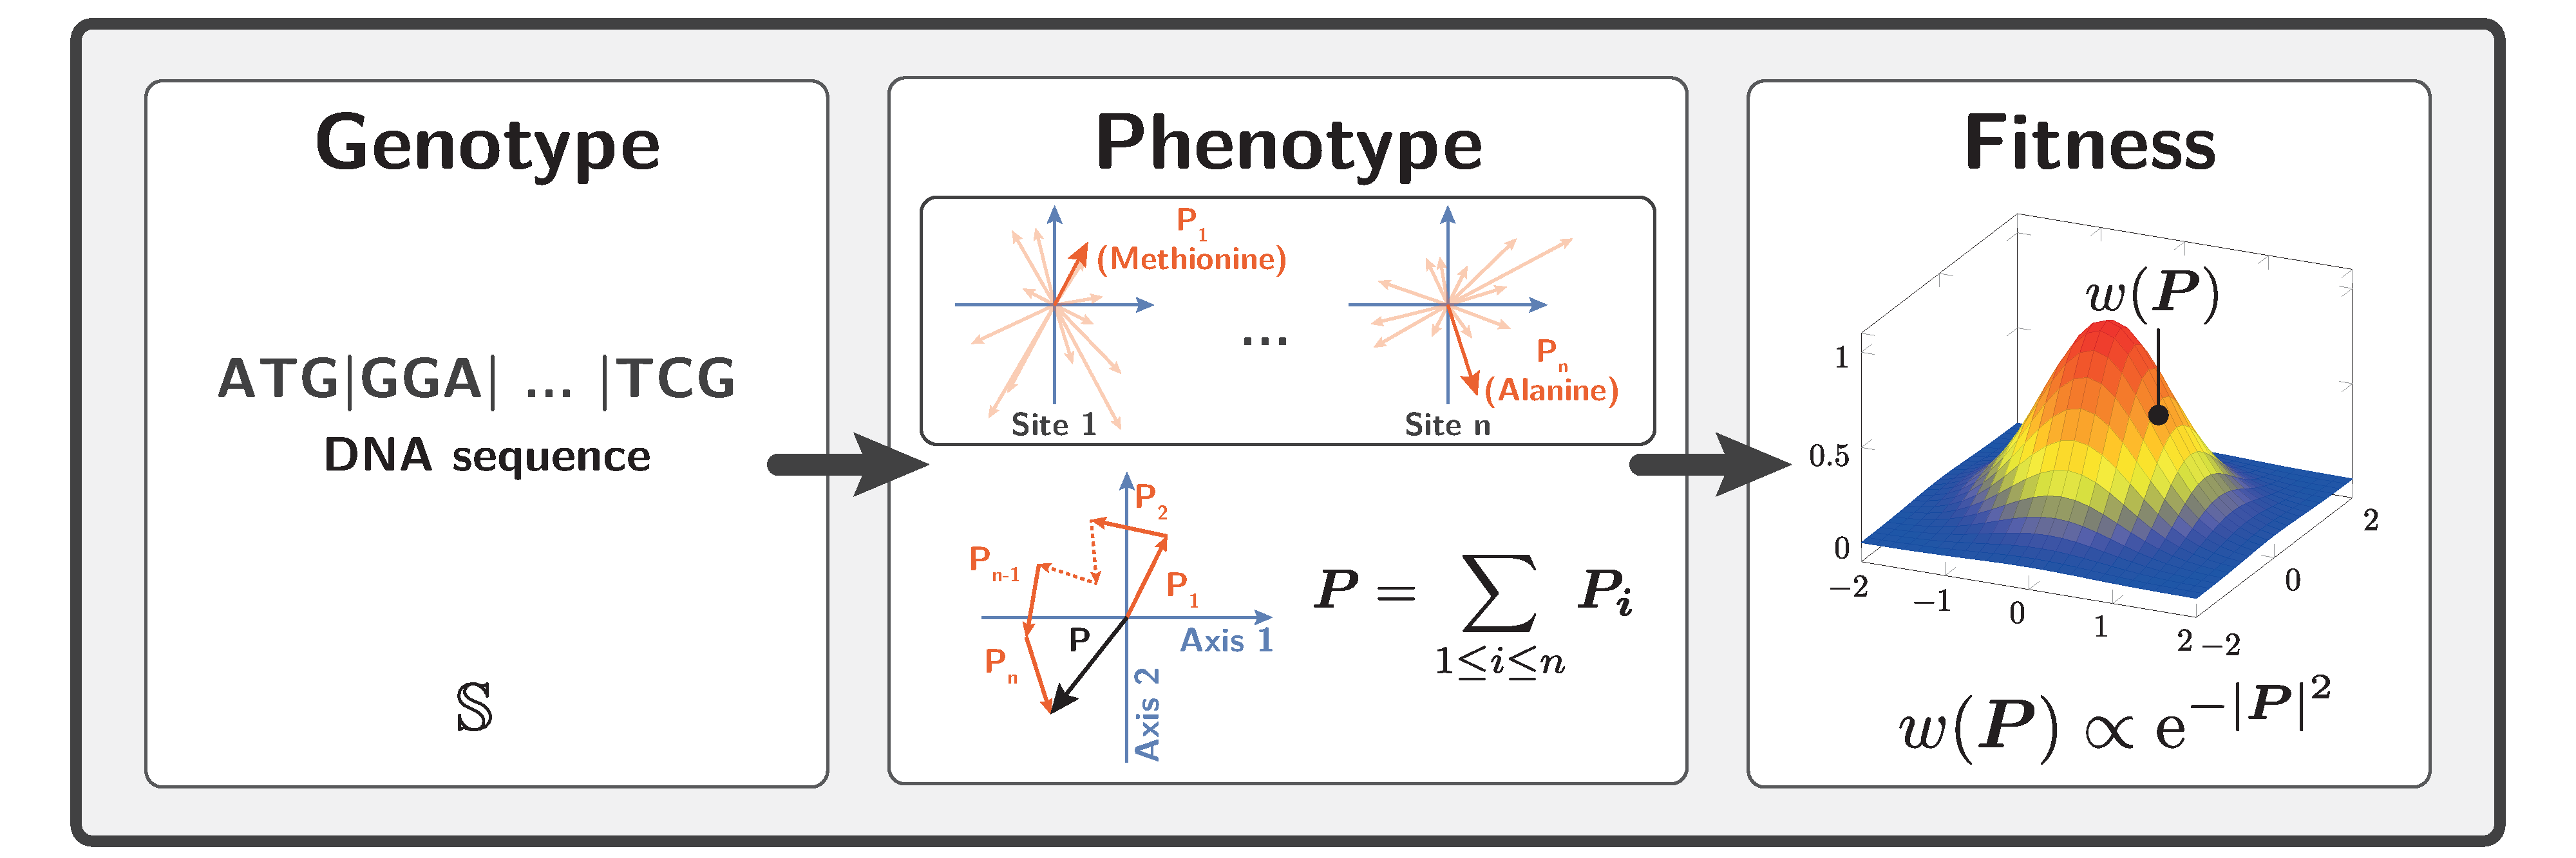
\includegraphics[width=\textwidth] {ModelSimuGeo}
\end{center}
For each possible mutant ($t+1$ substitutions), we compute $\phenoGeo\left(\mathbb{S}^{t+1}\right)$ from the updated sequence $\mathbb{S}^{t+1}$, and subsequently the selection coefficient of the mutant:
\begin{equation}
    s \left( \mathbb{S}^{t},\mathbb{S}^{t+1}\right) = \dfrac{ w\left( \phenoGeo\left(\mathbb{S}^{t+1}\right) \right) - w\left( \phenoGeo\left(\mathbb{S}^{t}\right) \right)}{w\left( \phenoGeo\left(\mathbb{S}^{t}\right) \right)}.
\end{equation}
The next change in the protein coding \acrshort{DNA} and the time to next the event is chosen using Gillespie algorithm, according to the rates of substitution between codons:
\begin{equation}
{\submatrix_{\itoj}}
    = \mu_{\itoj} \dfrac{4 \Ne s \left( \mathbb{S}^{t},\mathbb{S}^{t+1}\right)}{{1 - \e^{-4 \Ne s \left( \mathbb{S}^{t},\mathbb{S}^{t+1}\right)} }},
\end{equation}
where ${\submatrix_{\itoj}} = \mu_{\itoj}$ in the case of synonymous substitutions.

\begin{figure}[H]
    \centering
    \begin{minipage}{0.32\linewidth}
        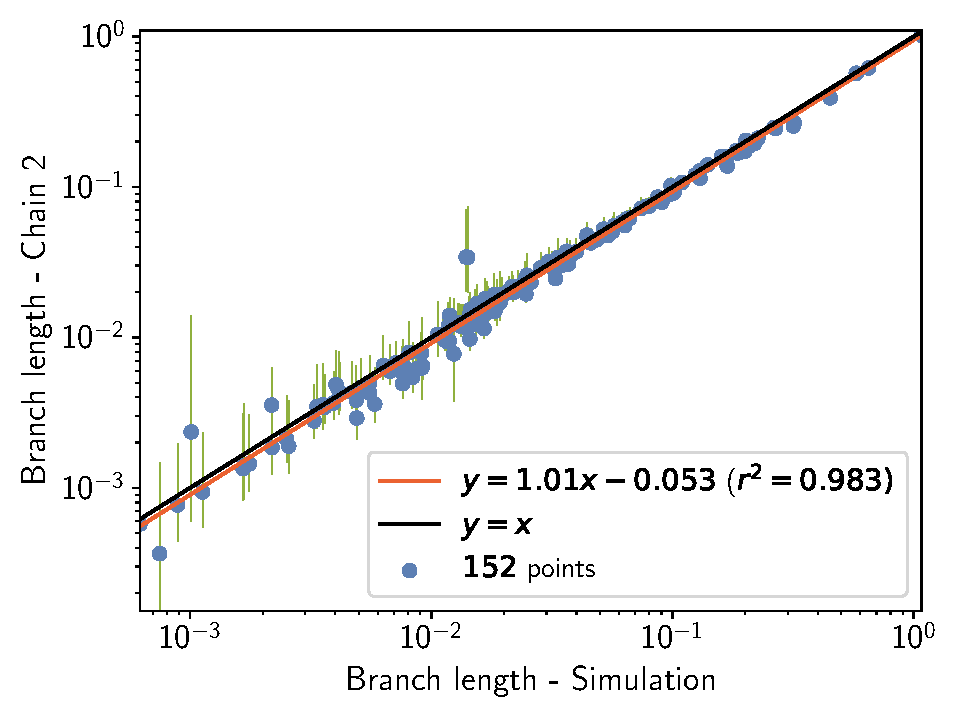
\includegraphics[width=\linewidth, page=1]{simulations/SimuGeo_SiteMutSelBranchNe_BranchCorrelation_Log10BranchLength}
    \end{minipage} \hfill
    \begin{minipage}{0.32\linewidth}
        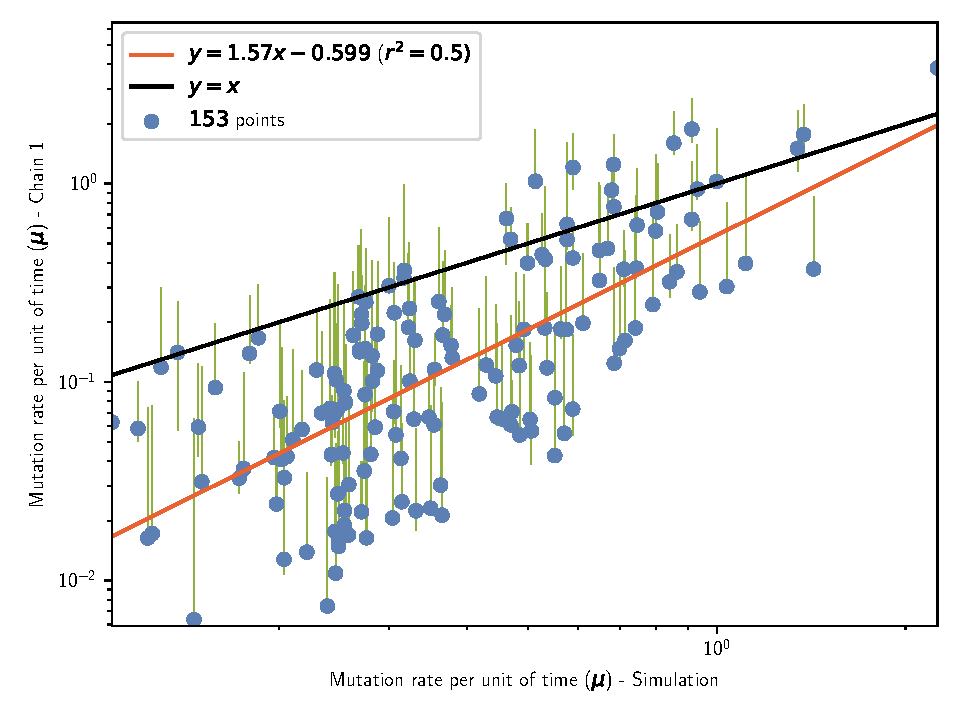
\includegraphics[width=\linewidth, page=1]{simulations/SimuGeo_SiteMutSelBranchNe_BranchCorrelation_LogMutationRatePerTime}
    \end{minipage} \hfill
    \begin{minipage}{0.32\linewidth}
        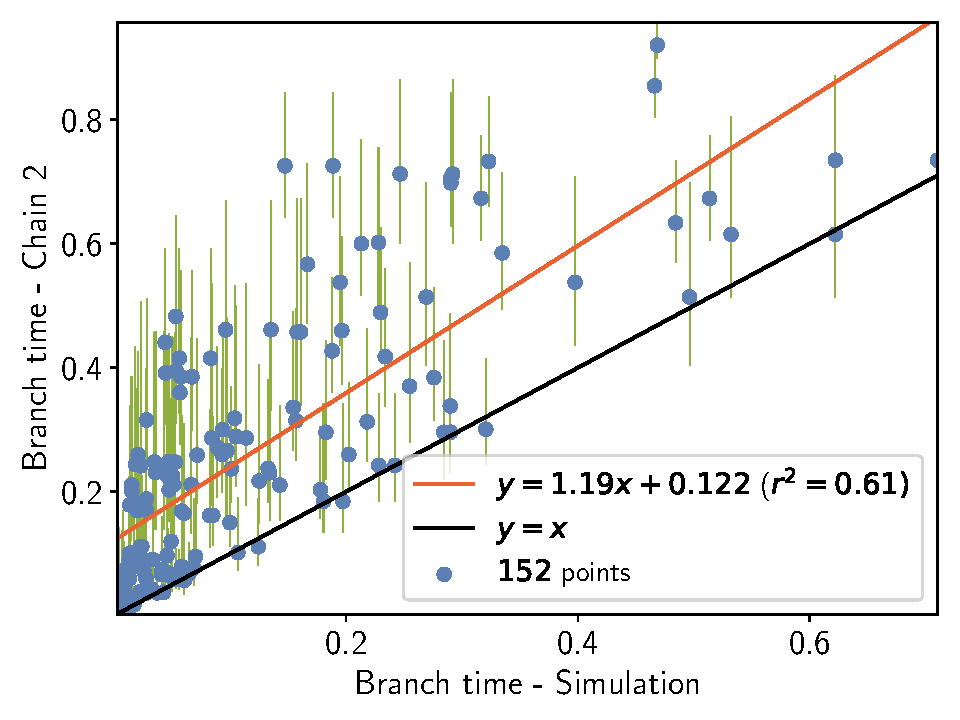
\includegraphics[width=\linewidth, page=1]{simulations/SimuGeo_SiteMutSelBranchNe_BranchCorrelation_BranchTime}
    \end{minipage} \hfill
    \begin{minipage}{0.32\linewidth}
        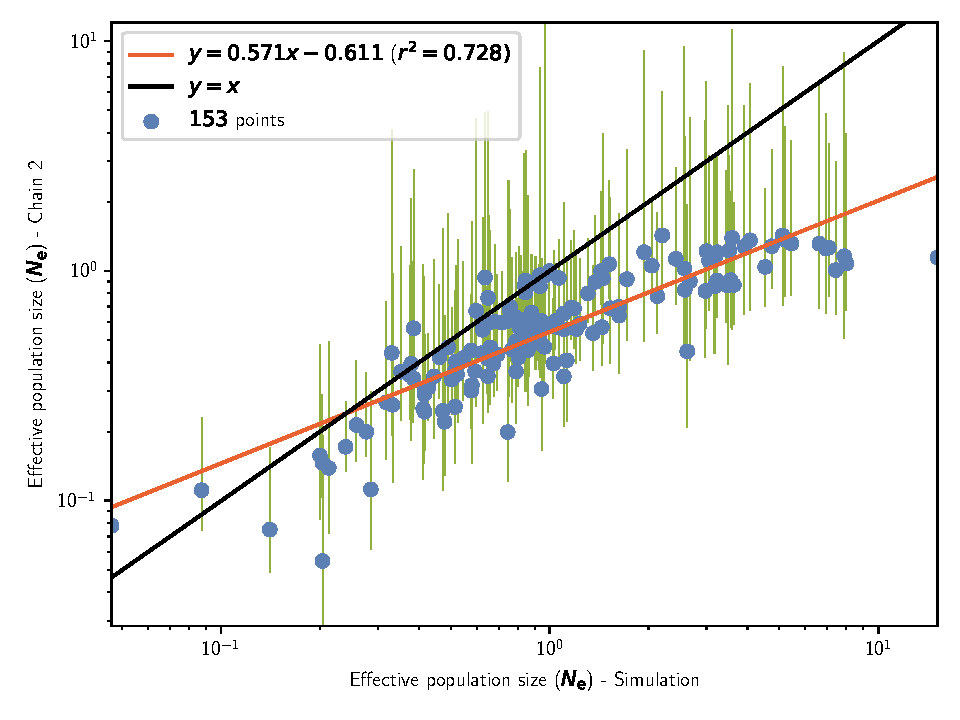
\includegraphics[width=\linewidth, page=1]{simulations/SimuGeo_SiteMutSelBranchNe_BranchCorrelation_LogPopulationSize}
    \end{minipage}
    \begin{minipage}{0.32\linewidth}
        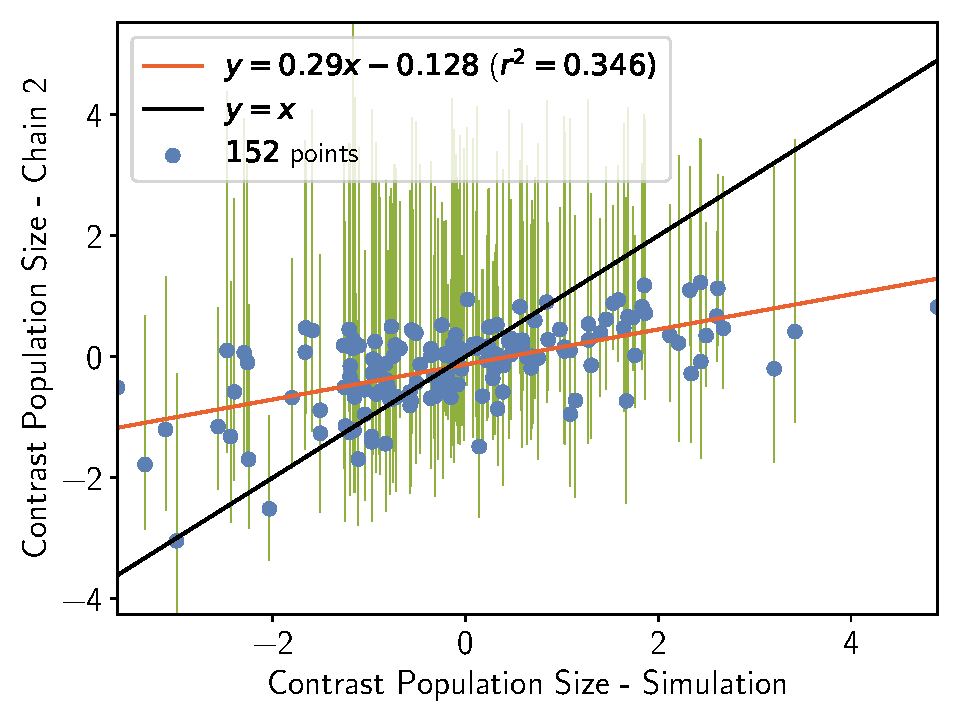
\includegraphics[width=\linewidth, page=1]{simulations/SimuGeo_SiteMutSelBranchNe_BranchCorrelation_ContrastPopulationSize}
    \end{minipage} \hfill
    \caption[Inferred branch parameters for SimuGeo]{
    Inferred branch parameters under simulation accounting for site epistasis in geometric landscape, thus fluctuation of the selection coefficient along the phylogeny.
    }
\end{figure}


\begin{table}[H]
    \centering
    \noindent\adjustbox{max width=\textwidth}{%
    \begin{tabu}{|c|c|c|}
        \hline
        \textbf{Experiment} & $\langle \entropy \rangle$ (\textbf{branch} $\Ne$) & $\langle \entropy \rangle$ (\textbf{constant} $\Ne$) \\ \hline
        \hline
        SimuGeo, chain~1 & $2.27 \pm 0.02$ & $2.46 \pm 0.02$\\ \hline
        SimuGeo, chain 2 & $2.23 \pm 0.04$ & $2.46 \pm 0.02$\\ \hline
    \end{tabu}}
    \caption[Amino-acid entropy for SimuGeo]{
    Estimated amino-acid entropy under simulation accounting for site epistasis (geometric landscape), thus fluctuation of the selection coefficient along the phylogeny.
    Obtained with the inference model of site selection for amino acid, and branch fluctuation of $\Ne$ (left column), or under the assumption of constant $\Ne$ (right column)}
\end{table}

\subsection{Protein folding probability}
\label{subsec:protein-folding-probability}

We simulated substitutions in the protein phosphatase ($\Nsite=300$ codon sites) as in Goldstein \& Pollock (2017).
From a \acrshort{DNA} sequence $\mathbb{S}^t$ after $t$ substitutions, we compute the free energy of the folded state $\Base_{\mathrm{F}}\left(\mathbb{S}^{t}\right)$, using the $3$-dimensional structure of the folded state and pair-wise contact energies between neighboring amino-acid residues:
\begin{equation}
    G_{\mathrm{F}}\left(\mathbb{S}^{t}\right) = \sum\limits_{1 \leq \site \leq \Nsite} \sum\limits_{r \in \mathcal{N}(\site)} I \left(\mathbb{S}^t(\site), \mathbb{S}^t(r) \right),
\end{equation}
where $I(a,b)$ is the pair-wise contact energies between amino acid $a$ and $b$, using contact potentials estimated by Miya-zawa and Jernigan, and $\mathcal{N}(\site)$ are the neighbor residues of site $\site$ (closer than $7\angstrom$) in the $3$D structure.\\

The free energy of unfolded states $G_{\mathrm{U}}\left(\mathbb{S}^{t}\right)$ is approximated using $55$ decoy $3$D structures that supposedly represent a sample of possible unfolded states:
\begin{equation}
    G_{\mathrm{U}}\left(\mathbb{S}^{t}\right) = \langle G\left(\mathbb{S}^{t}\right) \rangle - kT \ln (1.0\mathrm{E}^{160}) - \dfrac{2 \left[ \langle G\left(\mathbb{S}^{t}\right)^2 \rangle - \langle G\left(\mathbb{S}^{t}\right) \rangle^2\right] }{kT}
\end{equation}
where the average $\langle . \rangle$ runs other the $55$ decoy $3$D structures, and $k$ is the Boltzmann constant and $T$ the temperature in Kelvin.\\

From the energy of folded and unfolded states, we can compute the difference in free energy between the states:
\begin{equation}
    \phenoFold\left(\mathbb{S}^{t}\right) = G_{\mathrm{F}}\left(\mathbb{S}^{t}\right) - G_{\mathrm{U}}\left(\mathbb{S}^{t}\right)
\end{equation}

Wrightian fitness is defined as the probability of our protein to be in the folded state:
\begin{equation}
    w(\phenoFold\left(\mathbb{S}^{t}\right)) = \dfrac{P_{\mathrm{F}}\left(\mathbb{S}^{t}\right)}{P_{\mathrm{F}}\left(\mathbb{S}^{t}\right) + P_{\mathrm{U}}\left(\mathbb{S}^{t}\right)} = \dfrac{e^{-\beta G_{\mathrm{F}}\left(\mathbb{S}^{t}\right) }}{e^{-\beta G_{\mathrm{F}} \left(\mathbb{S}^{t}\right) } + e^{-\beta G_{\mathrm{U}}\left(\mathbb{S}^{t}\right) }} = \dfrac{1}{1 + e^{\beta \phenoFold\left(\mathbb{S}^{t}\right) }},
\end{equation}
where $\beta$ is the inverse of the temperature ($\beta=1/kT$).
\begin{center}
    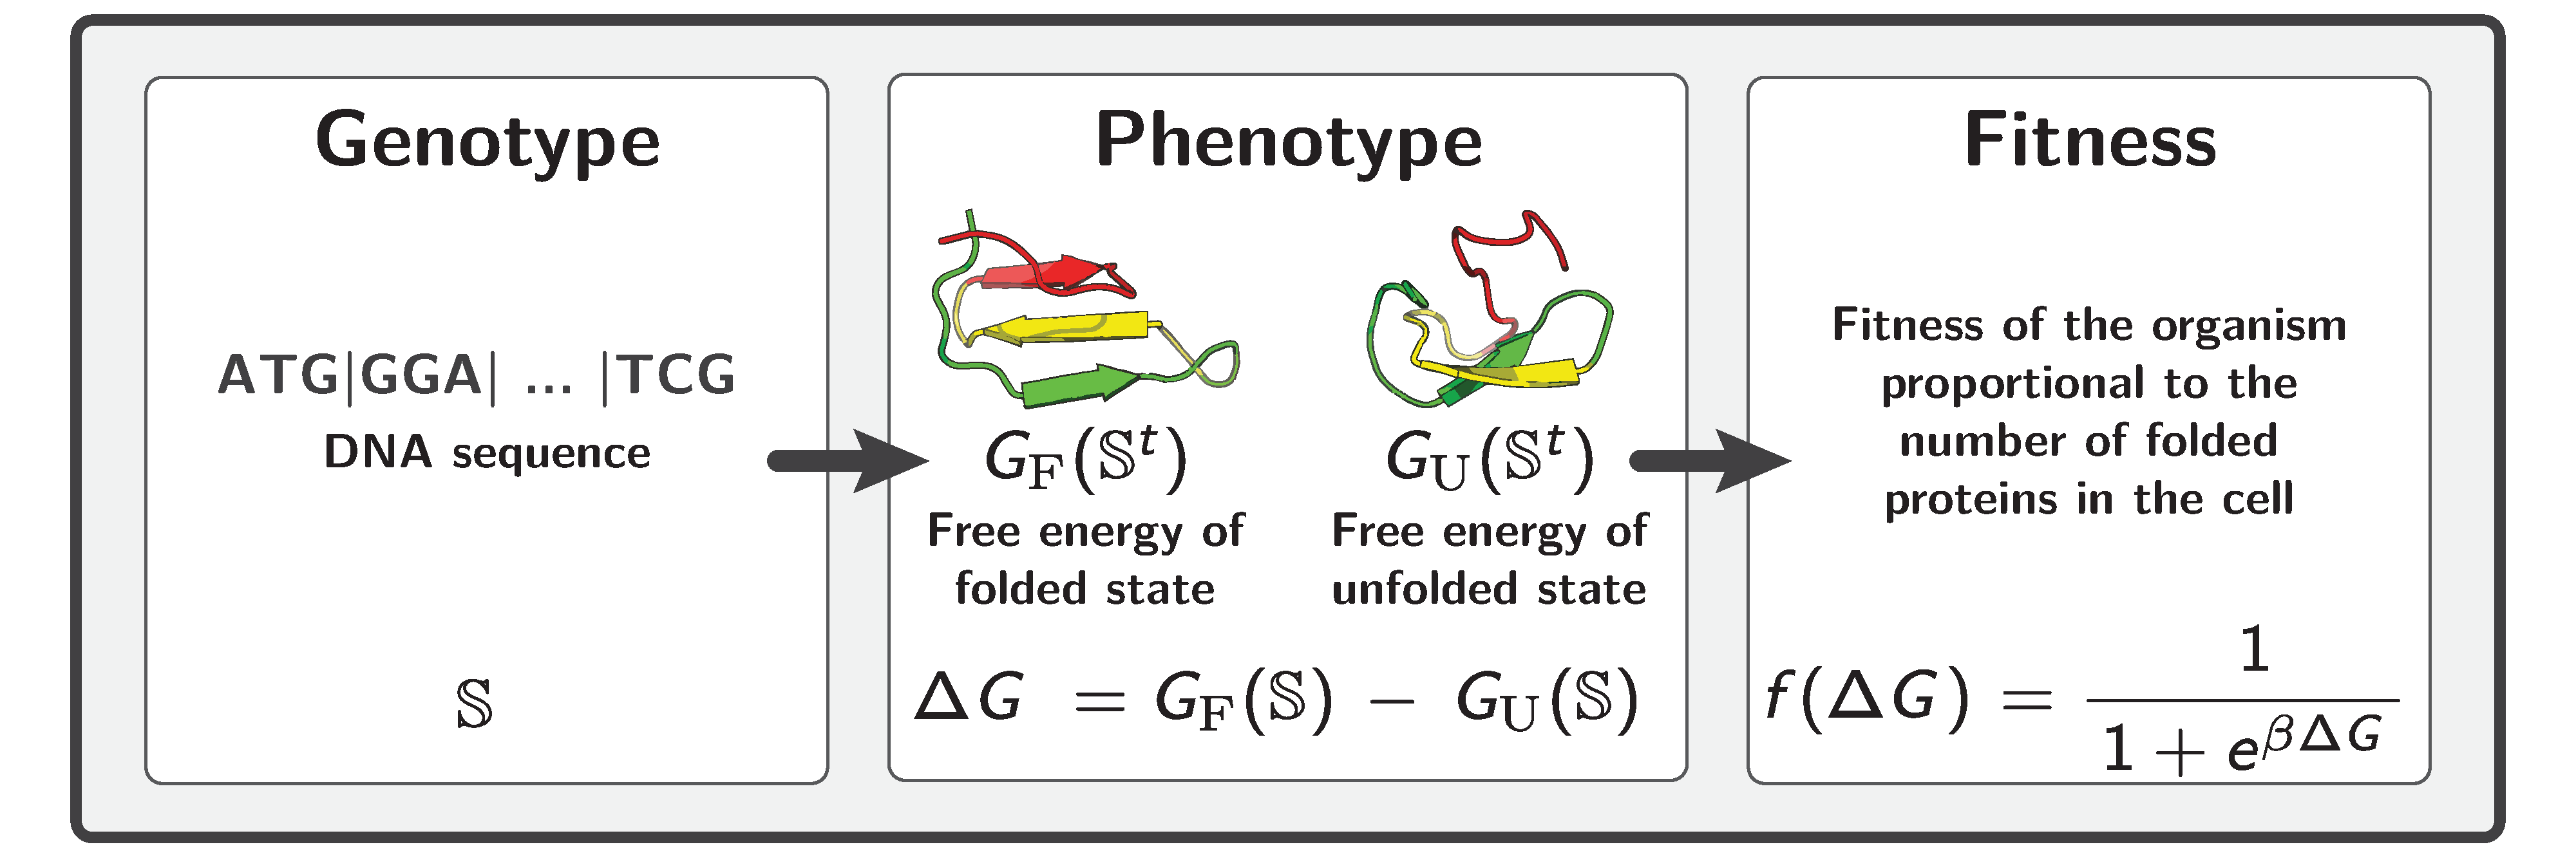
\includegraphics[width=\textwidth] {ModelSimuFold}
\end{center}
For each possible mutant ($t+1$ substitutions), we compute $\phenoFold^{t+1}$ from the updated sequence $\mathbb{S}^{t+1}$, and subsequently the selection coefficient of the mutant:
\begin{equation}
    s \left( \mathbb{S}^{t},\mathbb{S}^{t+1}\right) = \dfrac{ w\left( \phenoFold\left(\mathbb{S}^{t+1}\right) \right) - w\left( \phenoFold\left(\mathbb{S}^{t}\right) \right)}{w\left( \phenoFold\left(\mathbb{S}^{t}\right) \right)}.
\end{equation}
The next change in the protein coding \acrshort{DNA} and the time to next the event is chosen using Gillespie algorithm, according to the rates of substitution between codons:
\begin{equation}
{\submatrix_{\itoj}}
    = \mu_{\itoj} \dfrac{4 \Ne s \left( \mathbb{S}^{t},\mathbb{S}^{t+1}\right)}{{1 - \e^{-4 \Ne s \left( \mathbb{S}^{t},\mathbb{S}^{t+1}\right)} }},
\end{equation}
where ${\submatrix_{\itoj}} = \mu_{\itoj}$ in the case of synonymous substitutions.

\begin{figure}[H]
    \centering
    \begin{minipage}{0.32\linewidth}
        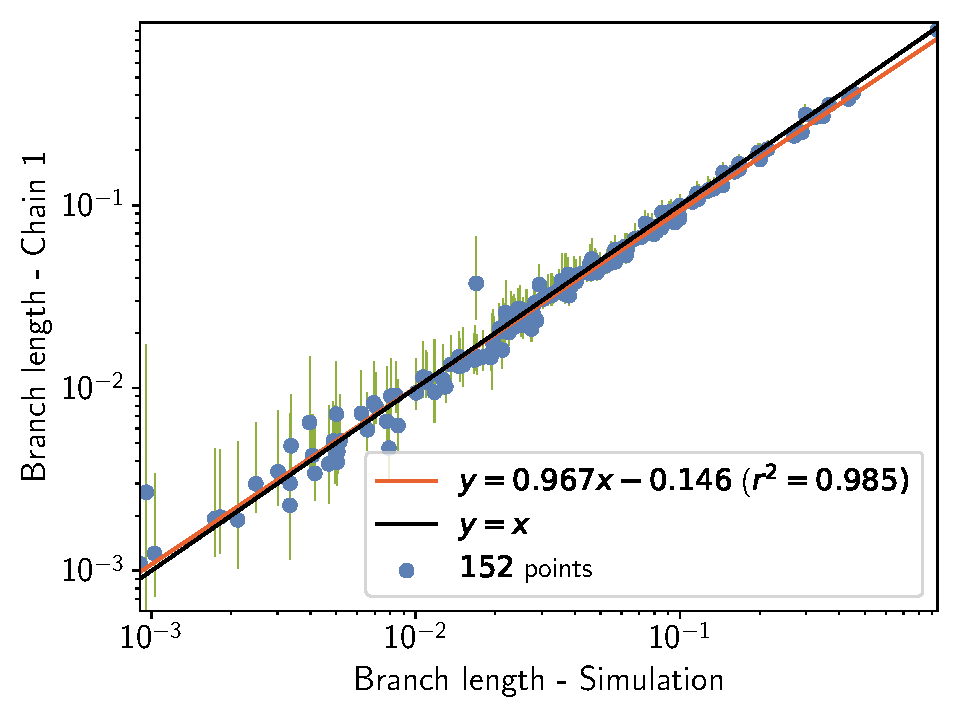
\includegraphics[width=\linewidth, page=1]{simulations/SimuFold_SiteMutSelBranchNe_BranchCorrelation_Log10BranchLength}
    \end{minipage} \hfill
    \begin{minipage}{0.32\linewidth}
        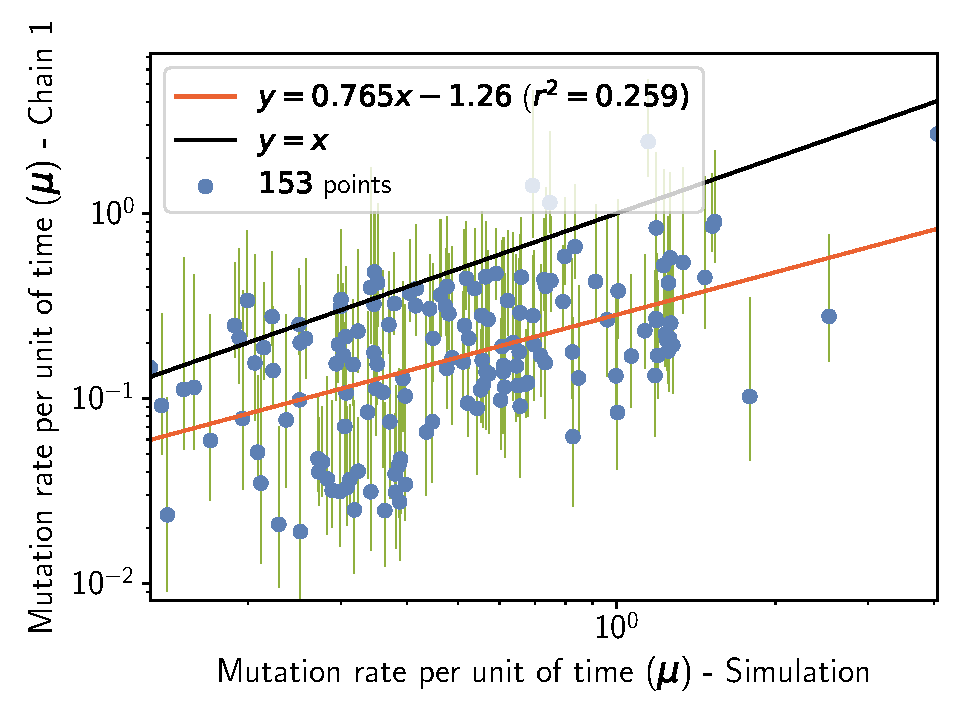
\includegraphics[width=\linewidth, page=1]{simulations/SimuFold_SiteMutSelBranchNe_BranchCorrelation_LogMutationRatePerTime}
    \end{minipage} \hfill
    \begin{minipage}{0.32\linewidth}
        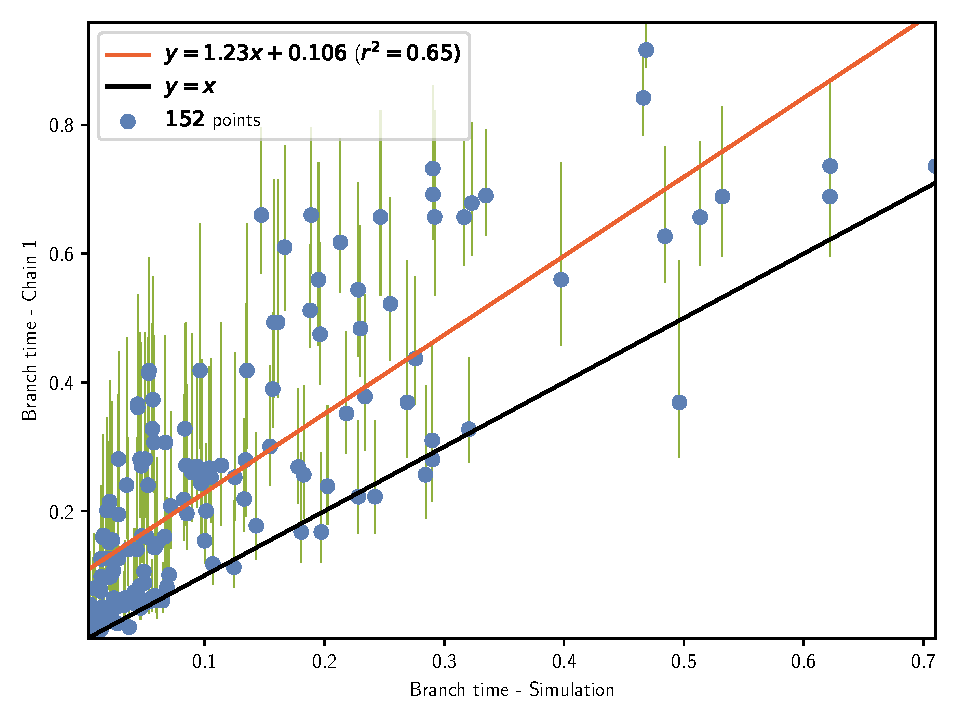
\includegraphics[width=\linewidth, page=1]{simulations/SimuFold_SiteMutSelBranchNe_BranchCorrelation_BranchTime}
    \end{minipage} \hfill
    \begin{minipage}{0.32\linewidth}
        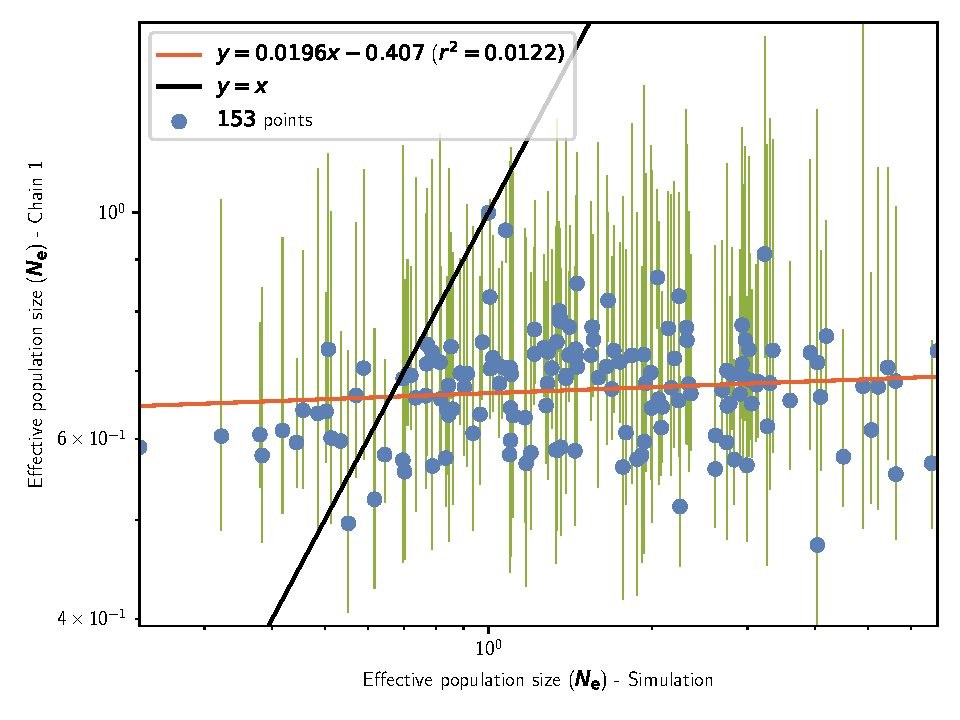
\includegraphics[width=\linewidth, page=1]{simulations/SimuFold_SiteMutSelBranchNe_BranchCorrelation_LogPopulationSize}
    \end{minipage}
    \begin{minipage}{0.32\linewidth}
        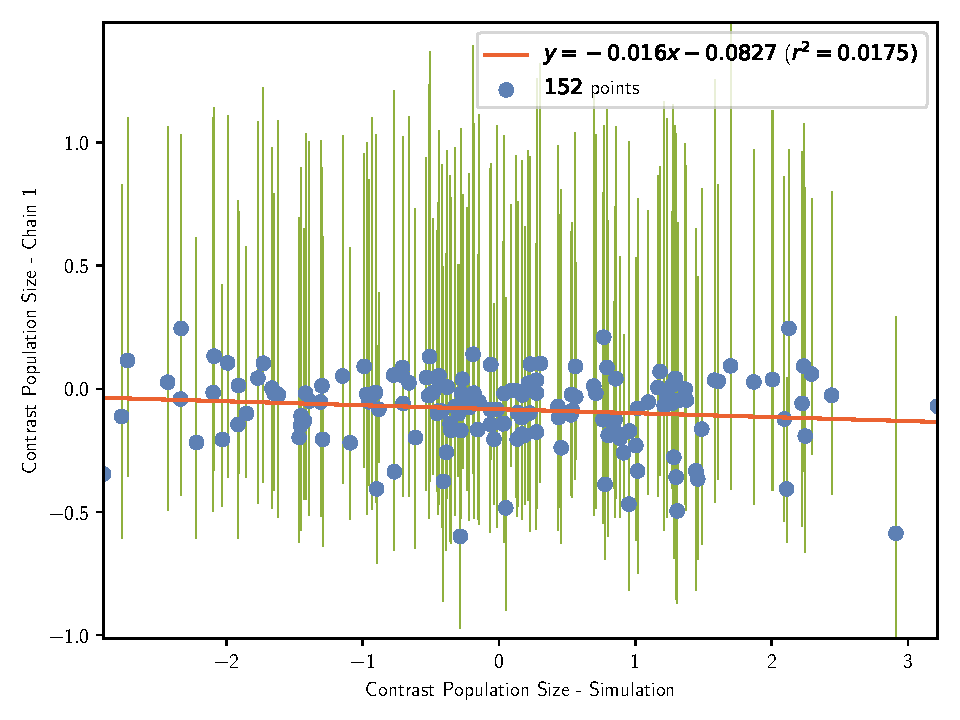
\includegraphics[width=\linewidth, page=1]{simulations/SimuFold_SiteMutSelBranchNe_BranchCorrelation_ContrastPopulationSize}
    \end{minipage} \hfill
    \caption[Inferred branch parameters for SimuFold]{
    Inferred branch parameters under simulation accounting for site epistasis (folding stability model), thus fluctuation of the selection coefficient along the phylogeny.
    }
\end{figure}

\begin{table}[H]
    \centering
    \noindent\adjustbox{max width=\textwidth}{%
    \begin{tabu}{|c|c|c|}
        \hline
        \textbf{Experiment} & $\langle \entropy \rangle$ (\textbf{branch} $\Ne$) & $\langle \entropy \rangle$ (\textbf{constant} $\Ne$) \\ \hline
        \hline
        SimuFold, chain~1 & $1.31 \pm 0.05$ & $1.61 \pm 0.03$\\ \hline
        SimuFold, chain 2 & $1.30 \pm 0.04$ & $1.60 \pm 0.03$\\ \hline
    \end{tabu}}
    \caption[Amino-acid entropy in SimuFold]{
    Estimated amino-acid entropy under simulation accounting for site epistasis (folding stability model), thus fluctuation of the selection coefficient along the phylogeny.
    Obtained with the inference model of site selection for amino acid, and branch fluctuation of $\Ne$ (left column), or under the assumption of constant $\Ne$ (right column)}
\end{table}


\section{Empirical data in mammals}
\label{sec:empirical-data-in-mammals}

\subsection{Chain convergence}
\label{subsec:chain-convergence}
Obtained with the inference model of site selection for amino acid, and branch fluctuation of $\Ne$.

\begin{figure}[H]
    \centering
    \begin{minipage}{0.49\linewidth}
        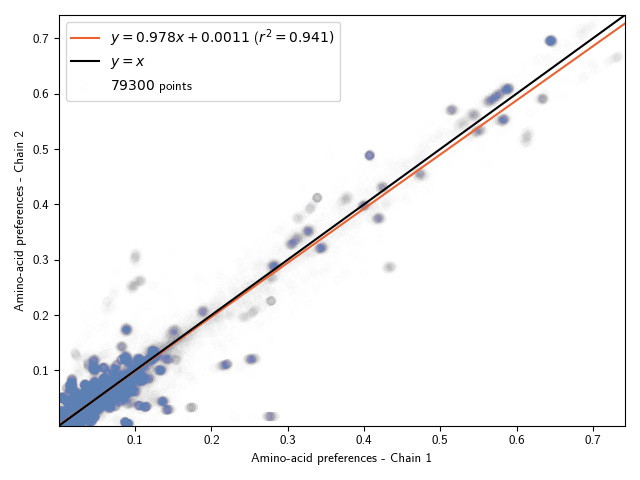
\includegraphics[width=\linewidth, page=1]{mammals/18CDS_SiteMutSelBranchNe_R1_ProfileCorrelation.png}
    \end{minipage} \hfill
    \begin{minipage}{0.49\linewidth}
        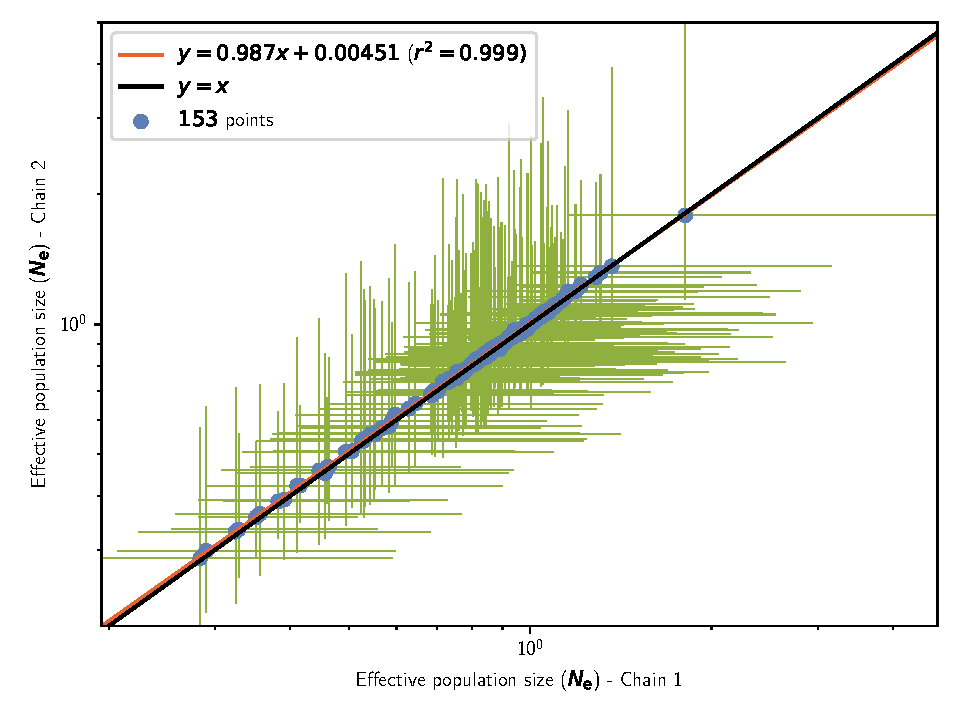
\includegraphics[width=\linewidth, page=1]{mammals/18CDS_SiteMutSelBranchNe_R1_LogPopulationSizeCorrelation}
    \end{minipage}
    \caption[Chain convergence of site profiles and branche $\Ne$]{
    Chain convergence of site amino-acid preferences (left panel) and branch $\Ne$ (right panel).}
\end{figure}

\subsection{Traits estimation \& correlation (replicate~1, chain~1)}
Obtained with the inference model of site selection for amino acid, and branch fluctuation of $\Ne$.

\begin{table}[H]
    \centering
\noindent\adjustbox{max width=\textwidth}{%
\begin{tabu}{|c||c|c|c|c|c|}
\hline
\textbf{Covariance ($\bm{\Sigma}$)} & $\bm{N_{\text{e}}}$ & $\bm{\mu}$ & \textbf{Maximum longevity } & \textbf{Adult weight } & \textbf{Female maturity }\\
\hhline{|=#=|=|=|=|=|}
$\bm{N_{\text{e}}}$ & $0.281^{**}$ & $0.324^{**}$ & $-0.268^{**}$ & $-1.29^{**}$ & $-0.308^{**}$\\\hline
$\bm{\mu}$ & - & $1.93^{**}$ & $-1.12^{**}$ & $-5.19^{**}$ & $-1.43^{**}$\\\hline
\textbf{Maximum longevity } & - & - & $0.934^{**}$ & $3.58^{**}$ & $1.01^{**}$\\\hline
\textbf{Adult weight } & - & - & - & $19.9^{**}$ & $4.48^{**}$\\\hline
\textbf{Female maturity } & - & - & - & - & $1.53^{**}$\\\hline
\end{tabu}}

    \caption[Covariance matrix in mammals]{
    Covariance coefficient between effective population size~($\Ne$), mutation rate per site per unit of time~($\mu$), and life-history traits (maximum longevity, adult weight and female maturity) were computed in placental mammals.
    Asterisks indicate strength of support ($\smash{^{*}} pp > 0.95$, $\smash{^{**}} pp > 0.975$).}
\end{table}

\begin{table}[H]
    \centering
\noindent\adjustbox{max width=\textwidth}{%
\begin{tabu}{|c||c|c|c|c|c|}
\hline
\textbf{Partial coefficient} & $\bm{N_{\mathrm{e}}}$ & $\bm{\mu}$ & \textbf{Maximum longevity } & \textbf{Adult weight } & \textbf{Female maturity }\\
\hhline{|=#=|=|=|=|=|}
$\bm{N_{\mathrm{e}}}$ & - & $-0.146$ & $-0.177$ & $-0.265^{*}$ & $-0.0223$\\\hline
$\bm{\mu}$ & - & - & $-0.283^{*}$ & $-0.396^{**}$ & $-0.327^{**}$\\\hline
\textbf{Maximum longevity } & - & - & - & $0.236^{*}$ & $0.383^{**}$\\\hline
\textbf{Adult weight } & - & - & - & - & $0.179$\\\hline
\textbf{Female maturity } & - & - & - & - & -\\\hline
\end{tabu}}

    \caption[Partial correlation coefficient matrix in mammals]{
    Partial correlation coefficient between effective population size~($\Ne$), mutation rate per site per unit of time~($\mu$), and life-history traits (maximum longevity, adult weight and female maturity) were computed in placental mammals.
    Asterisks indicate strength of support ($\smash{^{*}} pp > 0.95$, $\smash{^{**}} pp > 0.975$).}
    \label{tab:table-partcor-mammals}
\end{table}

\begin{figure}[H]
    \centering
    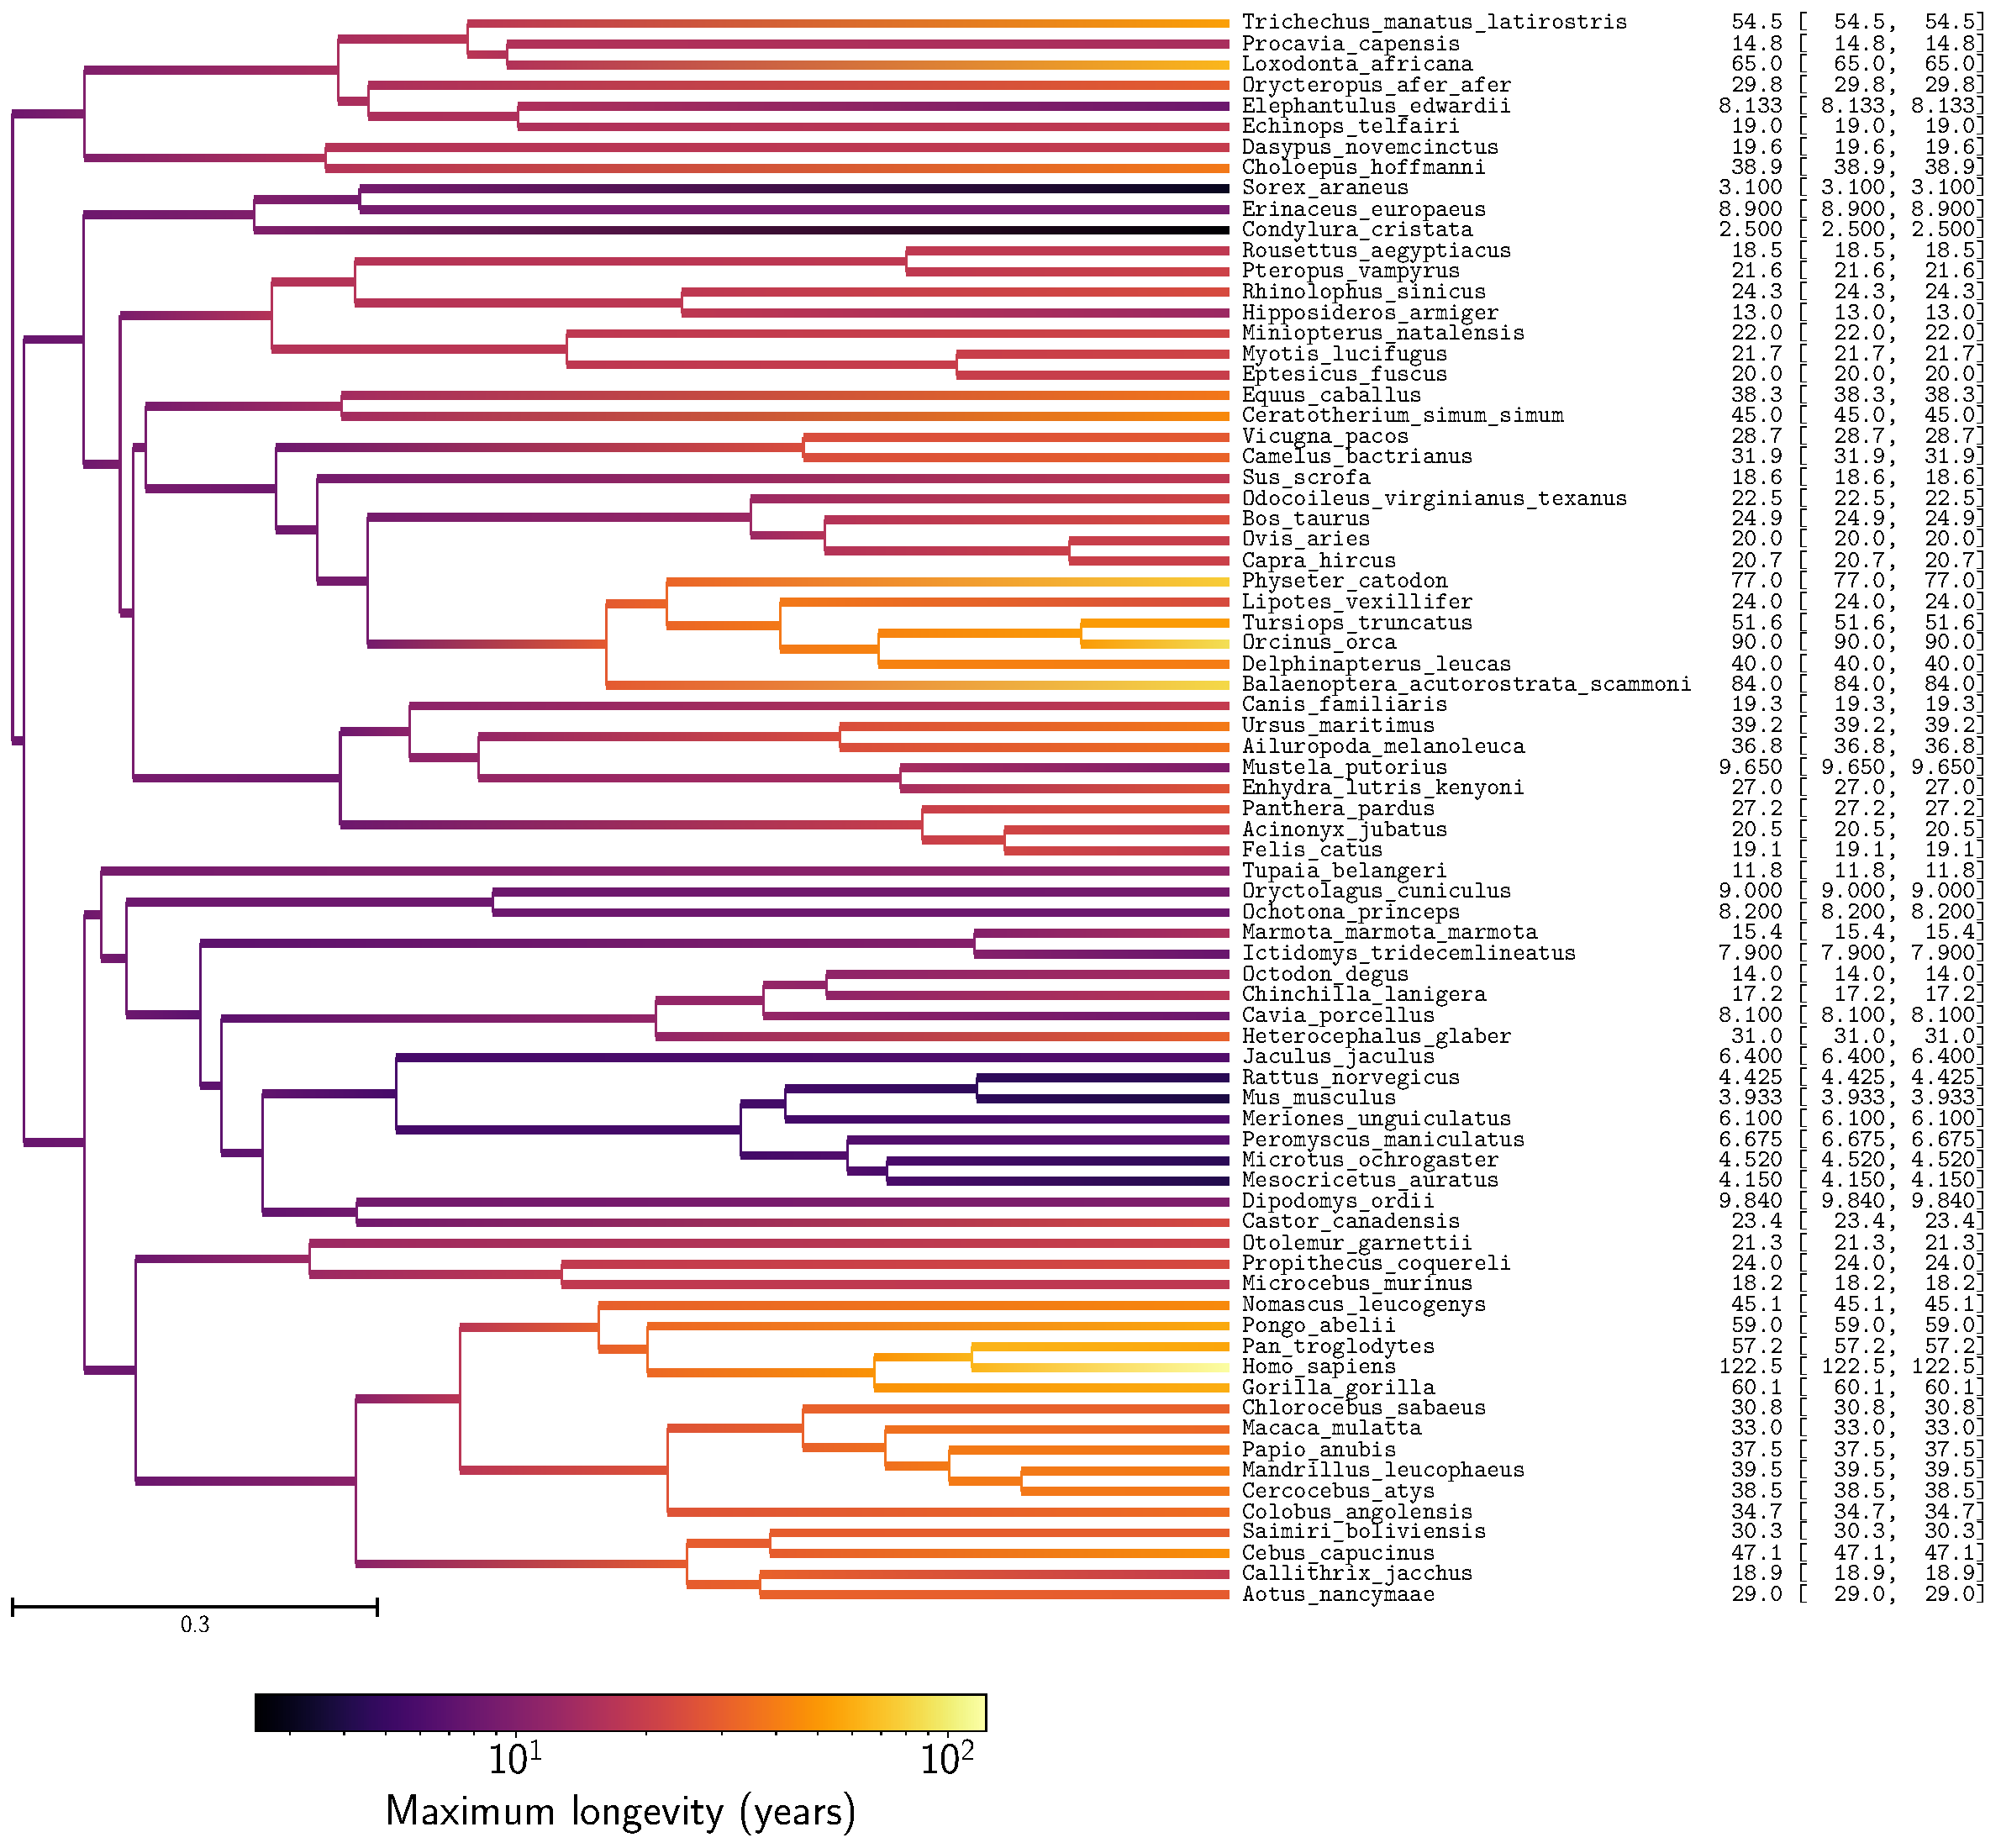
\includegraphics[width=\linewidth, page=1]{mammals/18CDS_SiteMutSelBranchNe_R1_LogMaximum_longevity}
    \caption[Maximum longevity estimation in mammals]{Maximum longevity estimation in mammals}
\end{figure}

\begin{figure}[H]
    \centering
    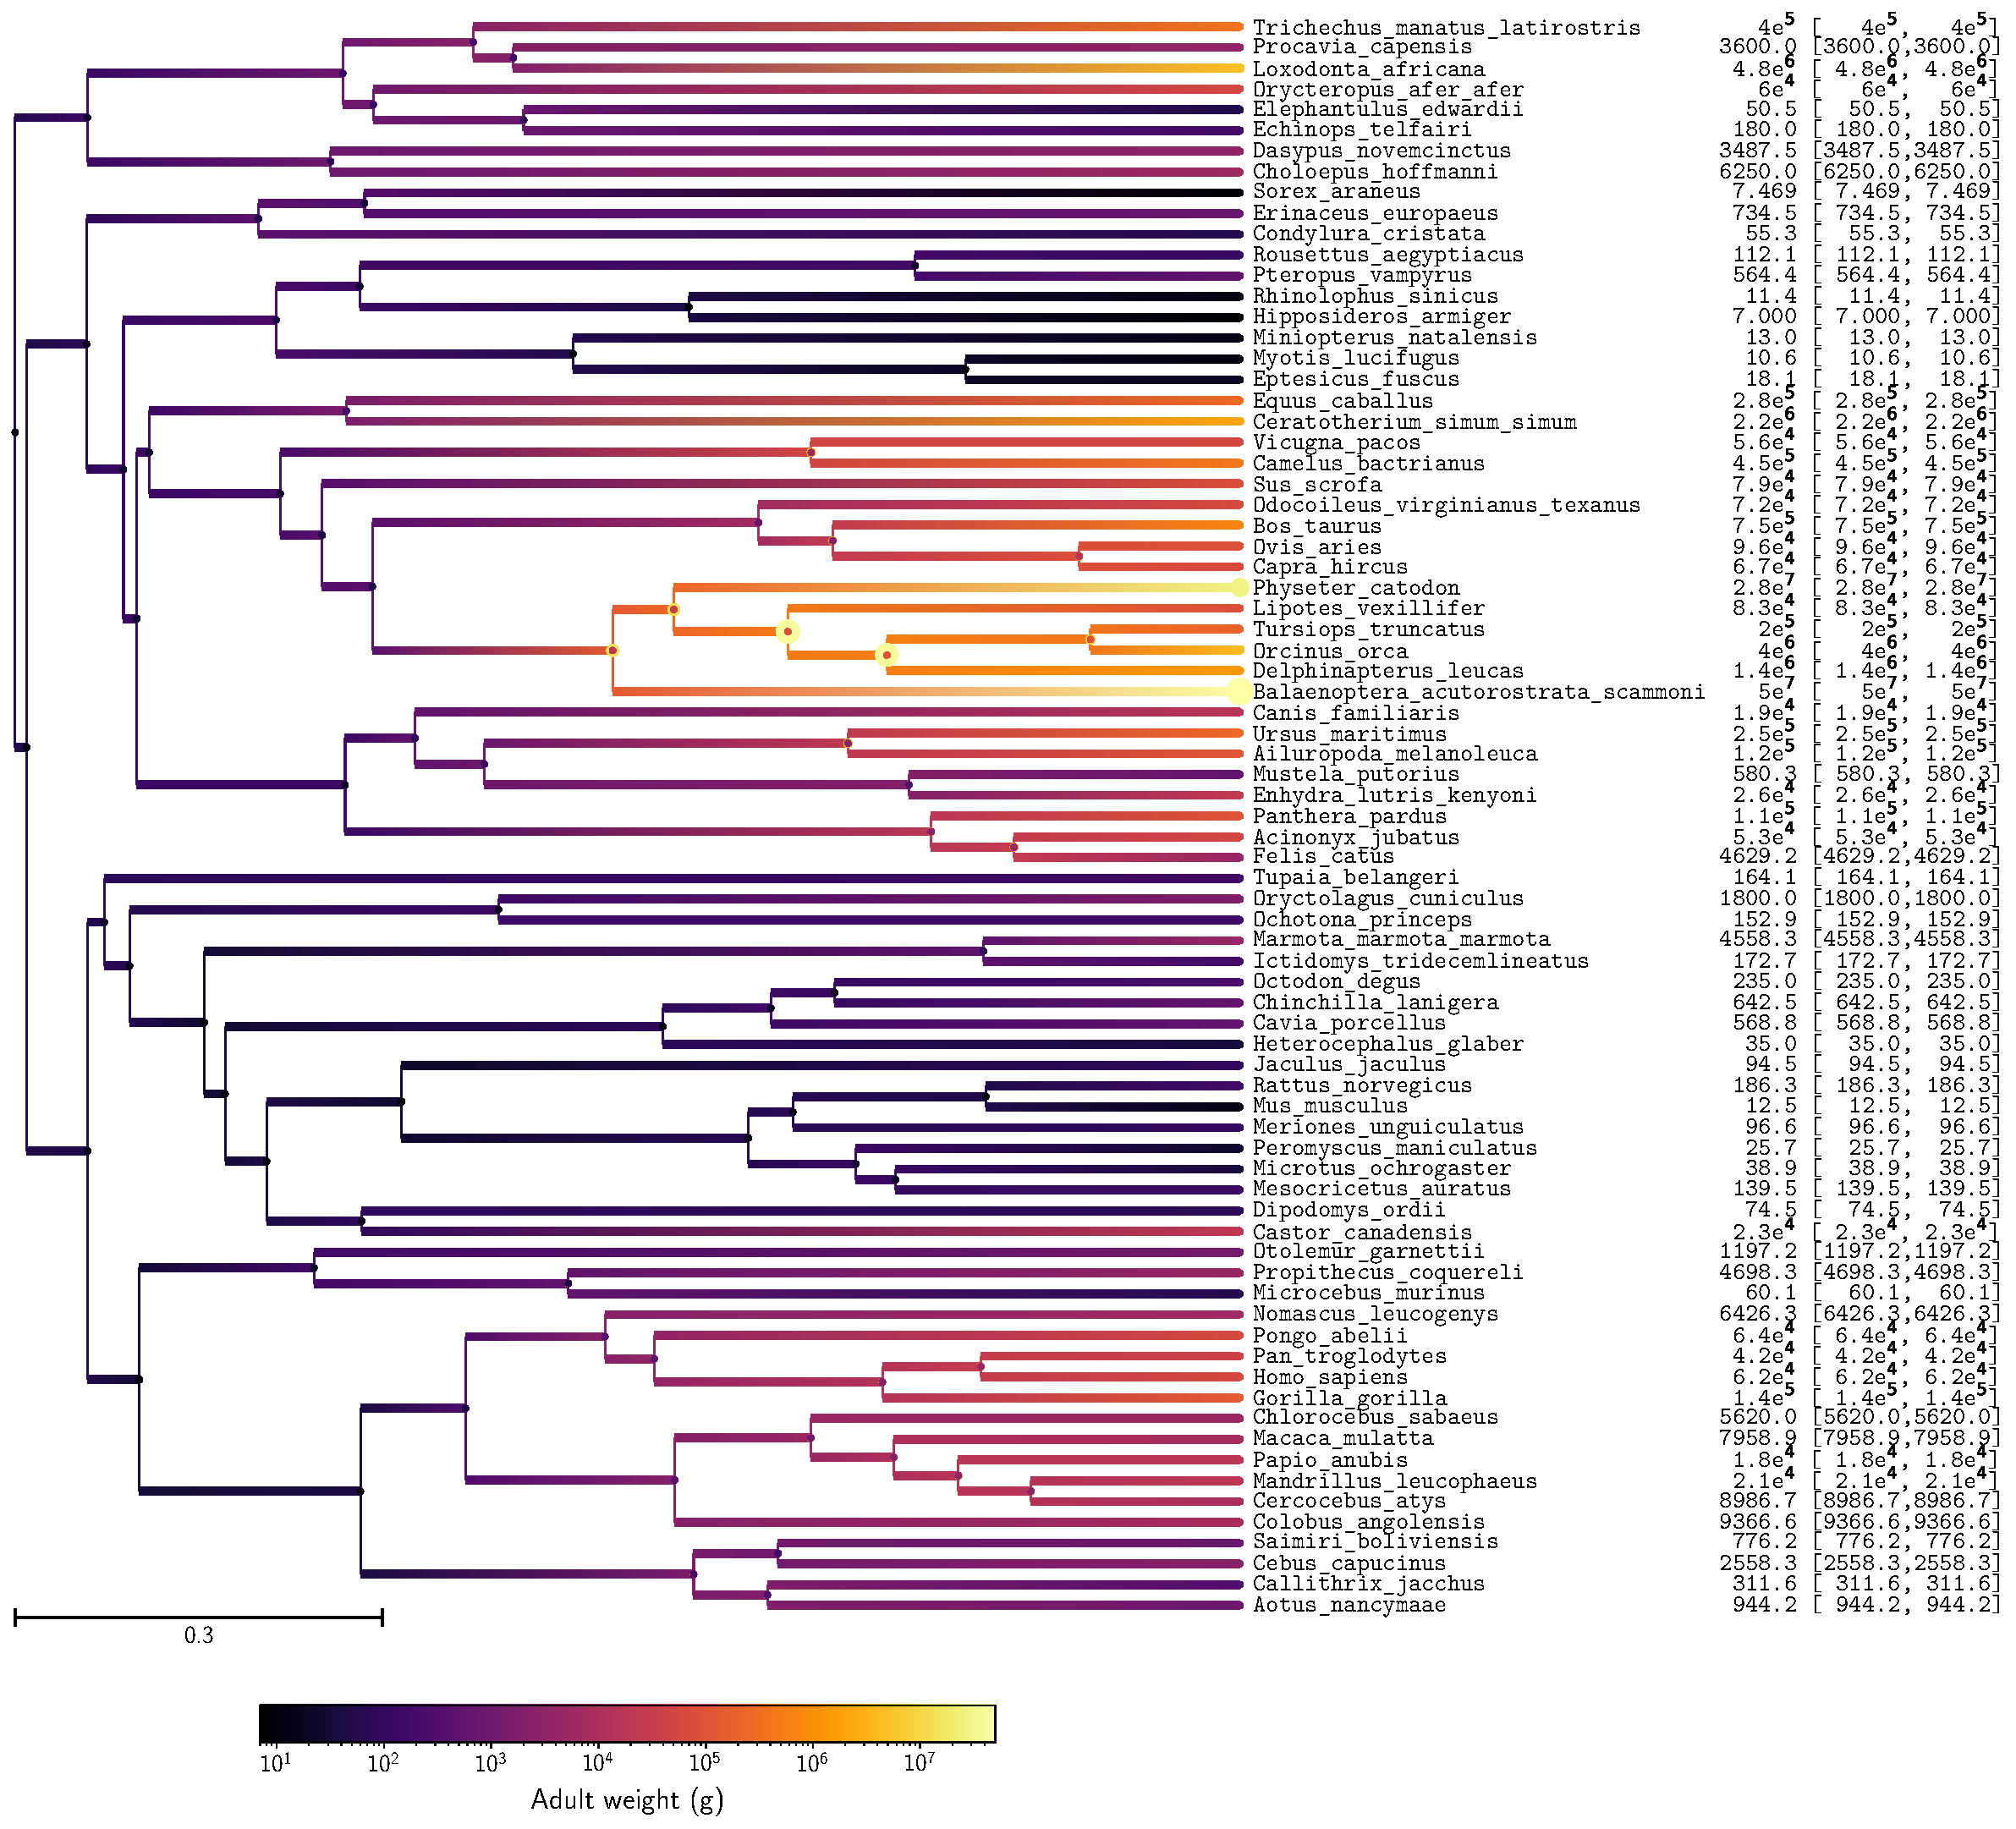
\includegraphics[width=\linewidth, page=1]{mammals/18CDS_SiteMutSelBranchNe_R1_LogAdult_weight}
    \caption[Adult weight estimation in mammals]{Adult weight estimation in mammals}
\end{figure}

\begin{figure}[H]
    \centering
    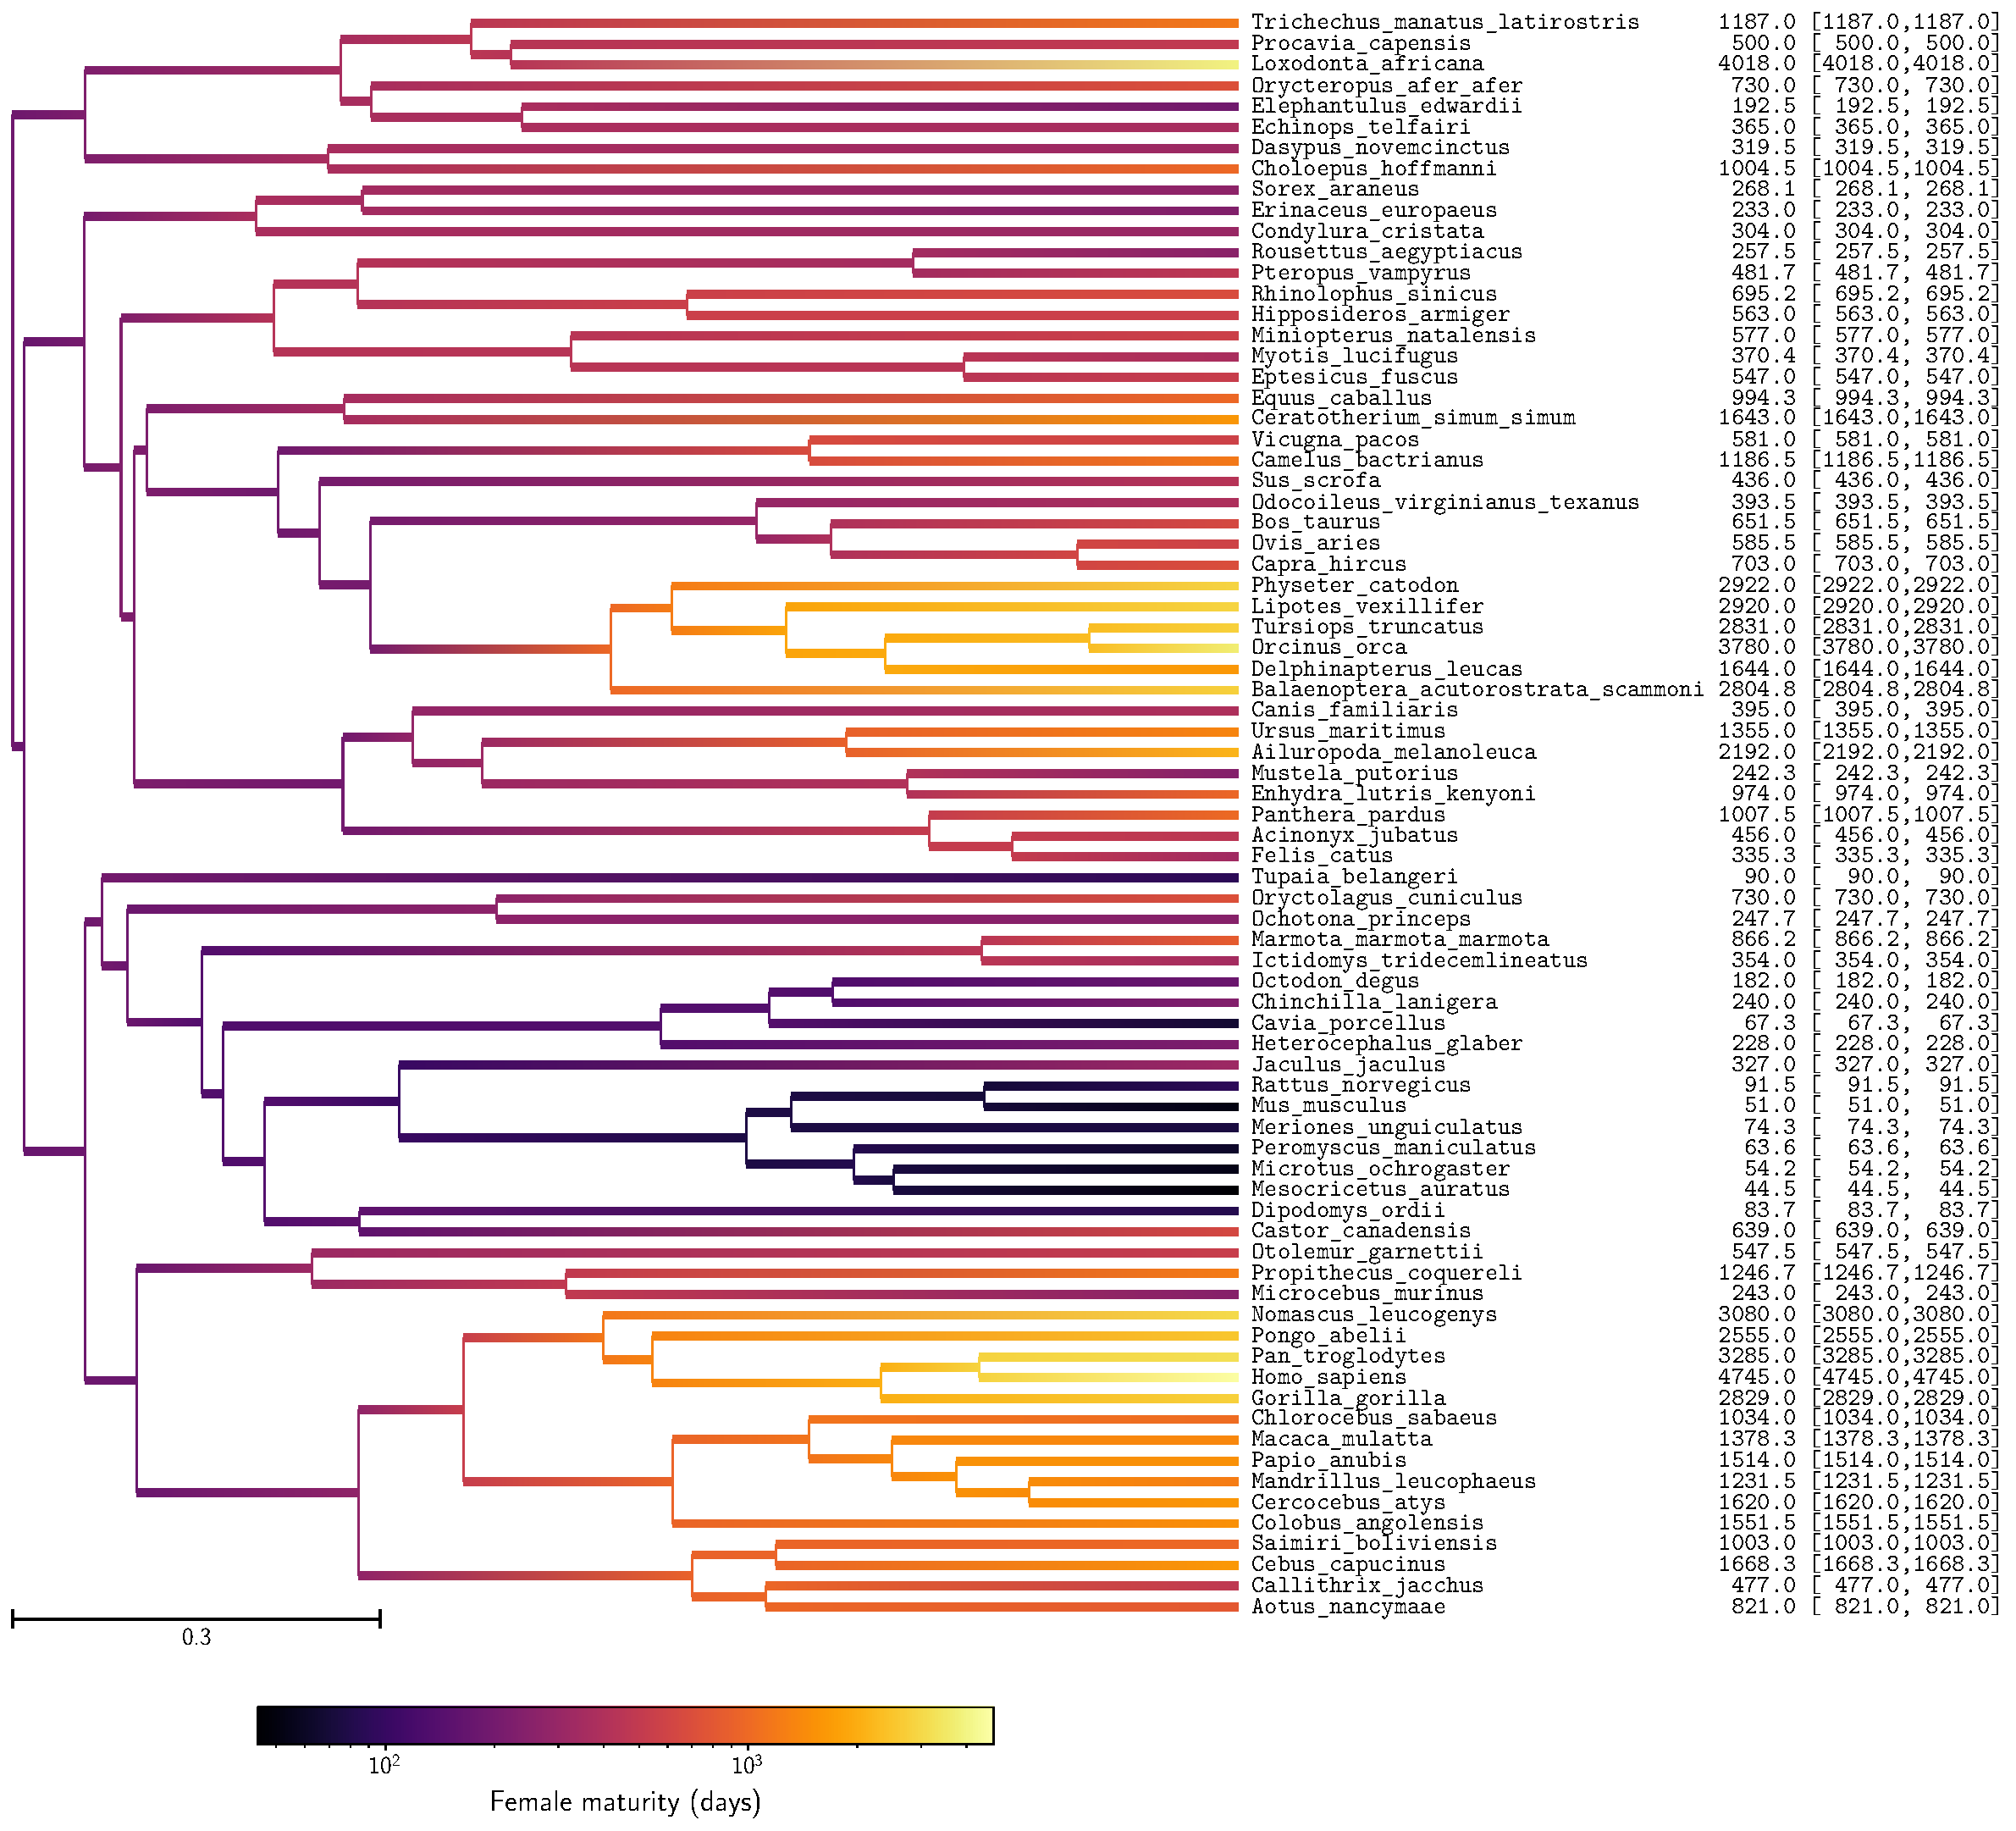
\includegraphics[width=\linewidth, page=1]{mammals/18CDS_SiteMutSelBranchNe_R1_LogFemale_maturity}
    \caption[Female maturity estimation in mammals]{Female maturity estimation in mammals}
\end{figure}

\subsection{Repeatability of experiments}
Obtained with the inference model of site selection for amino acid, and branch fluctuation of $\Ne$.

\begin{figure}[H]
    \centering
    \begin{minipage}{0.32\linewidth}
        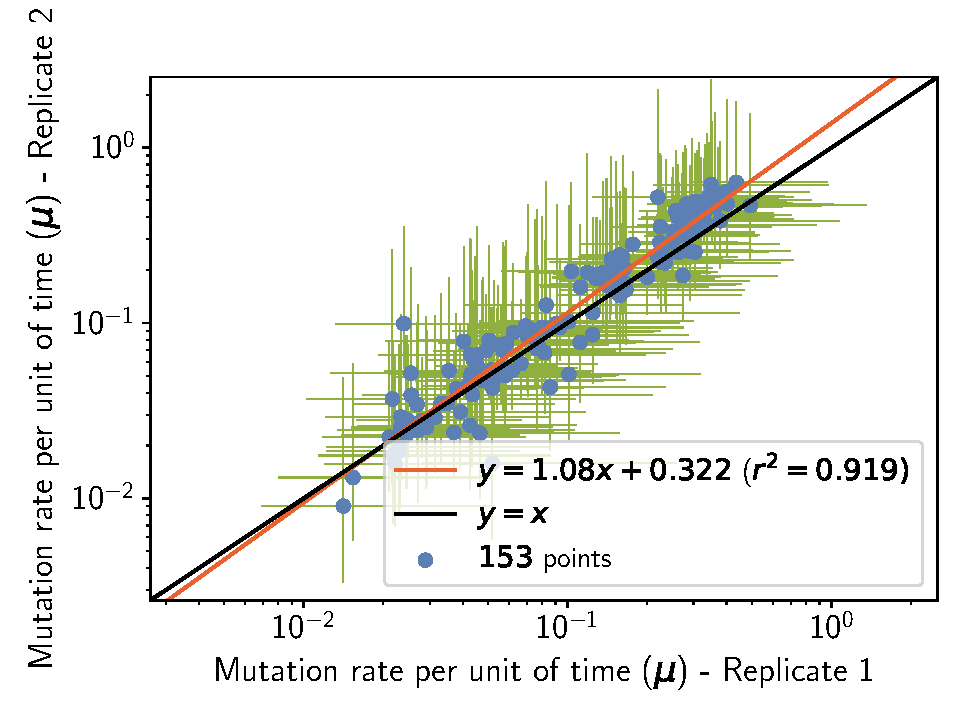
\includegraphics[width=\linewidth, page=1]{mammals/18CDS_SiteMutSelBranchNe_Rep_LogMutationRatePerTime-1-2}
    \end{minipage} \hfill
    \begin{minipage}{0.32\linewidth}
        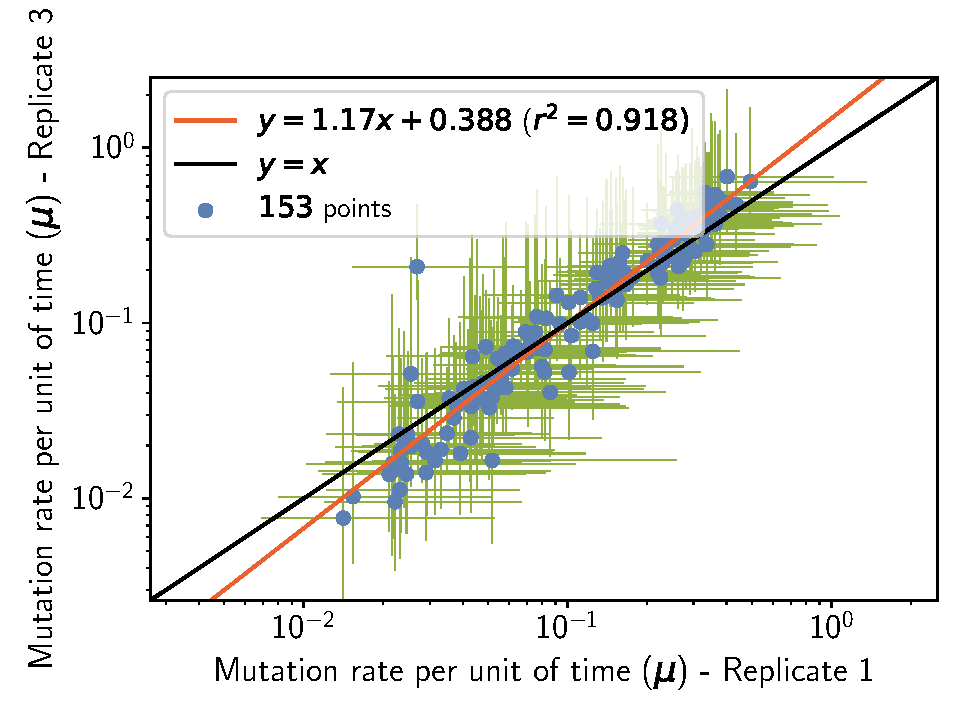
\includegraphics[width=\linewidth, page=1]{mammals/18CDS_SiteMutSelBranchNe_Rep_LogMutationRatePerTime-1-3}
    \end{minipage} \hfill
    \begin{minipage}{0.32\linewidth}
        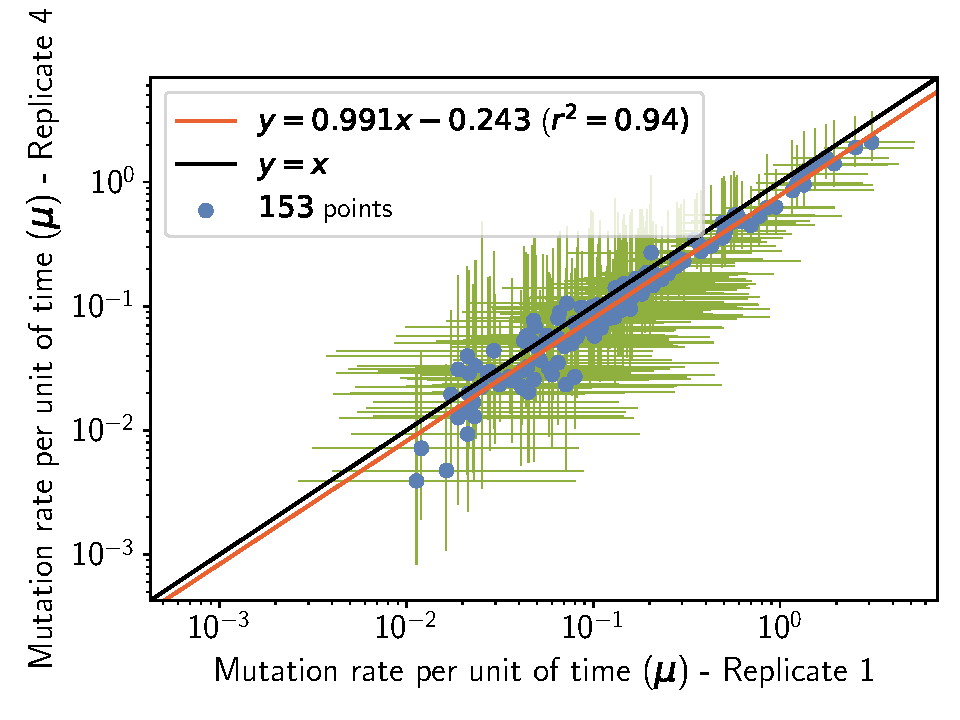
\includegraphics[width=\linewidth, page=1]{mammals/18CDS_SiteMutSelBranchNe_Rep_LogMutationRatePerTime-1-4}
    \end{minipage}
    \caption[Repeatability of mutation rate estimation in mammals]{Repeatability of mutation rate ($\mu$) estimation in mammals}
\end{figure}

\begin{figure}[H]
    \centering
    \begin{minipage}{0.32\linewidth}
        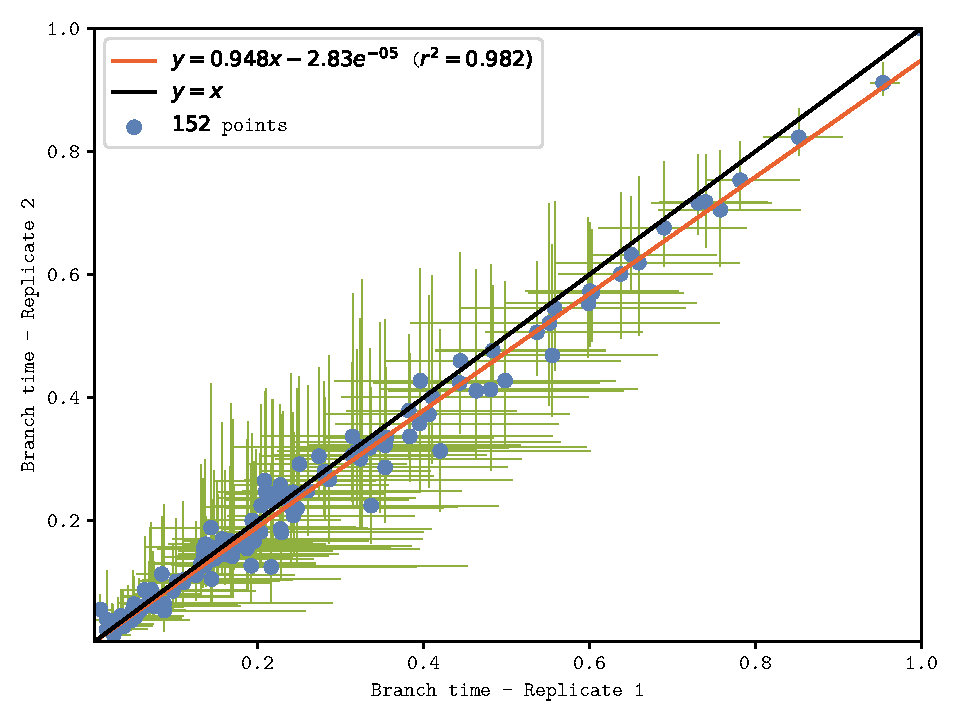
\includegraphics[width=\linewidth, page=1]{mammals/18CDS_SiteMutSelBranchNe_Rep_BranchTime-1-2}
    \end{minipage} \hfill
    \begin{minipage}{0.32\linewidth}
        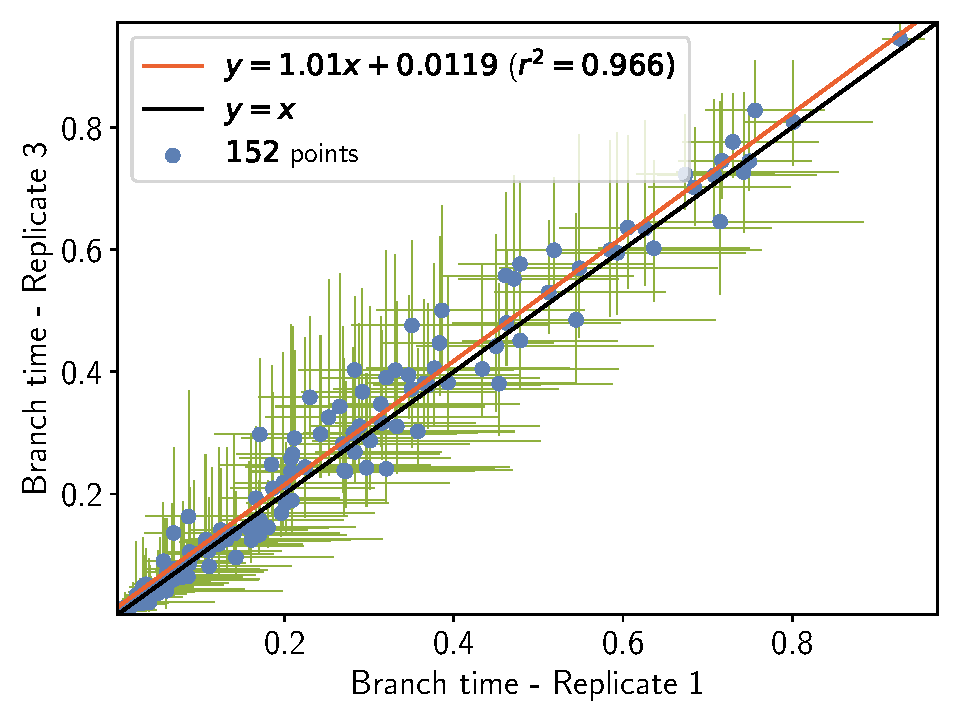
\includegraphics[width=\linewidth, page=1]{mammals/18CDS_SiteMutSelBranchNe_Rep_BranchTime-1-3}
    \end{minipage} \hfill
    \begin{minipage}{0.32\linewidth}
        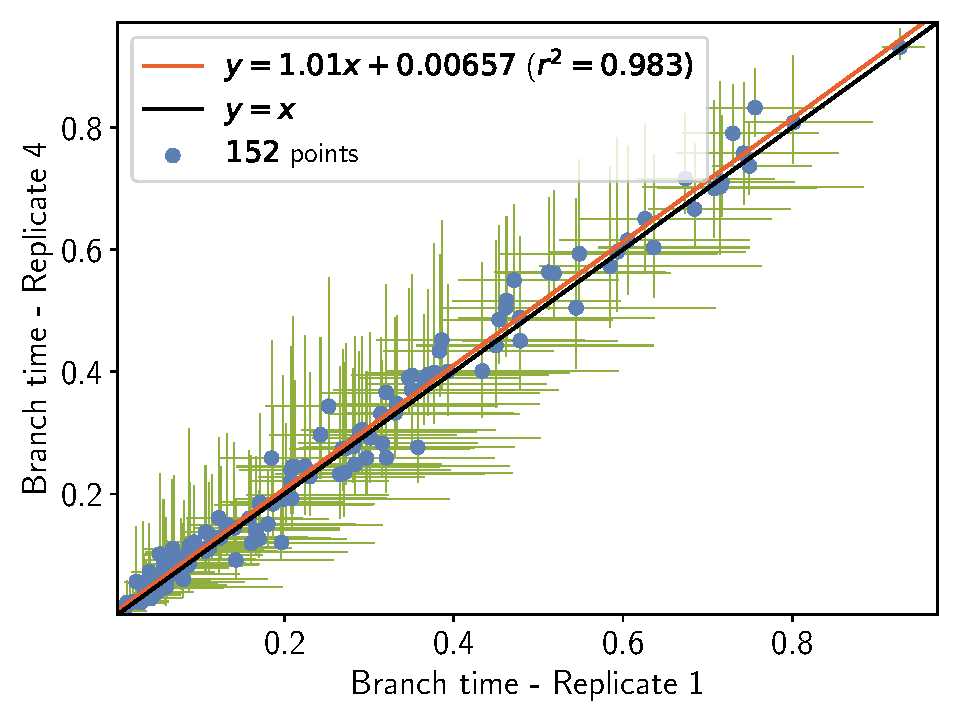
\includegraphics[width=\linewidth, page=1]{mammals/18CDS_SiteMutSelBranchNe_Rep_BranchTime-1-4}
    \end{minipage}
    \caption[Repeatability of branch time estimation in mammals]{Repeatability of branch time ($\Delta T$) estimation in mammals}
\end{figure}

\begin{table}[H]
    \centering
\noindent\adjustbox{max width=\textwidth}{%
\begin{tabu}{|c||c|c|c|}
\hline
\textbf{Correlation ($\bm{\rho}$)} & $\bm{N_{\mathrm{e}}}$ & $\bm{\mu}$ & \textbf{LogGenomeSize}\\
\hhline{|=#=|=|=|}
$\bm{N_{\mathrm{e}}}$ & - & $-0.0623$ & $-0.144$\\\hline
$\bm{\mu}$ & - & - & $0.224$\\\hline
\textbf{LogGenomeSize} & - & - & -\\\hline
\end{tabu}}
 \\
    \centering
\noindent\adjustbox{max width=\textwidth}{%
\begin{tabu}{|c||c|c|c|c|c|}
\hline
\textbf{Correlation ($\bm{\rho}$)} & $\bm{N_{\mathrm{e}}}$ & $\bm{\mu}$ & \textbf{Maximum longevity } & \textbf{Adult weight } & \textbf{Female maturity }\\
\hhline{|=#=|=|=|=|=|}
$\bm{N_{\mathrm{e}}}$ & - & $0.51^{**}$ & $-0.591^{**}$ & $-0.496^{**}$ & $-0.465^{**}$\\\hline
$\bm{\mu}$ & - & - & $-0.771^{**}$ & $-0.722^{**}$ & $-0.679^{**}$\\\hline
\textbf{Maximum longevity } & - & - & - & $0.802^{**}$ & $0.812^{**}$\\\hline
\textbf{Adult weight } & - & - & - & - & $0.764^{**}$\\\hline
\textbf{Female maturity } & - & - & - & - & -\\\hline
\end{tabu}}
 \\
    \centering
\noindent\adjustbox{max width=\textwidth}{%
\begin{tabu}{|c||c|c|c|}
\hline
\textbf{Correlation ($\bm{\rho}$)} & $\bm{N_{\mathrm{e}}}$ & $\bm{\mu}$ & \textbf{LogGenomeSize}\\
\hhline{|=#=|=|=|}
$\bm{N_{\mathrm{e}}}$ & - & $0.0479$ & $-0.158$\\\hline
$\bm{\mu}$ & - & - & $0.173$\\\hline
\textbf{LogGenomeSize} & - & - & -\\\hline
\end{tabu}}
 \\
    \centering
\noindent\adjustbox{max width=\textwidth}{%
\begin{tabu}{|c||c|c|c|}
\hline
\textbf{Correlation ($\bm{\rho}$)} & $\bm{N_{\mathrm{e}}}$ & $\bm{\mu}$ & \textbf{LogGenomeSize}\\
\hhline{|=#=|=|=|}
$\bm{N_{\mathrm{e}}}$ & - & $-0.0355$ & $-0.0875$\\\hline
$\bm{\mu}$ & - & - & $0.225$\\\hline
\textbf{LogGenomeSize} & - & - & -\\\hline
\end{tabu}}

    \caption[Covariance matrix repeatability in mammals]{
    In all four replicates, covariance coefficient between effective population size~($\Ne$), mutation rate per site per unit of time~($\mu$), and life-history traits (maximum longevity, adult weight and female maturity) were computed in placental mammals.
    Asterisks indicate strength of support ($\smash{^{*}} pp > 0.95$, $\smash{^{**}} pp > 0.975$).}
\end{table}

\subsection{Amino-acid preferences entropy}

\begin{table}[H]
    \centering
    \noindent\adjustbox{max width=\textwidth}{%
    \begin{tabu}{|c|c|c|}
        \hline
        \textbf{Experiment} & $\langle \entropy \rangle$ (\textbf{branch} $\Ne$) & $\langle \entropy \rangle$ (\textbf{constant} $\Ne$) \\ \hline
        \hline
        Mammals 18 CDS, replicate~1, Chain 1 & $1.07 \pm 0.10$ & $1.14 \pm 0.10$\\ \hline
        Mammals 18 CDS, replicate 2, Chain 2 & $1.07 \pm 0.09$ & $1.14 \pm 0.10$\\ \hline
        Mammals 18 CDS, replicate 2, Chain 1 & $1.06 \pm 0.10$ & $1.12 \pm 0.09$\\ \hline
        Mammals 18 CDS, replicate 2, Chain 2 & $1.06 \pm 0.09$ & $1.11 \pm 0.10$\\ \hline
        Mammals 18 CDS, replicate 3, Chain 1 & $1.08 \pm 0.12$ & $1.15 \pm 0.11$\\ \hline
        Mammals 18 CDS, replicate 3, Chain 2 & $1.04 \pm 0.10$ & $1.18 \pm 0.11$\\ \hline
        Mammals 18 CDS, replicate 4, Chain 1 & $0.94 \pm 0.11$ & $1.02 \pm 0.12$\\ \hline
        Mammals 18 CDS, replicate 4, Chain 2 & $0.89 \pm 0.11$ & $1.02 \pm 0.11$\\ \hline
        \hline
        Mammals 36 CDS, replicate~1, Chain 1 & $1.02 \pm 0.06$ & $1.07 \pm 0.10$\\ \hline
        Mammals 36 CDS, replicate~1, Chain 2 & $0.91 \pm 0.07$ & $1.03 \pm 0.07$\\ \hline
        Mammals 36 CDS, replicate 2, Chain 1 & $0.92 \pm 0.09$ & $0.96 \pm 0.09$\\ \hline
        Mammals 36 CDS, replicate 2, Chain 2 & $1.01 \pm 0.09$ & $1.02 \pm 0.11$\\ \hline
        Mammals 36 CDS, replicate 3, Chain 1 & $0.93 \pm 0.00$ & $1.05 \pm 0.09$\\ \hline
        Mammals 36 CDS, replicate 3, Chain 2 & $1.02 \pm 0.07$ & $1.05 \pm 0.11$\\ \hline
        Mammals 36 CDS, replicate 4, Chain 1 & $1.04 \pm 0.07$ & $1.10 \pm 0.08$\\ \hline
        Mammals 36 CDS, replicate 4, Chain 2 & $1.03 \pm 0.10$ & $1.08 \pm 0.08$\\ \hline
        Mammals 36 CDS, replicate 5, Chain 1 & $1.03 \pm 0.10$ & $1.03 \pm 0.08$\\ \hline
        Mammals 36 CDS, replicate 5, Chain 2 & $0.99 \pm 0.10$ & $1.04 \pm 0.08$\\ \hline
        Mammals 36 CDS, replicate 6, Chain 1 & $1.05 \pm 0.10$ & $1.10 \pm 0.08$\\ \hline
        Mammals 36 CDS, replicate 6, Chain 2 & $0.97 \pm 0.11$ & $1.10 \pm 0.10$\\ \hline
    \end{tabu}}
    \caption[Entropy of amino acids in mammals]{Estimated amino acids entropy in mammals.
    Obtained with the inference model of site selection for amino acid, and branch fluctuation of $\Ne$ (left column), or under the assumption of constant $\Ne$ (right column)}
    \label{tab:table-entropy-aa-mutselne}
\end{table}

\subsection{Traits estimation with branch \texorpdfstring{$\omega$}{ω} (replicate~1, chain~1)}
Obtained with the model of branch fluctuation of $\dnds$ (without site selection for amino acid).

\begin{figure}[H]
    \centering
    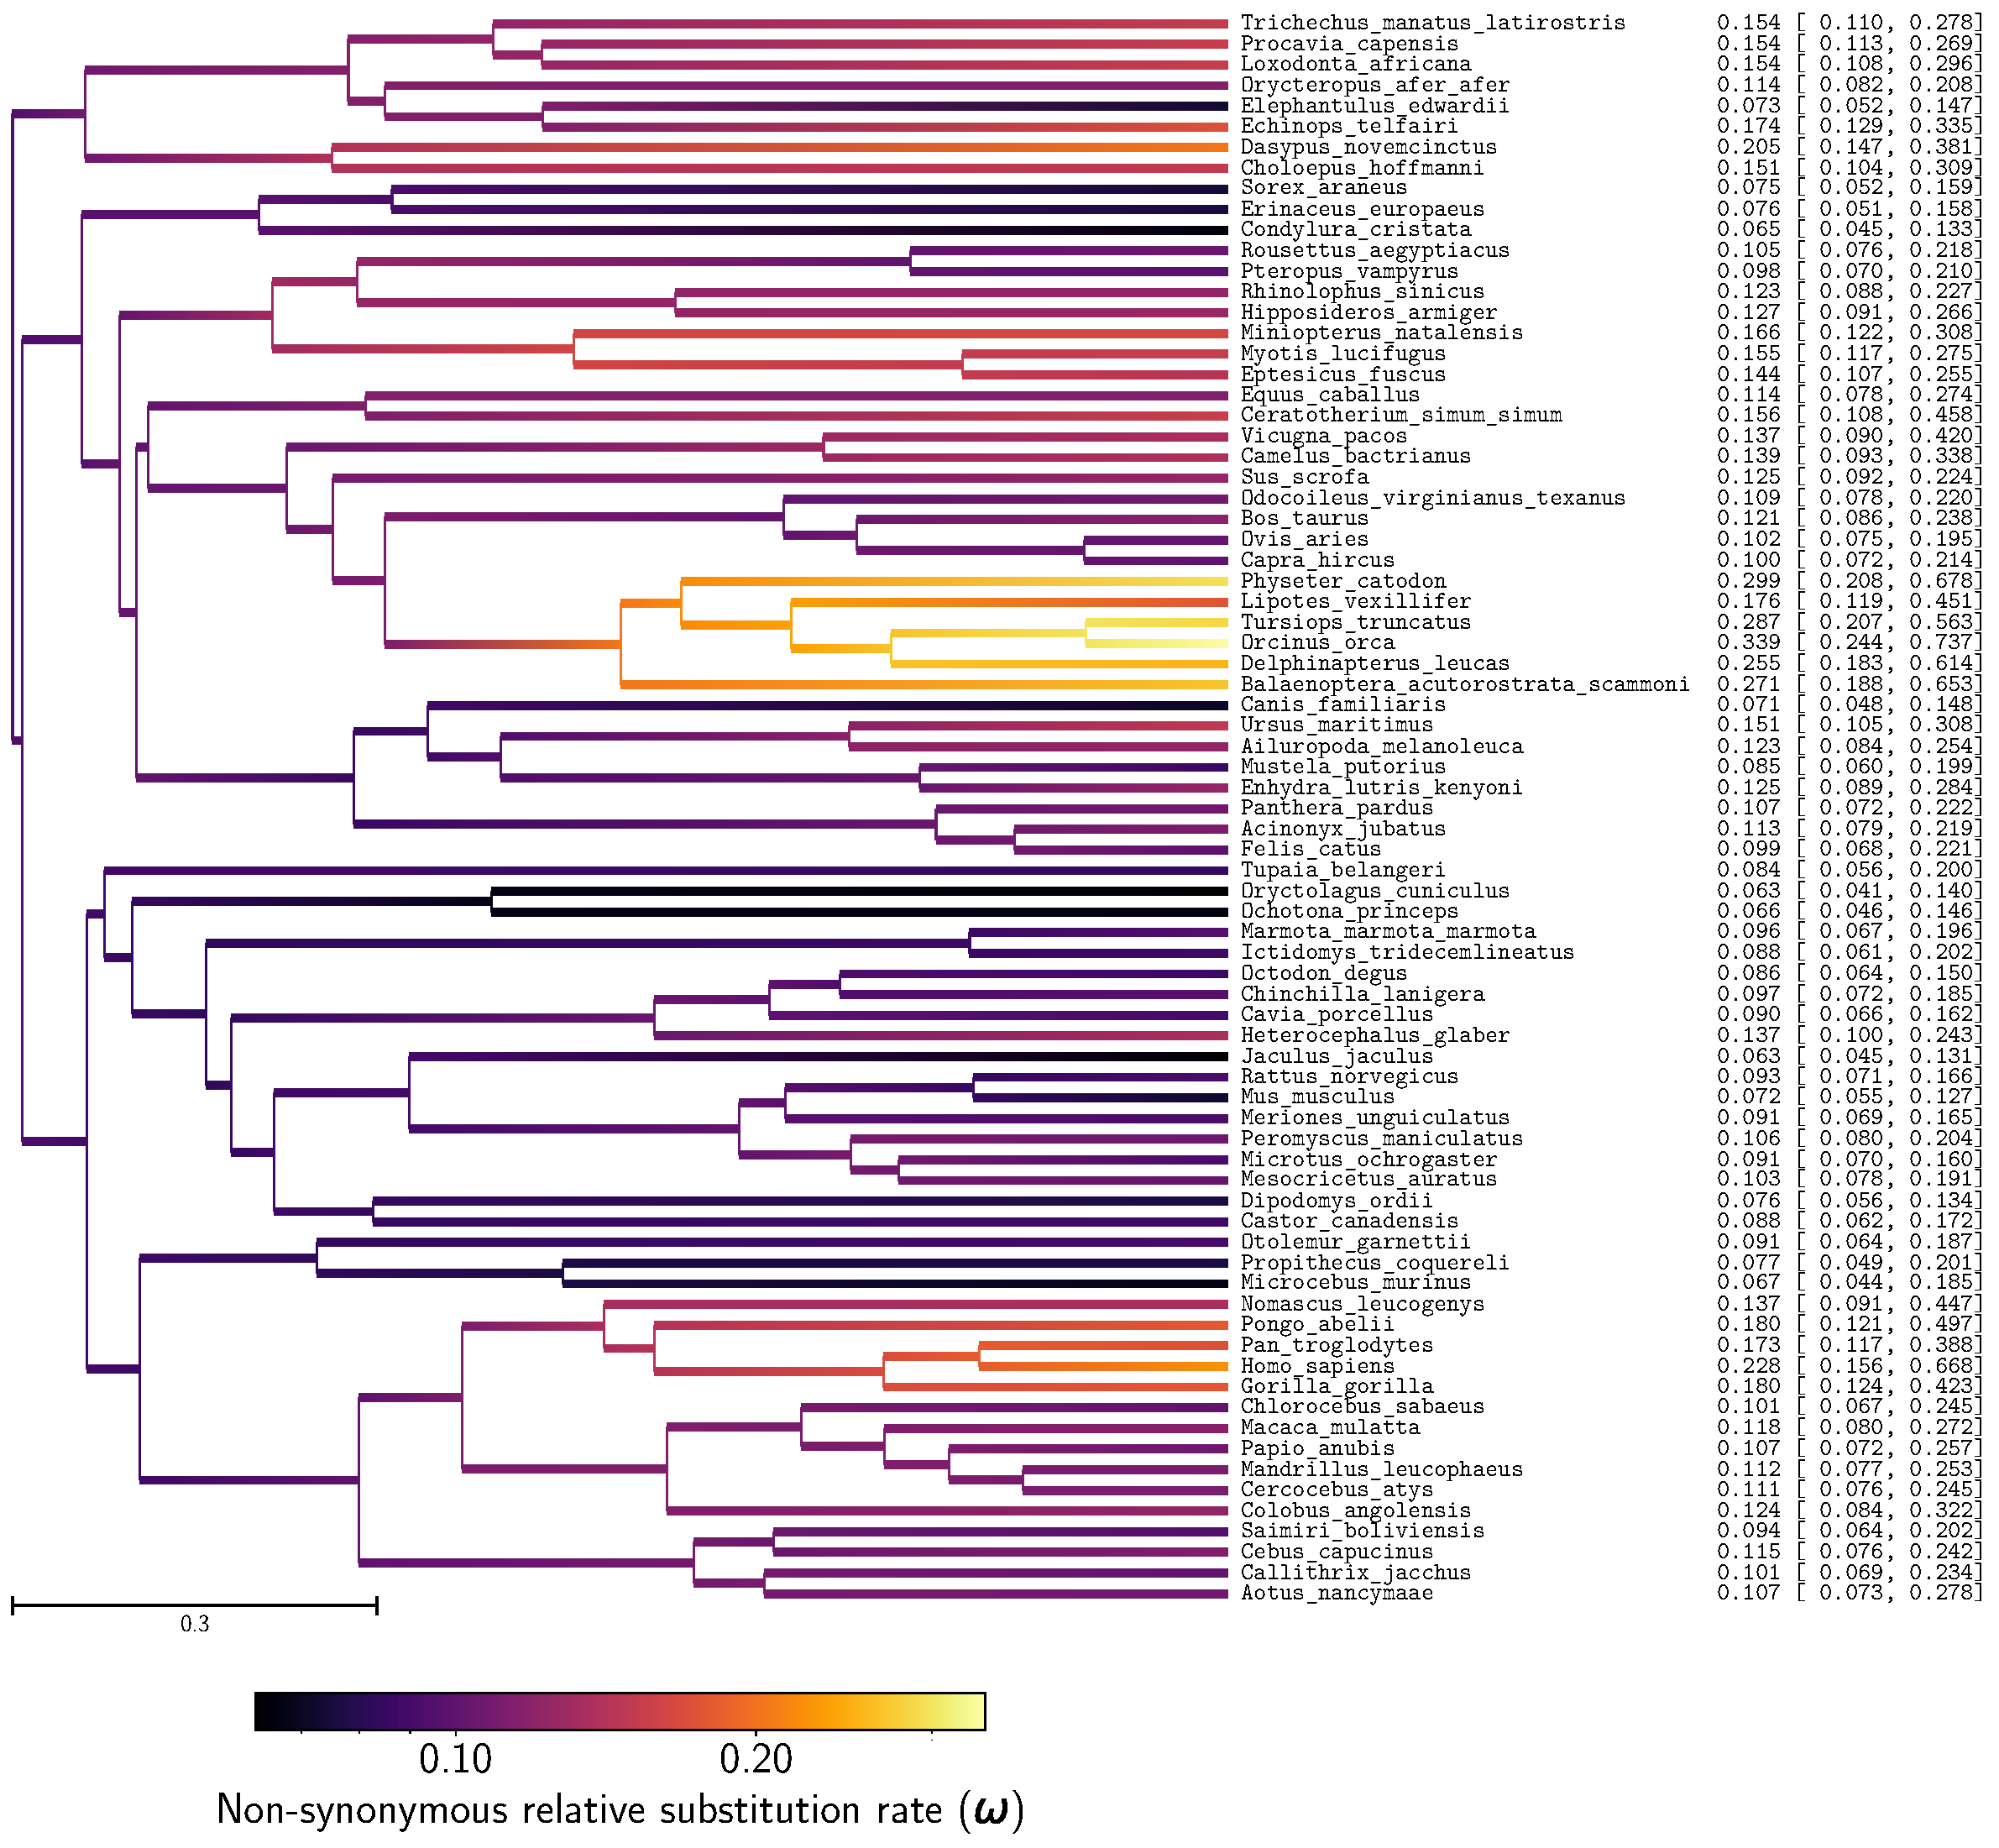
\includegraphics[width=\linewidth, page=1]{mammals/18CDS_BranchOmega_R1_LogdNdS}
    \caption[$\dnds$ estimation in mammals]{{Non-synonymous substitution} rate ($\dnds$) estimation in mammals}
\end{figure}

\begin{table}[H]
    \centering
\noindent\adjustbox{max width=\textwidth}{%
\begin{tabu}{|c||c|c|c|}
\hline
\textbf{Correlation ($\bm{\rho}$)} & $\bm{\omega}$ & $\bm{\mu}$ & \textbf{LogGenomeSize}\\
\hhline{|=#=|=|=|}
$\bm{\omega}$ & - & $0.147$ & $0.152$\\\hline
$\bm{\mu}$ & - & - & $0.251$\\\hline
\textbf{LogGenomeSize} & - & - & -\\\hline
\end{tabu}}

    \caption[Correlation coefficient matrix in mammals ($\dnds$)]{
    Correlation coefficient between non-synonymous substitution rate~($\dnds$), mutation rate per site per unit of time~($\mu$), and life-history traits (maximum longevity, adult weight and female maturity) were computed in placental mammals.
    Asterisks indicate strength of support ($\smash{^{*}} pp > 0.95$, $\smash{^{**}} pp > 0.975$).}
\end{table}

\begin{table}[H]
    \centering
\noindent\adjustbox{max width=\textwidth}{%
\begin{tabu}{|c||c|c|c|c|c|}
\hline
\textbf{Covariance ($\bm{\Sigma}$)} & $\bm{\omega}$ & $\bm{\mu}$ & \textbf{Maximum longevity } & \textbf{Adult weight } & \textbf{Female maturity }\\
\hhline{|=#=|=|=|=|=|}
$\bm{\omega}$ & $0.215^{**}$ & $-0.236^{**}$ & $0.231^{**}$ & $0.828^{**}$ & $0.242^{**}$\\\hline
$\bm{\mu}$ & - & $1.82^{**}$ & $-0.998^{**}$ & $-4.38^{**}$ & $-1.34^{**}$\\\hline
\textbf{Maximum longevity } & - & - & $0.837^{**}$ & $3.04^{**}$ & $0.917^{**}$\\\hline
\textbf{Adult weight } & - & - & - & $17.1^{**}$ & $3.93^{**}$\\\hline
\textbf{Female maturity } & - & - & - & - & $1.45^{**}$\\\hline
\end{tabu}}

    \caption[Covariance matrix in mammals ($\dnds$)]{
    Correlation coefficient between non-synonymous substitution rate~($\dnds$), mutation rate per site per unit of time~($\mu$), and life-history traits (maximum longevity, adult weight and female maturity) were computed in placental mammals.
    Asterisks indicate strength of support ($\smash{^{*}} pp > 0.95$, $\smash{^{**}} pp > 0.975$).}
\end{table}

\begin{table}[H]
    \centering
\noindent\adjustbox{max width=\textwidth}{%
\begin{tabu}{|c||c|c|c|c|c|}
\hline
\textbf{Partial coefficient} & $\bm{\omega}$ & $\bm{\mu}$ & \textbf{Maximum longevity } & \textbf{Adult weight } & \textbf{Female maturity }\\
\hhline{|=#=|=|=|=|=|}
$\bm{\omega}$ & - & $0.15$ & $0.369^{**}$ & $0.0468$ & $0.0223$\\\hline
$\bm{\mu}$ & - & - & $-0.299^{*}$ & $-0.272$ & $-0.382^{**}$\\\hline
\textbf{Maximum longevity } & - & - & - & $0.283^{**}$ & $0.338^{**}$\\\hline
\textbf{Adult weight } & - & - & - & - & $0.21^{*}$\\\hline
\textbf{Female maturity } & - & - & - & - & -\\\hline
\end{tabu}}

    \caption[Partial correlation coefficient matrix in mammals ($\dnds$)]{
    Partial correlation coefficient between non-synonymous substitution rate~($\dnds$), mutation rate per site per unit of time~($\mu$), and life-history traits (maximum longevity, adult weight and female maturity) were computed in placental mammals.
    Asterisks indicate strength of support ($\smash{^{*}} pp > 0.95$, $\smash{^{**}} pp > 0.975$).}
\end{table}


\section{Empirical data in Isopods}
\label{sec:empirical-data-in-isopods}

\subsection{Traits estimation (replicate~1, chain~1)}
Obtained with the inference model of site selection for amino acid, and branch fluctuation of $\Ne$.

\begin{figure}[H]
    \centering
    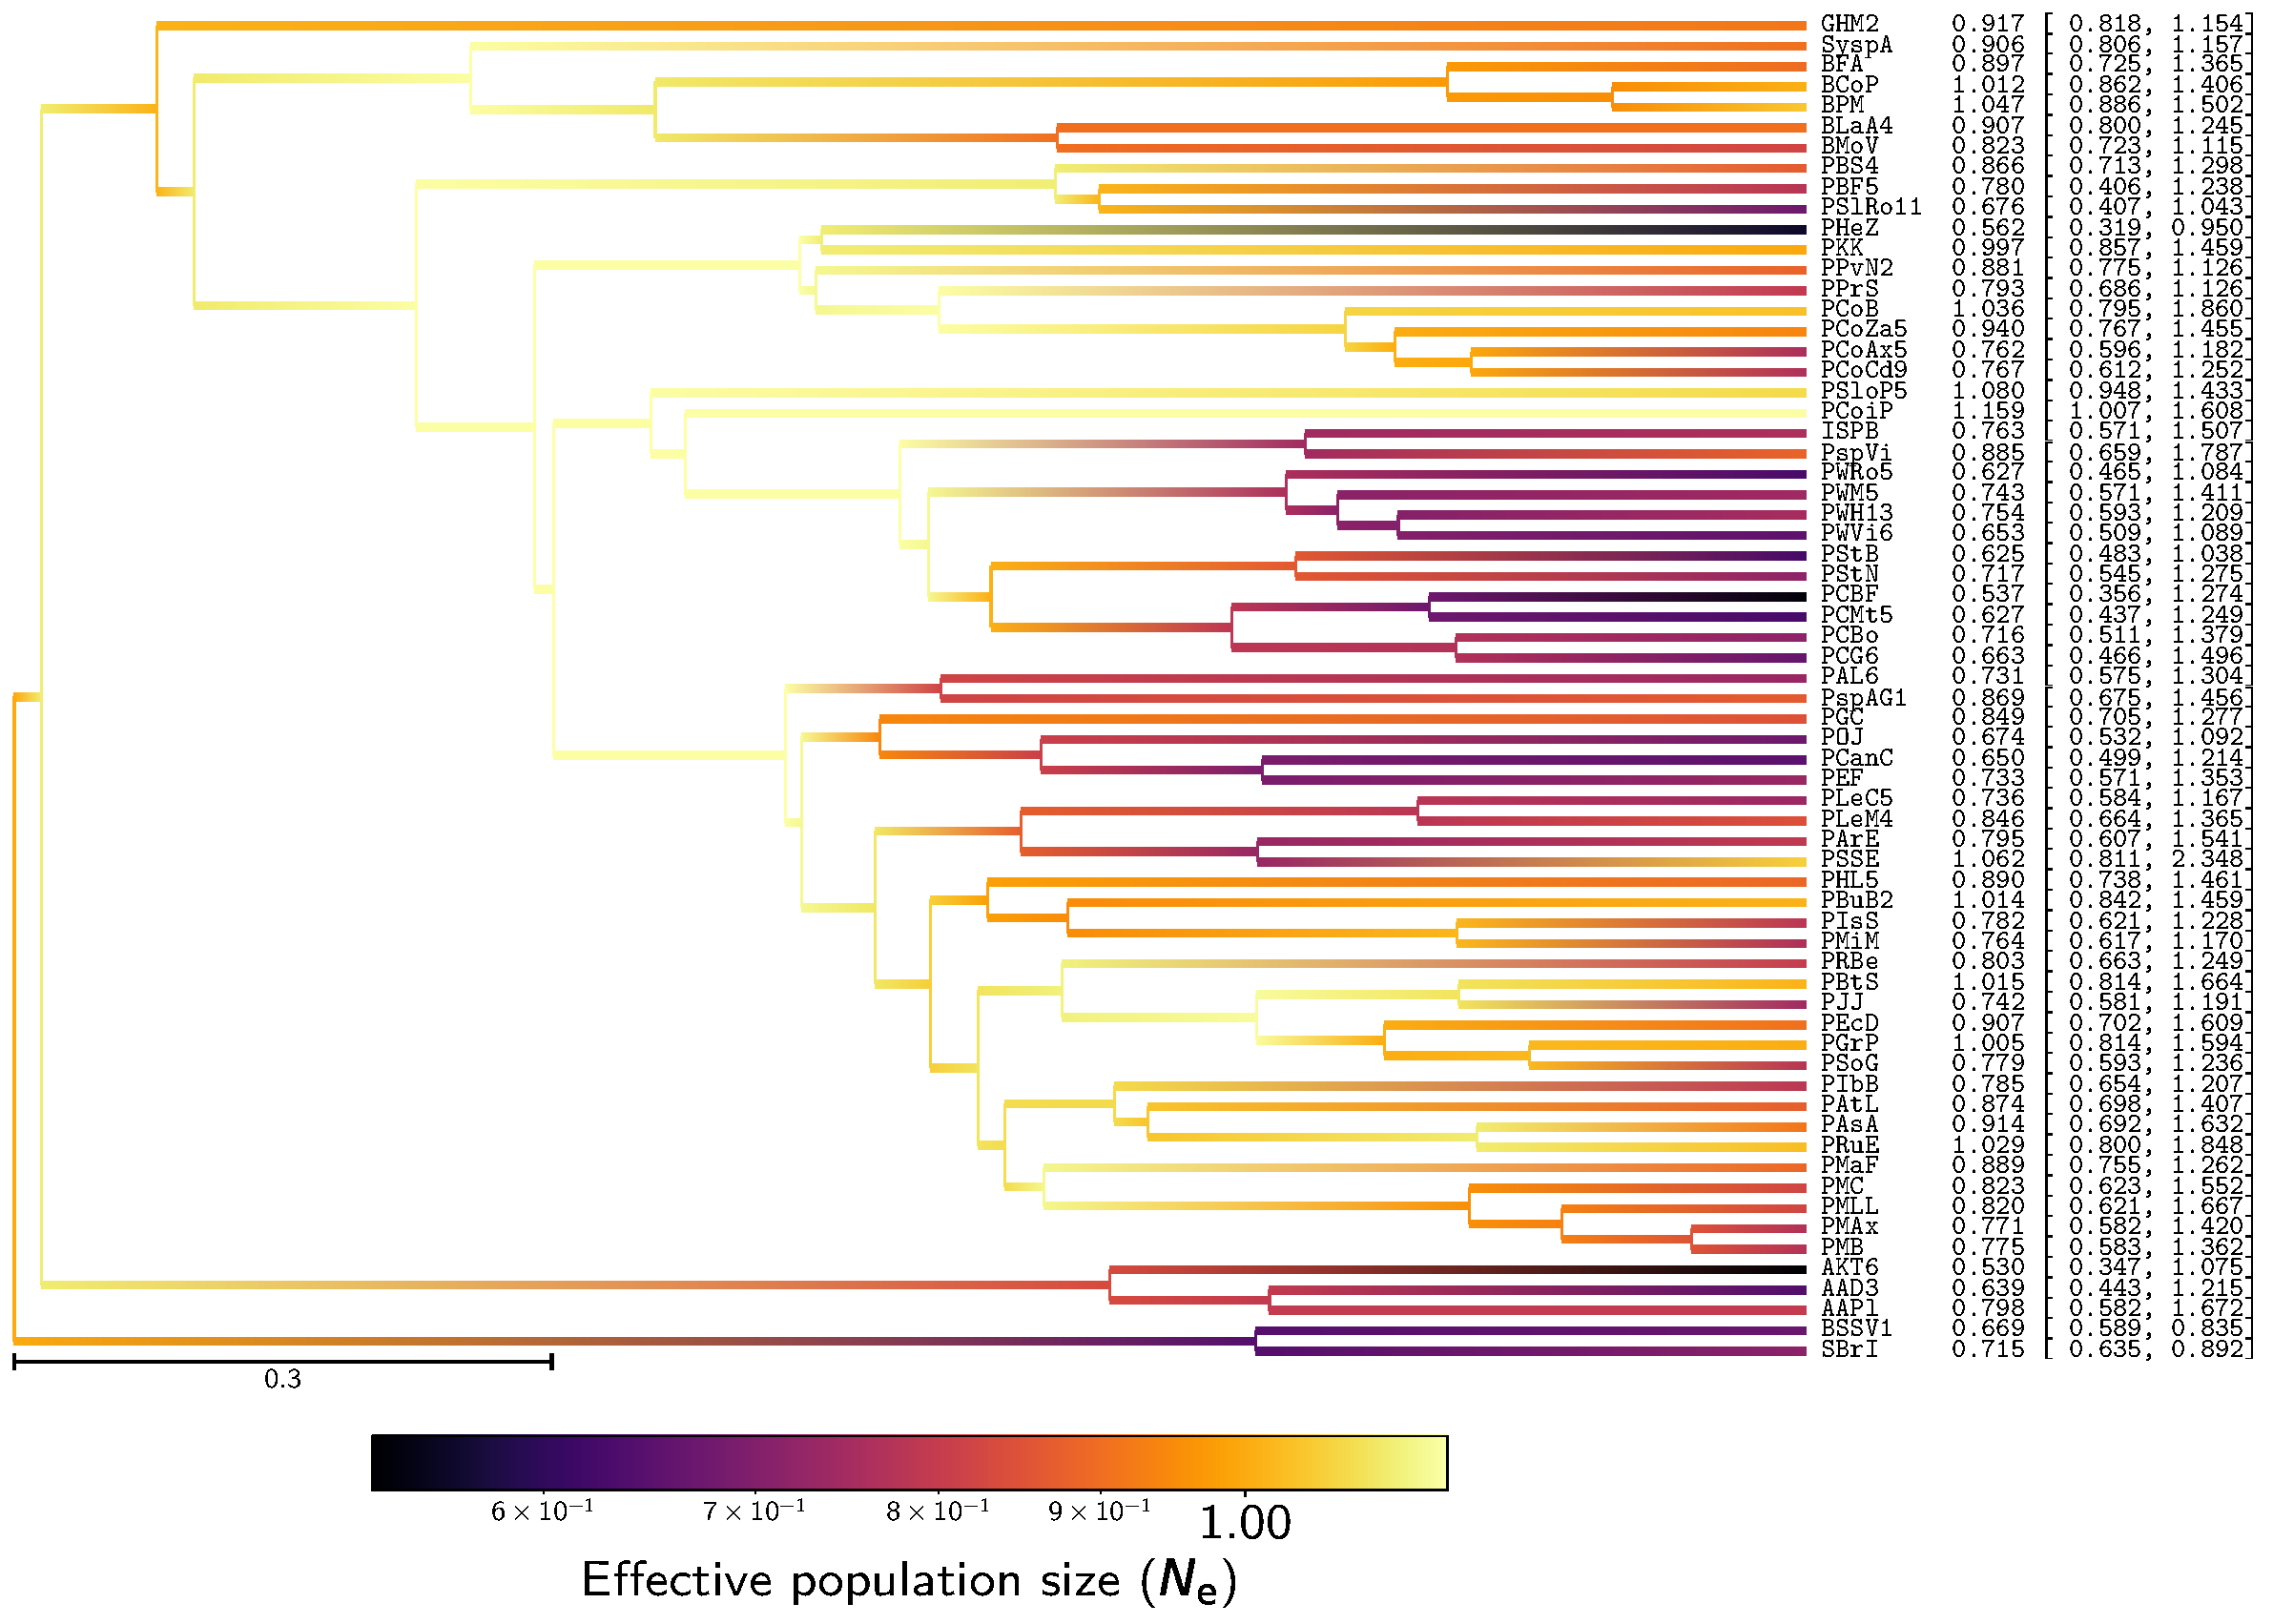
\includegraphics[width=\linewidth, page=1]{isopods/12CDS_SiteMutSelBranchNe_R1_LogPopulationSize}
    \caption[$\Ne$ estimation in isopods]{Effective population size ($\Ne$) estimation in isopods}
\end{figure}

\begin{figure}[H]
    \centering
    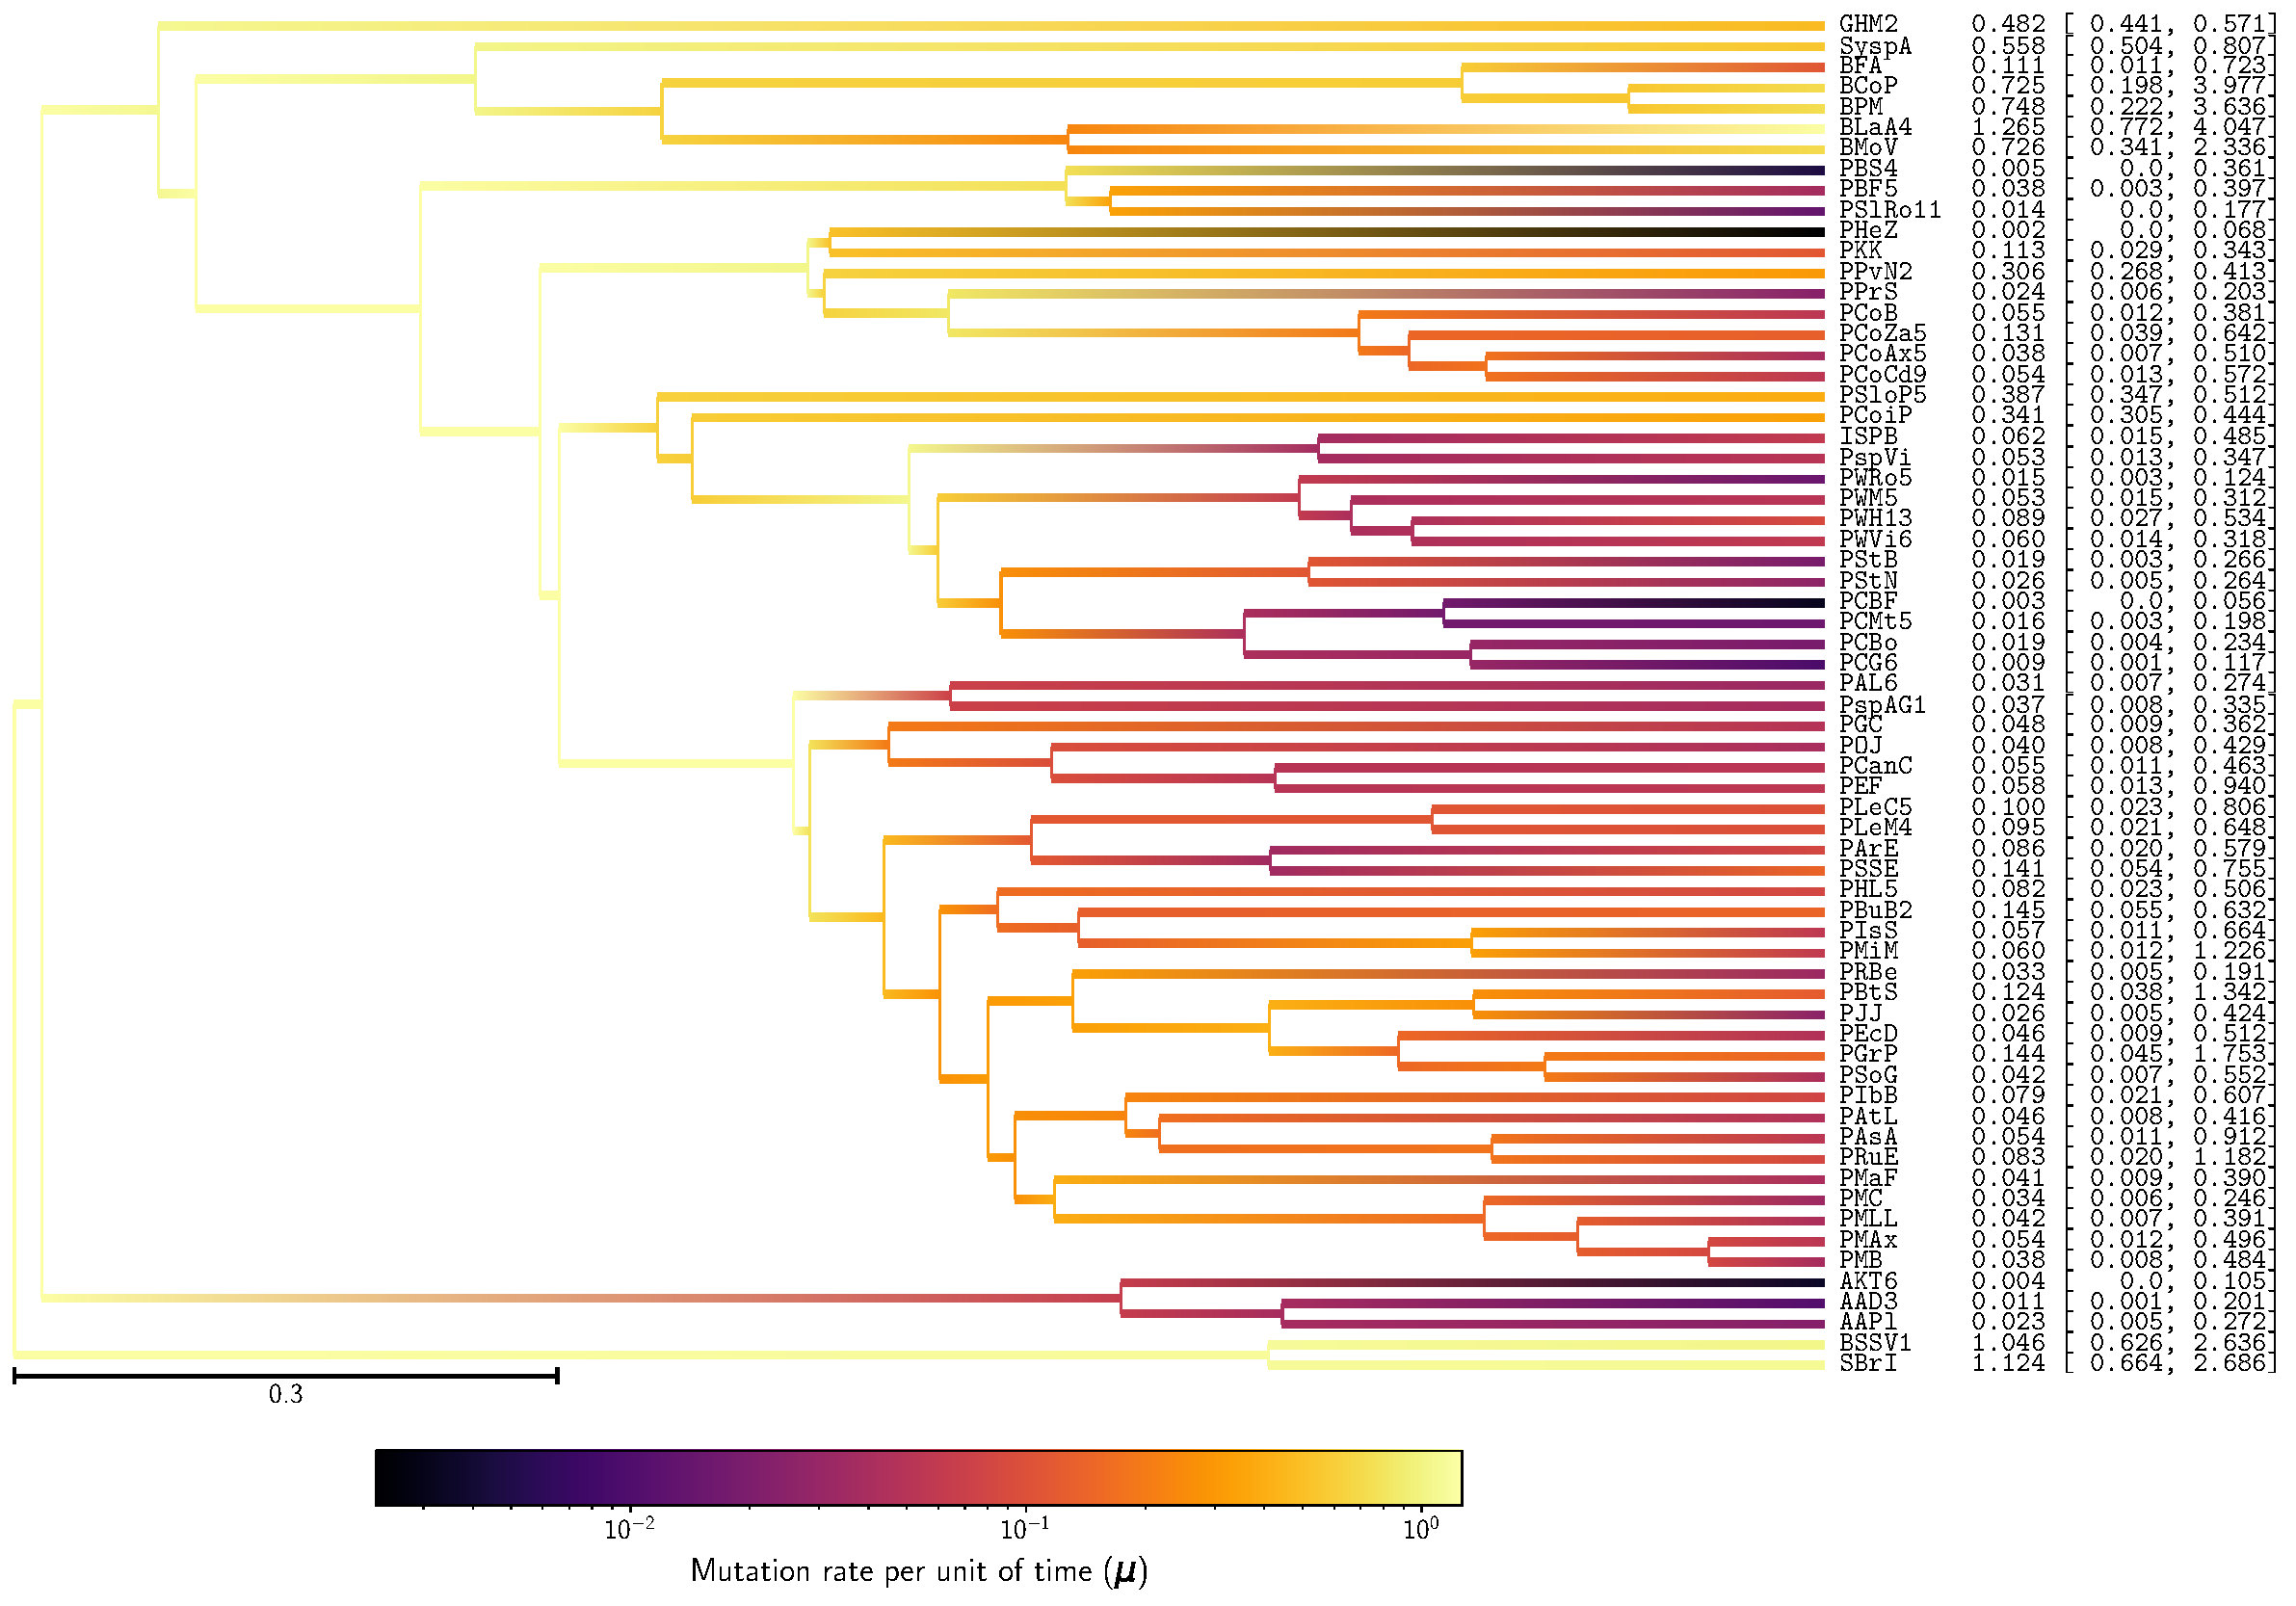
\includegraphics[width=\linewidth, page=1]{isopods/12CDS_SiteMutSelBranchNe_R1_LogMutationRatePerTime}
    \caption[Mutation rate estimation in isopods]{Mutation rate ($\mu$) estimation in isopods}
\end{figure}

\subsection{Repeatability of experiments}
Obtained with the inference model of site selection for amino acid, and branch fluctuation of $\Ne$.

\begin{figure}[H]
    \centering
    \begin{minipage}{0.32\linewidth}
        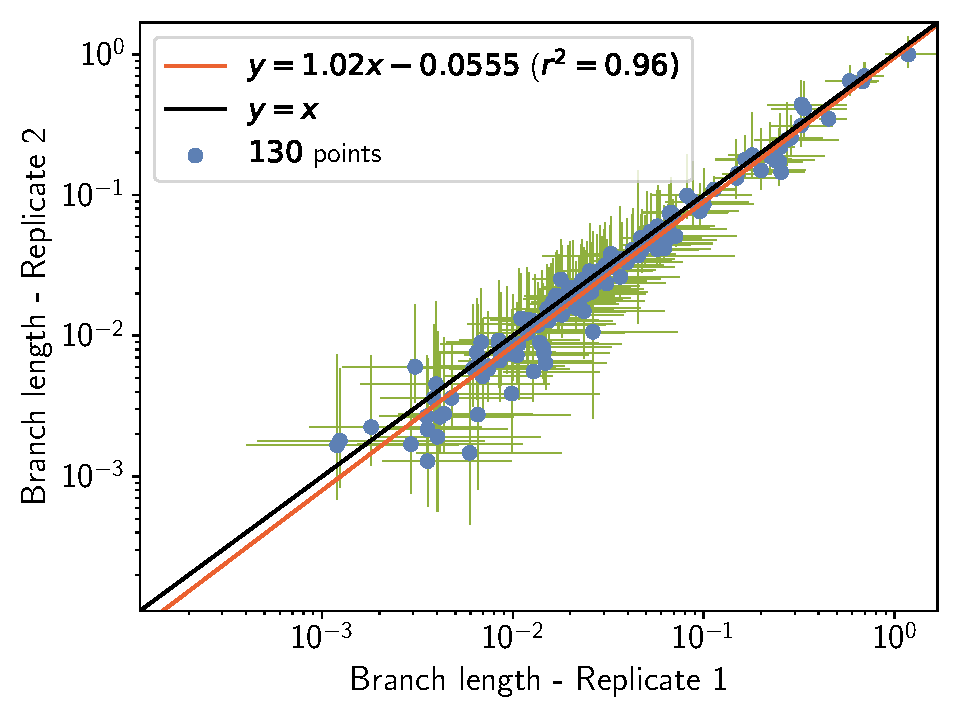
\includegraphics[width=\linewidth, page=1]{isopods/12CDS_SiteMutSelBranchNe_Rep-1-2_Log10BranchLength}
    \end{minipage} \hfill
    \begin{minipage}{0.32\linewidth}
        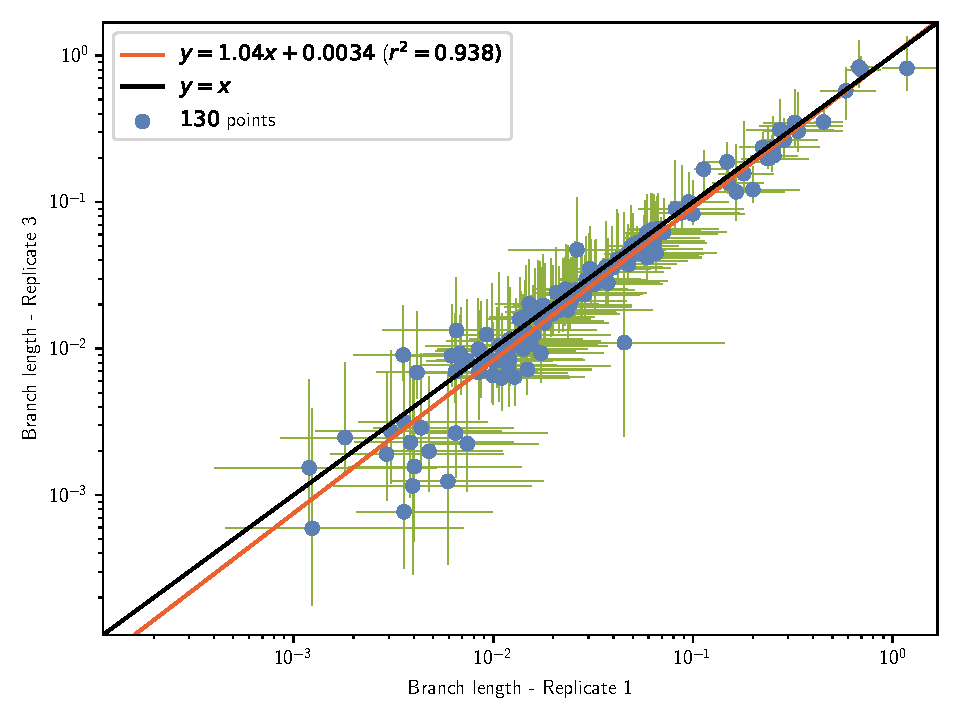
\includegraphics[width=\linewidth, page=1]{isopods/12CDS_SiteMutSelBranchNe_Rep-1-3_Log10BranchLength}
    \end{minipage} \hfill
    \begin{minipage}{0.32\linewidth}
        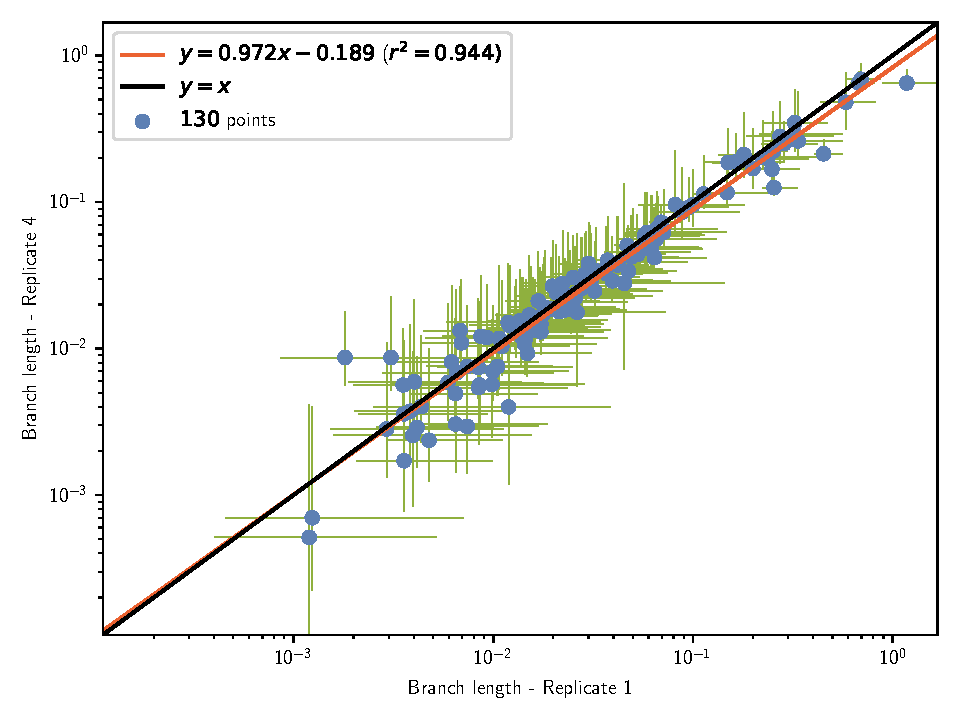
\includegraphics[width=\linewidth, page=1]{isopods/12CDS_SiteMutSelBranchNe_Rep-1-4_Log10BranchLength}
    \end{minipage}
    \begin{minipage}{0.32\linewidth}
        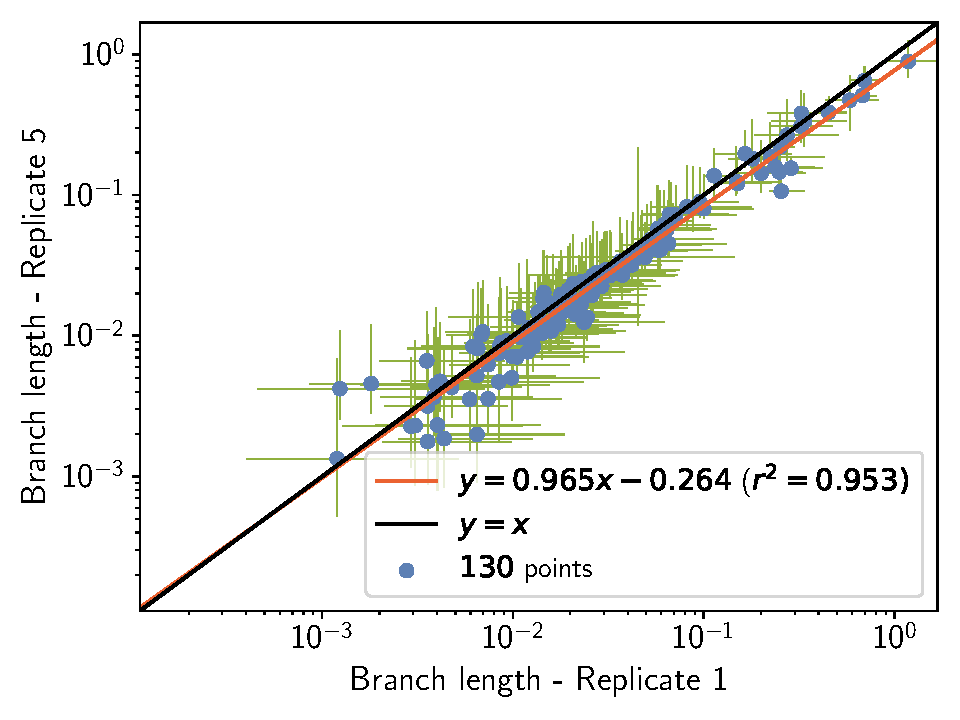
\includegraphics[width=\linewidth, page=1]{isopods/12CDS_SiteMutSelBranchNe_Rep-1-5_Log10BranchLength}
    \end{minipage}
    \begin{minipage}{0.32\linewidth}
        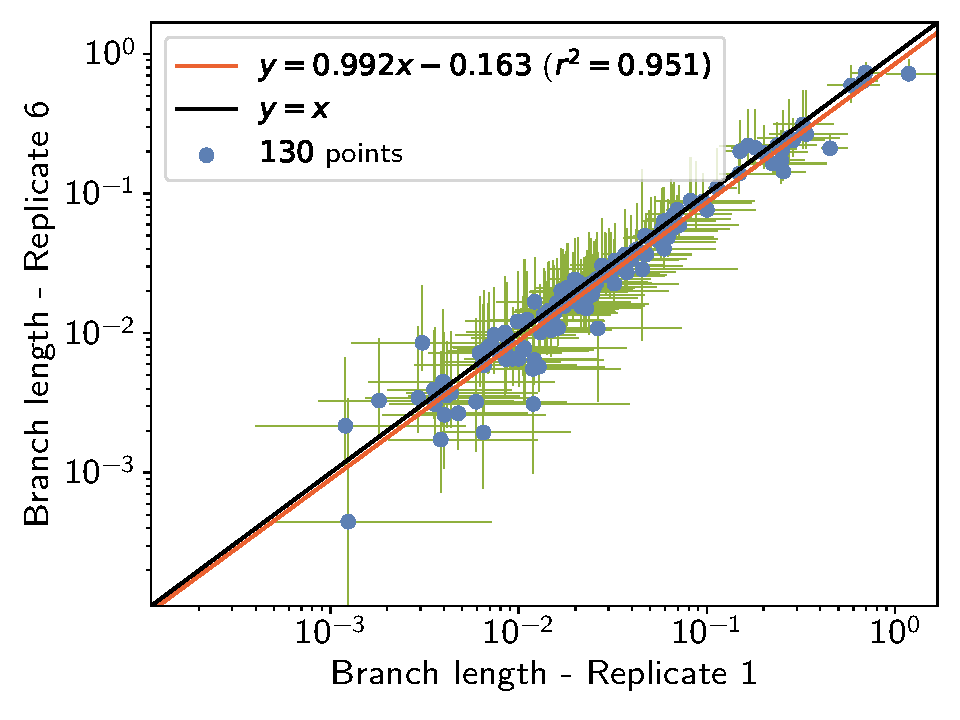
\includegraphics[width=\linewidth, page=1]{isopods/12CDS_SiteMutSelBranchNe_Rep-1-6_Log10BranchLength}
    \end{minipage}
    \caption[Repeatability of branch length estimation in isopods]{Repeatability of branch length ($\branchlength$) estimation in isopods}
\end{figure}

\begin{figure}[H]
    \centering
    \begin{minipage}{0.32\linewidth}
        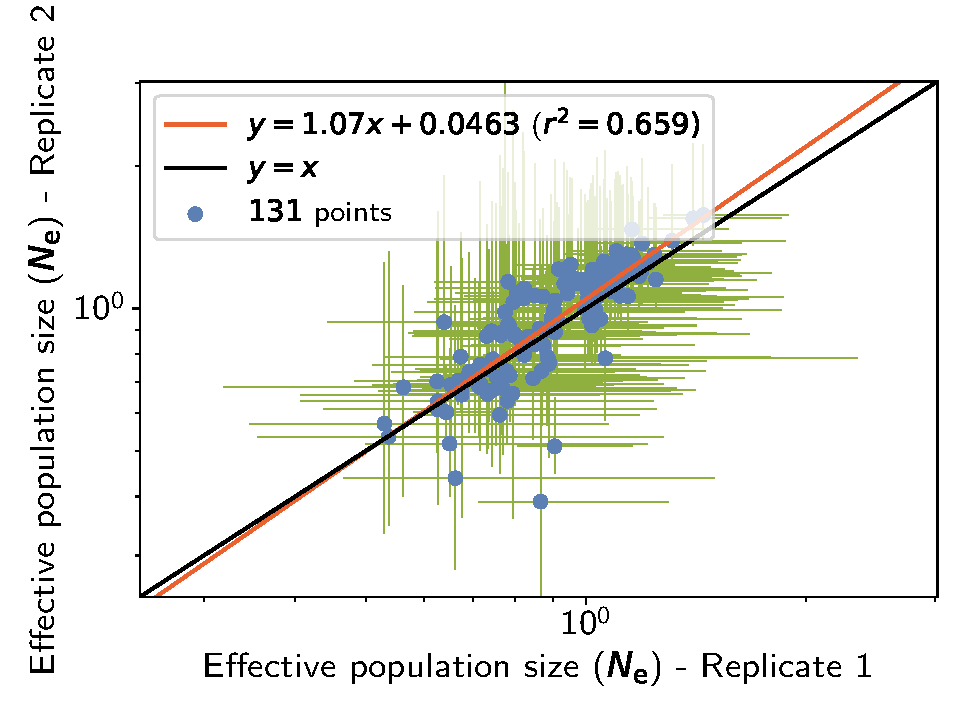
\includegraphics[width=\linewidth, page=1]{isopods/12CDS_SiteMutSelBranchNe_Rep-1-2_LogPopulationSize}
    \end{minipage} \hfill
    \begin{minipage}{0.32\linewidth}
        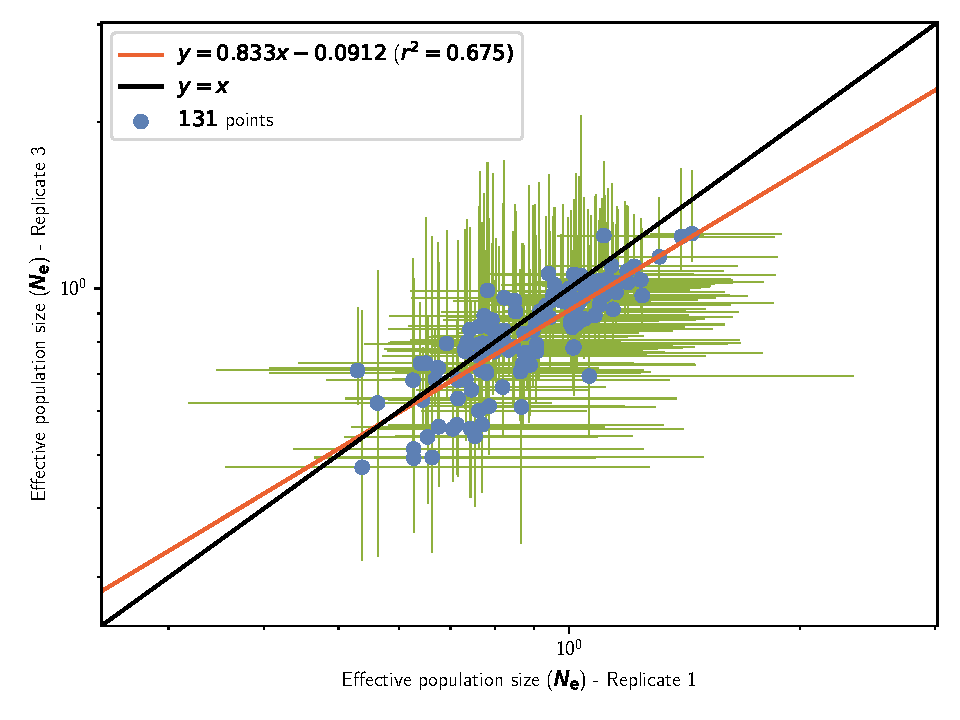
\includegraphics[width=\linewidth, page=1]{isopods/12CDS_SiteMutSelBranchNe_Rep-1-3_LogPopulationSize}
    \end{minipage} \hfill
    \begin{minipage}{0.32\linewidth}
        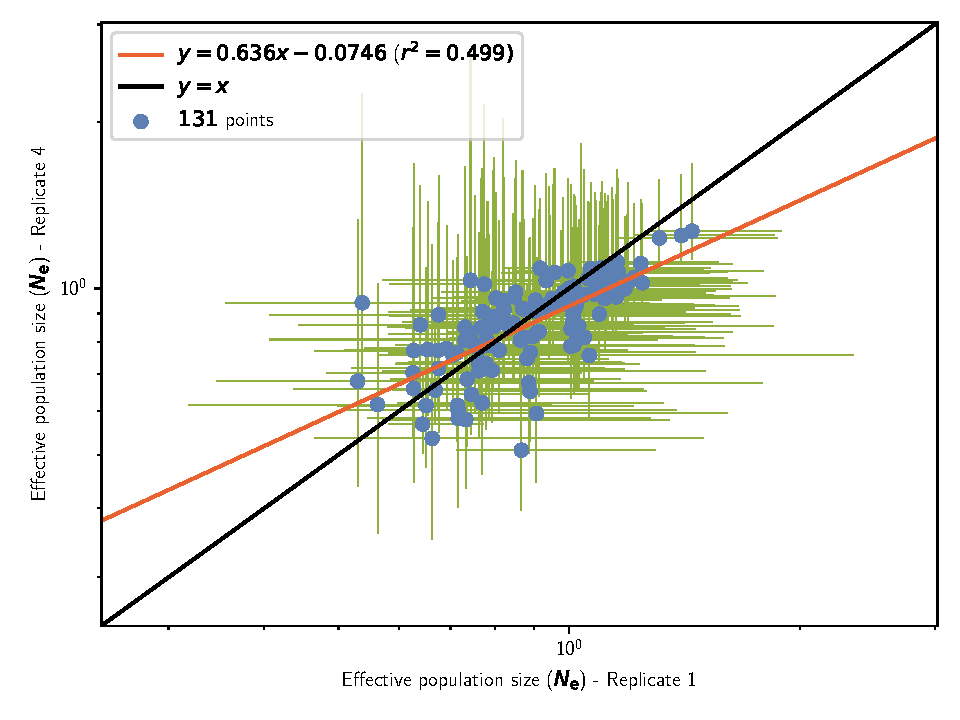
\includegraphics[width=\linewidth, page=1]{isopods/12CDS_SiteMutSelBranchNe_Rep-1-4_LogPopulationSize}
    \end{minipage}
    \begin{minipage}{0.32\linewidth}
        \includegraphics[width=\linewidth, page=1]{isopods/12CDS_SiteMutSelBranchNe_Rep-1-5_LogPopulationSize}
    \end{minipage}
    \begin{minipage}{0.32\linewidth}
        \includegraphics[width=\linewidth, page=1]{isopods/12CDS_SiteMutSelBranchNe_Rep-1-6_LogPopulationSize}
    \end{minipage}
    \caption[Repeatability of $\Ne$ estimation in isopods]{Repeatability of {effective population size} ($\Ne$) estimation in isopods}
\end{figure}

\begin{figure}[H]
    \centering
    \begin{minipage}{0.32\linewidth}
        \includegraphics[width=\linewidth, page=1]{isopods/12CDS_SiteMutSelBranchNe_Rep-1-2_LogMutationRatePerTime}
    \end{minipage} \hfill
    \begin{minipage}{0.32\linewidth}
        \includegraphics[width=\linewidth, page=1]{isopods/12CDS_SiteMutSelBranchNe_Rep-1-3_LogMutationRatePerTime}
    \end{minipage} \hfill
    \begin{minipage}{0.32\linewidth}
        \includegraphics[width=\linewidth, page=1]{isopods/12CDS_SiteMutSelBranchNe_Rep-1-4_LogMutationRatePerTime}
    \end{minipage}
    \begin{minipage}{0.32\linewidth}
        \includegraphics[width=\linewidth, page=1]{isopods/12CDS_SiteMutSelBranchNe_Rep-1-5_LogMutationRatePerTime}
    \end{minipage}
    \begin{minipage}{0.32\linewidth}
        \includegraphics[width=\linewidth, page=1]{isopods/12CDS_SiteMutSelBranchNe_Rep-1-6_LogMutationRatePerTime}
    \end{minipage}
    \caption[Repeatability of $\mu$ estimation in isopods]{Repeatability of mutation rate ($\mu$) estimation in isopods}
\end{figure}

\begin{figure}[H]
    \centering
    \begin{minipage}{0.32\linewidth}
        \includegraphics[width=\linewidth, page=1]{isopods/12CDS_SiteMutSelBranchNe_Rep-1-2_BranchTime}
    \end{minipage} \hfill
    \begin{minipage}{0.32\linewidth}
        \includegraphics[width=\linewidth, page=1]{isopods/12CDS_SiteMutSelBranchNe_Rep-1-3_BranchTime}
    \end{minipage} \hfill
    \begin{minipage}{0.32\linewidth}
        \includegraphics[width=\linewidth, page=1]{isopods/12CDS_SiteMutSelBranchNe_Rep-1-4_BranchTime}
    \end{minipage}
    \begin{minipage}{0.32\linewidth}
        \includegraphics[width=\linewidth, page=1]{isopods/12CDS_SiteMutSelBranchNe_Rep-1-5_BranchTime}
    \end{minipage}
    \begin{minipage}{0.32\linewidth}
        \includegraphics[width=\linewidth, page=1]{isopods/12CDS_SiteMutSelBranchNe_Rep-1-6_BranchTime}
    \end{minipage}
    \caption[Repeatability of branch time estimation in isopods]{Repeatability of branch time ($\Delta T$) estimation in isopods}
\end{figure}

\subsection{Statistical test}
Obtained with the inference model of site selection for amino acid, and branch fluctuation of $\Ne$.

\begin{figure}[H]
    \centering
    \includegraphics[width=\linewidth, page=1]{isopods/12CDS_SiteMutSelBranchNe_Rep_LogPopulationSize_eco}
    \caption[$\Ne$ as a function of habitat in isopods]{$\Ne$ as a function of habitat in isopods.}
\end{figure}
\begin{verbatim}
Analysis of Variance Table

Response: PopulationSize
Df Sum Sq Mean Sq F value Pr(>F) 
Habitat 1 2.4899 2.48991 83.2450 < 2.2e-16 ***
Replicate 5 0.6446 0.12892 4.3102 0.0007908 ***
Residuals 389 11.6352 0.02991 
---
Signif. codes: 0 ‘***’ 0.001 ‘**’ 0.01 ‘*’ 0.05 ‘.’ 0.1 ‘ ’ 1
\end{verbatim}
\begin{figure}[H]
    \centering
    \includegraphics[width=\linewidth, page=1]{isopods/12CDS_SiteMutSelBranchNe_Rep_LogPopulationSize_pig}
    \caption[$\Ne$ as a function of pigmentation in isopods]{$\Ne$ as a function of pigmentation in isopods}
\end{figure}
\begin{verbatim}
Analysis of Variance Table

Response: PopulationSize
Df Sum Sq Mean Sq F value Pr(>F) 
Pigmentation 2 2.8413 1.42067 48.850 < 2.2e-16 ***
Replicate 5 0.6446 0.12892 4.433 0.0006135 ***
Residuals 388 11.2838 0.02908 
---
Signif. codes: 0 ‘***’ 0.001 ‘**’ 0.01 ‘*’ 0.05 ‘.’ 0.1 ‘ ’ 1
\end{verbatim}
\begin{figure}[H]
    \centering
    \includegraphics[width=\linewidth, page=1]{isopods/12CDS_SiteMutSelBranchNe_Rep_LogPopulationSize_eye}
    \caption[$\Ne$ as a function of ocular structure in isopods]{$\Ne$ as a function of ocular structure in isopods}
\end{figure}
\begin{verbatim}
Analysis of Variance Table

Response: PopulationSize
Df Sum Sq Mean Sq F value Pr(>F) 
Ocular.structure 2 2.8463 1.42314 48.9571 < 2.2e-16 ***
Replicate 5 0.6446 0.12892 4.4349 0.000611 ***
Residuals 388 11.2789 0.02907 
---
Signif. codes: 0 ‘***’ 0.001 ‘**’ 0.01 ‘*’ 0.05 ‘.’ 0.1 ‘ ’ 1
\end{verbatim}
\begin{figure}[H]
    \centering
    \begin{minipage}{0.32\linewidth}
        \includegraphics[width=\linewidth, page=1]{isopods/12CDS_SiteMutSelBranchNe_Rep_LogPopulationSize_eco_merged}
    \end{minipage} \hfill
    \begin{minipage}{0.32\linewidth}
        \includegraphics[width=\linewidth, page=1]{isopods/12CDS_SiteMutSelBranchNe_Rep_LogPopulationSize_pig_merged}
    \end{minipage} \hfill
    \begin{minipage}{0.32\linewidth}
        \includegraphics[width=\linewidth, page=1]{isopods/12CDS_SiteMutSelBranchNe_Rep_LogPopulationSize_eye_merged}
    \end{minipage}
    \caption[$\Ne$ as a function of traits in isopods]{$\Ne$ as a function of traits in isopods}
\end{figure}


\section{Empirical data in Primates}
\label{sec:empirical-data-in-primates}

\subsection{Chain convergence}
Obtained with the inference model of site selection for amino acid, and branch fluctuation of $\Ne$.

\begin{figure}[H]
    \centering
    \begin{minipage}{0.49\linewidth}
        \includegraphics[width=\linewidth, page=1]{primates/SiteMutSelBranchNe_ProfileCorrelation.png}
    \end{minipage} \hfill
    \begin{minipage}{0.49\linewidth}
        \includegraphics[width=\linewidth, page=1]{primates/SiteMutSelBranchNe_LogPopulationSizeCorrelation}
    \end{minipage}
    \caption[Chain convergence of site profiles and branche $\Ne$]{
    Chain convergence of site amino-acid preferences (left panel) and branch $\Ne$ (right panel).}
\end{figure}

\subsection{Traits estimation (chain~1)}
Obtained with the inference model of site selection for amino acid, and branch fluctuation of $\Ne$.

\begin{table}[H]
    \centering
\noindent\adjustbox{max width=\textwidth}{%
\begin{tabu}{|c||c|c|c|c|c|c|c|c|}
\hline
\textbf{Correlation ($\bm{\rho}$)} & $\bm{N_{\text{e}}}$ & $\bm{\mu}$ & \textbf{maturity} & \textbf{mass} & \textbf{longevity} & $\bm{\pi_{S}}$ & $\bm{\pi_{N}/\pi_{S}}$ & \textbf{generation time}\\
\hhline{|=#=|=|=|=|=|=|=|=|}
$\bm{N_{\text{e}}}$ & - & $-0.433^{**}$ & $0.155$ & $0.166$ & $0.157$ & $-0.133$ & $0.104$ & $0.16$\\\hline
$\bm{\mu}$ & - & - & $-0.792^{**}$ & $-0.791^{**}$ & $-0.773^{**}$ & $0.62^{**}$ & $-0.59$ & $-0.78^{**}$\\\hline
\textbf{maturity} & - & - & - & $0.986^{**}$ & $0.985^{**}$ & $-0.8^{**}$ & $0.746$ & $0.991^{**}$\\\hline
\textbf{mass} & - & - & - & - & $0.977^{**}$ & $-0.737^{**}$ & $0.695$ & $0.981^{**}$\\\hline
\textbf{longevity} & - & - & - & - & - & $-0.819^{**}$ & $0.752$ & $0.999^{**}$\\\hline
$\bm{\pi_{S}}$ & - & - & - & - & - & - & $-0.86^{**}$ & $-0.816^{**}$\\\hline
$\bm{\pi_{N}/\pi_{S}}$ & - & - & - & - & - & - & - & $0.752$\\\hline
\textbf{generation time} & - & - & - & - & - & - & - & -\\\hline
\end{tabu}}

    \caption[Correlation coefficient matrix in primates ($\Ne$)]{
    Correlation coefficient between effective population size~($\Ne$), mutation rate per site per unit of time~($\mu$), and life-history traits (maximum longevity, adult weight and female maturity) were computed in placental mammals.
    Asterisks indicate strength of support ($\smash{^{*}} pp > 0.95$, $\smash{^{**}} pp > 0.975$).}
\end{table}

\begin{table}[H]
    \centering
\noindent\adjustbox{max width=\textwidth}{%
\begin{tabu}{|c||c|c|c|c|c|c|c|c|}
\hline
\textbf{Covariance ($\bm{\Sigma}$)} & $\bm{N_{\text{e}}}$ & $\bm{\mu}$ & \textbf{maturity} & \textbf{mass} & \textbf{longevity} & $\bm{\pi_{S}}$ & $\bm{\pi_{N}/\pi_{S}}$ & \textbf{generation time}\\
\hhline{|=#=|=|=|=|=|=|=|=|}
$\bm{N_{\text{e}}}$ & $1.08^{**}$ & $-1.39^{**}$ & $0.66$ & $1.18$ & $0.414$ & $-0.251$ & $0.0898$ & $0.452$\\\hline
$\bm{\mu}$ & - & $9.86^{**}$ & $-10.1^{**}$ & $-17.5^{**}$ & $-6.44^{**}$ & $3.42^{**}$ & $-1.28$ & $-6.96^{**}$\\\hline
\textbf{maturity} & - & - & $16.9^{**}$ & $28.4^{**}$ & $10.6^{**}$ & $-5.39^{**}$ & $1.9$ & $11.5^{**}$\\\hline
\textbf{mass} & - & - & - & $49.8^{**}$ & $18.1^{**}$ & $-8.89^{**}$ & $3.29$ & $19.5^{**}$\\\hline
\textbf{longevity} & - & - & - & - & $6.99^{**}$ & $-3.75^{**}$ & $1.31$ & $7.47^{**}$\\\hline
$\bm{\pi_{S}}$ & - & - & - & - & - & $3.26^{**}$ & $-0.986^{**}$ & $-3.96^{**}$\\\hline
$\bm{\pi_{N}/\pi_{S}}$ & - & - & - & - & - & - & $0.419^{**}$ & $1.39$\\\hline
\textbf{generation time} & - & - & - & - & - & - & - & $8.02^{**}$\\\hline
\end{tabu}}

    \caption[Covariance matrix in primates ($\Ne$)]{
    Correlation coefficient between effective population size~($\Ne$), mutation rate per site per unit of time~($\mu$), and life-history traits (maximum longevity, adult weight and female maturity) were computed in placental mammals.
    Asterisks indicate strength of support ($\smash{^{*}} pp > 0.95$, $\smash{^{**}} pp > 0.975$).}
\end{table}

\begin{table}[H]
    \centering
\noindent\adjustbox{max width=\textwidth}{%
\begin{tabu}{|c||c|c|c|c|c|c|c|c|}
\hline
\textbf{Partial coefficient} & $\bm{N_{\mathrm{e}}}$ & $\bm{\mu}$ & \textbf{maturity} & \textbf{mass} & \textbf{longevity} & $\bm{\pi_{S}}$ & $\bm{\pi_{N}/\pi_{S}}$ & \textbf{generation time}\\
\hhline{|=#=|=|=|=|=|=|=|=|}
$\bm{N_{\mathrm{e}}}$ & - & $-0.411$ & $-0.0622$ & $0.0184$ & $-0.0436$ & $-0.0482$ & $-0.00476$ & $0.0333$\\\hline
$\bm{\mu}$ & - & - & $0.0548$ & $-0.101$ & $0.146$ & $-0.0134$ & $-0.102$ & $-0.124$\\\hline
\textbf{maturity} & - & - & - & $0.292$ & $-0.793^{**}$ & $-0.167$ & $0.0547$ & $0.824^{**}$\\\hline
\textbf{mass} & - & - & - & - & $-0.0589$ & $0.43$ & $-0.195$ & $0.101$\\\hline
\textbf{longevity} & - & - & - & - & - & $-0.159$ & $-0.148$ & $0.991^{**}$\\\hline
$\bm{\pi_{S}}$ & - & - & - & - & - & - & $-0.573^{**}$ & $0.11$\\\hline
$\bm{\pi_{N}/\pi_{S}}$ & - & - & - & - & - & - & - & $0.144$\\\hline
\textbf{generation time} & - & - & - & - & - & - & - & -\\\hline
\end{tabu}}

    \caption[Partial correlation coefficient matrix in primates ($\Ne$)]{
    Partial correlation coefficient between Neffective population size~($\Ne$), mutation rate per site per unit of time~($\mu$), and life-history traits (maximum longevity, adult weight and female maturity) were computed in placental mammals.
    Asterisks indicate strength of support ($\smash{^{*}} pp > 0.95$, $\smash{^{**}} pp > 0.975$).}
\end{table}

\begin{figure}[H]
    \centering
    \includegraphics[width=\linewidth, page=1]{primates/SiteMutSelBranchNe_LogPopulationSize}
    \caption[$\Ne$ estimation in primates]{Effective population size ($\Ne$) estimation in primates}
\end{figure}

\begin{figure}[H]
    \centering
    \includegraphics[width=\linewidth, page=1]{primates/SiteMutSelBranchNe_LogMutationRatePerTime}
    \caption[Mutation rate estimation in primates]{Mutation rate ($\mu$) estimation in primates}
\end{figure}

\begin{figure}[H]
    \centering
    \includegraphics[width=\linewidth, page=1]{primates/SiteMutSelBranchNe_Logmaturity}
    \caption[Female maturity estimation in primates]{Female maturity estimation in primates}
\end{figure}

\begin{figure}[H]
    \centering
    \includegraphics[width=\linewidth, page=1]{primates/SiteMutSelBranchNe_Logmass}
    \caption[Mass estimation in primates]{Mass estimation in primates}
\end{figure}

\begin{figure}[H]
    \centering
    \includegraphics[width=\linewidth, page=1]{primates/SiteMutSelBranchNe_Loglongevity}
    \caption[Longevity estimation in primates]{Longevity estimation in primates}
\end{figure}

\begin{figure}[H]
    \centering
    \includegraphics[width=\linewidth, page=1]{primates/SiteMutSelBranchNe_LogpiS}
    \caption[$\pi_{S}$ estimation in primates]{$\pi_{S}$ estimation in primates}
\end{figure}

\begin{figure}[H]
    \centering
    \includegraphics[width=\linewidth, page=1]{primates/SiteMutSelBranchNe_LogpiNpiS}
    \caption[$\pi_{N} / \pi_{S}$ estimation in primates]{$\pi_{N} / \pi_{S}$ estimation in primates}
\end{figure}

\begin{figure}[H]
    \centering
    \includegraphics[width=\linewidth, page=1]{primates/SiteMutSelBranchNe_Loggeneration_time}
    \caption[Generation time estimation in primates]{Generation time estimation in primates}
\end{figure}

\subsection{Amino-acid preferences entropy}

\begin{table}[H]
    \centering
    \noindent\adjustbox{max width=\textwidth}{%
    \begin{tabu}{|c|c|c|}
        \hline
        \textbf{Experiment} & $\langle \entropy \rangle$ (\textbf{branch} $\Ne$) & $\langle \entropy \rangle$ (\textbf{constant} $\Ne$) \\ \hline
        \hline
        Primates, chain~1 & $1.41 \pm 0.10$ & $1.49 \pm 0.08$\\ \hline
        Primates, chain 2 & $1.40 \pm 0.10$ & $1.48 \pm 0.08$\\ \hline
    \end{tabu}}
    \caption[Amino-acid entropy in primates]{Estimated amino acids entropy in primates.
    Obtained with the inference model of site selection for amino acid, and branch fluctuation of $\Ne$ (left column), or under the assumption of constant $\Ne$ (right column)}
\end{table}

\subsection{Traits estimation with branch \texorpdfstring{$\omega$}{ω} (chain~1)}
Obtained with the model of branch fluctuation of $\dnds$ (without site selection for amino acid).

\begin{figure}[H]
    \centering
    \includegraphics[width=\linewidth, page=1]{primates/BranchOmega_LogOmega}
    \caption[$\dnds$ estimation in primates]{{Non-synonymous substitution} rate ($\dnds$) estimation in primates}
\end{figure}

\begin{figure}[H]
    \centering
    \includegraphics[width=\linewidth, page=1]{primates/BranchOmega_LogMutationRatePerTime}
    \caption[$\mu$ estimation in primates]{Mutation rate ($\mu$) estimation in primates}
\end{figure}

\begin{table}[H]
    \centering
\noindent\adjustbox{max width=\textwidth}{%
\begin{tabu}{|c||c|c|c|c|c|c|c|c|}
\hline
\textbf{Correlation ($\bm{\rho}$)} & $\bm{\omega}$ & $\bm{\mu}$ & \textbf{maturity} & \textbf{mass} & \textbf{longevity} & $\bm{\pi_{S}}$ & $\bm{\pi_{N}/\pi_{S}}$ & \textbf{generation time}\\
\hhline{|=#=|=|=|=|=|=|=|=|}
$\bm{\omega}$ & - & $0.294$ & $0.000316$ & $0.0361$ & $0.0155$ & $-0.197$ & $0.145$ & $0.0111$\\\hline
$\bm{\mu}$ & - & - & $-0.804^{**}$ & $-0.798^{**}$ & $-0.817^{**}$ & $-0.0201$ & $0.031$ & $-0.823^{**}$\\\hline
\textbf{maturity} & - & - & - & $0.952^{**}$ & $0.957^{**}$ & $-0.166$ & $0.162$ & $0.97^{**}$\\\hline
\textbf{mass} & - & - & - & - & $0.933^{**}$ & $-0.0437$ & $0.0427$ & $0.943^{**}$\\\hline
\textbf{longevity} & - & - & - & - & - & $-0.223$ & $0.165$ & $0.999^{**}$\\\hline
$\bm{\pi_{S}}$ & - & - & - & - & - & - & $-0.664$ & $-0.212$\\\hline
$\bm{\pi_{N}/\pi_{S}}$ & - & - & - & - & - & - & - & $0.162$\\\hline
\textbf{generation time} & - & - & - & - & - & - & - & -\\\hline
\end{tabu}}

    \caption[Correlation coefficient matrix in primates ($\dnds$)]{
    Correlation coefficient between non-synonymous substitution rate~($\dnds$), mutation rate per site per unit of time~($\mu$), and life-history traits (maximum longevity, adult weight and female maturity) were computed in placental mammals.
    Asterisks indicate strength of support ($\smash{^{*}} pp > 0.95$, $\smash{^{**}} pp > 0.975$).}
\end{table}

\begin{table}[H]
    \centering
\noindent\adjustbox{max width=\textwidth}{%
\begin{tabu}{|c||c|c|c|c|c|c|c|c|}
\hline
\textbf{Covariance ($\bm{\Sigma}$)} & $\bm{\omega}$ & $\bm{\mu}$ & \textbf{maturity} & \textbf{mass} & \textbf{longevity} & $\bm{\pi_{S}}$ & $\bm{\pi_{N}/\pi_{S}}$ & \textbf{generation time}\\
\hhline{|=#=|=|=|=|=|=|=|=|}
$\bm{\omega}$ & $0.0674^{**}$ & $0.231$ & $-0.0106$ & $0.0149$ & $-0.00138$ & $-0.0435$ & $0.0101$ & $-0.00314$\\\hline
$\bm{\mu}$ & - & $8.71^{**}$ & $-4.8^{**}$ & $-9.22^{**}$ & $-3.97^{**}$ & $0.188$ & $0.0483$ & $-4.08^{**}$\\\hline
\textbf{maturity} & - & - & $4.95^{**}$ & $8.37^{**}$ & $3.29^{**}$ & $-1.01$ & $0.000924$ & $3.53^{**}$\\\hline
\textbf{mass} & - & - & - & $16.3^{**}$ & $6.14^{**}$ & $-0.932$ & $-0.0741$ & $6.45^{**}$\\\hline
\textbf{longevity} & - & - & - & - & $2.76^{**}$ & $-0.577$ & $0.0919$ & $2.82^{**}$\\\hline
$\bm{\pi_{S}}$ & - & - & - & - & - & $1.3^{**}$ & $-0.148$ & $-0.637$\\\hline
$\bm{\pi_{N}/\pi_{S}}$ & - & - & - & - & - & - & $0.182^{**}$ & $0.0775$\\\hline
\textbf{generation time} & - & - & - & - & - & - & - & $2.92^{**}$\\\hline
\end{tabu}}

    \caption[Covariance matrix in primates ($\dnds$)]{
    Correlation coefficient between non-synonymous substitution rate~($\dnds$), mutation rate per site per unit of time~($\mu$), and life-history traits (maximum longevity, adult weight and female maturity) were computed in placental mammals.
    Asterisks indicate strength of support ($\smash{^{*}} pp > 0.95$, $\smash{^{**}} pp > 0.975$).}
\end{table}

\begin{table}[H]
    \centering
\noindent\adjustbox{max width=\textwidth}{%
\begin{tabu}{|c||c|c|c|c|c|c|c|c|}
\hline
\textbf{Partial coefficient} & $\bm{\omega}$ & $\bm{\mu}$ & \textbf{maturity} & \textbf{mass} & \textbf{longevity} & $\bm{\pi_{S}}$ & $\bm{\pi_{N}/\pi_{S}}$ & \textbf{generation time}\\
\hhline{|=#=|=|=|=|=|=|=|=|}
$\bm{\omega}$ & - & $0.463$ & $-0.0461$ & $0.248$ & $-0.027$ & $-0.193$ & $-0.0681$ & $0.0319$\\\hline
$\bm{\mu}$ & - & - & $0.0649$ & $-0.000258$ & $0.0374$ & $-0.128$ & $0.115$ & $-0.075$\\\hline
\textbf{maturity} & - & - & - & $0.228$ & $-0.834^{**}$ & $-0.0991$ & $0.0491$ & $0.854^{**}$\\\hline
\textbf{mass} & - & - & - & - & $-0.038$ & $0.435$ & $-0.123$ & $0.0851$\\\hline
\textbf{longevity} & - & - & - & - & - & $-0.184$ & $-0.145$ & $0.994^{**}$\\\hline
$\bm{\pi_{S}}$ & - & - & - & - & - & - & $-0.553^{*}$ & $0.125$\\\hline
$\bm{\pi_{N}/\pi_{S}}$ & - & - & - & - & - & - & - & $0.136$\\\hline
\textbf{generation time} & - & - & - & - & - & - & - & -\\\hline
\end{tabu}}

    \caption[Partial correlation coefficient matrix in primates ($\dnds$)]{
    Partial correlation coefficient between non-synonymous substitution rate~($\dnds$), mutation rate per site per unit of time~($\mu$), and life-history traits (maximum longevity, adult weight and female maturity) were computed in placental mammals.
    Asterisks indicate strength of support ($\smash{^{*}} pp > 0.95$, $\smash{^{**}} pp > 0.975$).}
\end{table}


\section{Empirical data in drosophila}
\label{sec:empirical-data-in-drosophila}

\subsection{Traits estimation \& correlation (replicate~1, chain~1)}
Obtained with the inference model of site selection for amino acid, and branch fluctuation of $\Ne$.

\begin{table}[H]
    \centering
\noindent\adjustbox{max width=\textwidth}{%
\begin{tabu}{|c||c|c|c|}
\hline
\textbf{Correlation ($\bm{\rho}$)} & $\bm{N_{\mathrm{e}}}$ & $\bm{\mu}$ & \textbf{LogGenomeSize}\\
\hhline{|=#=|=|=|}
$\bm{N_{\mathrm{e}}}$ & - & $-0.0623$ & $-0.144$\\\hline
$\bm{\mu}$ & - & - & $0.224$\\\hline
\textbf{LogGenomeSize} & - & - & -\\\hline
\end{tabu}}

    \caption[Correlation coefficient matrix in drosophila ($\dnds$)]{
    Correlation coefficient between effective population size~($\Ne$), mutation rate per site per unit of time~($\mu$), and life-history traits (maximum longevity, adult weight and female maturity) were computed in drosophila.
    Asterisks indicate strength of support ($\smash{^{*}} pp > 0.95$, $\smash{^{**}} pp > 0.975$).}
\end{table}

\begin{table}[H]
    \centering
\noindent\adjustbox{max width=\textwidth}{%
\begin{tabu}{|c||c|c|c|c|c|}
\hline
\textbf{Covariance ($\bm{\Sigma}$)} & $\bm{N_{\text{e}}}$ & $\bm{\mu}$ & \textbf{Maximum longevity } & \textbf{Adult weight } & \textbf{Female maturity }\\
\hhline{|=#=|=|=|=|=|}
$\bm{N_{\text{e}}}$ & $0.281^{**}$ & $0.324^{**}$ & $-0.268^{**}$ & $-1.29^{**}$ & $-0.308^{**}$\\\hline
$\bm{\mu}$ & - & $1.93^{**}$ & $-1.12^{**}$ & $-5.19^{**}$ & $-1.43^{**}$\\\hline
\textbf{Maximum longevity } & - & - & $0.934^{**}$ & $3.58^{**}$ & $1.01^{**}$\\\hline
\textbf{Adult weight } & - & - & - & $19.9^{**}$ & $4.48^{**}$\\\hline
\textbf{Female maturity } & - & - & - & - & $1.53^{**}$\\\hline
\end{tabu}}

    \caption[Covariance matrix in drosophila]{
    Covariance coefficient between effective population size~($\Ne$), mutation rate per site per unit of time~($\mu$), and life-history traits (maximum longevity, adult weight and female maturity) were computed in drosophila.
    Asterisks indicate strength of support ($\smash{^{*}} pp > 0.95$, $\smash{^{**}} pp > 0.975$).}
\end{table}

\begin{table}[H]
    \centering
\noindent\adjustbox{max width=\textwidth}{%
\begin{tabu}{|c||c|c|c|c|c|}
\hline
\textbf{Partial coefficient} & $\bm{N_{\mathrm{e}}}$ & $\bm{\mu}$ & \textbf{Maximum longevity } & \textbf{Adult weight } & \textbf{Female maturity }\\
\hhline{|=#=|=|=|=|=|}
$\bm{N_{\mathrm{e}}}$ & - & $-0.146$ & $-0.177$ & $-0.265^{*}$ & $-0.0223$\\\hline
$\bm{\mu}$ & - & - & $-0.283^{*}$ & $-0.396^{**}$ & $-0.327^{**}$\\\hline
\textbf{Maximum longevity } & - & - & - & $0.236^{*}$ & $0.383^{**}$\\\hline
\textbf{Adult weight } & - & - & - & - & $0.179$\\\hline
\textbf{Female maturity } & - & - & - & - & -\\\hline
\end{tabu}}

    \caption[Partial correlation coefficient matrix in drosophila]{
    Partial correlation coefficient between effective population size~($\Ne$), mutation rate per site per unit of time~($\mu$), and life-history traits (maximum longevity, adult weight and female maturity) were computed in drosophila.
    Asterisks indicate strength of support ($\smash{^{*}} pp > 0.95$, $\smash{^{**}} pp > 0.975$).}
\end{table}

\begin{figure}[H]
    \centering
    \includegraphics[width=\linewidth, page=1]{drosophila/18CDS_SiteMutSelBranchNe_R1_LogPopulationSize}
    \caption[Effective population size estimation in drosophila]{Effective population size ($\Ne$) estimation in drosophila}
\end{figure}

\begin{figure}[H]
    \centering
    \includegraphics[width=\linewidth, page=1]{drosophila/18CDS_SiteMutSelBranchNe_R1_LogMutationRatePerTime}
    \caption[Mutation rate estimation in drosophila]{Mutation rate ($\mu$) estimation in drosophila}
\end{figure}

\begin{figure}[H]
    \centering
    \includegraphics[width=\linewidth, page=1]{drosophila/18CDS_SiteMutSelBranchNe_R1_LogGenomeSize}
    \caption[Genome size estimation in drosophila]{Genome size estimation in drosophila}
\end{figure}

\subsection{Repeatability of experiments}
Obtained with the inference model of site selection for amino acid, and branch fluctuation of $\Ne$.

\begin{figure}[H]
    \centering
    \begin{minipage}{0.32\linewidth}
        \includegraphics[width=\linewidth, page=1]{drosophila/18CDS_SiteMutSelBranchNe_Rep_Log10BranchLength-1-2}
    \end{minipage} \hfill
    \begin{minipage}{0.32\linewidth}
        \includegraphics[width=\linewidth, page=1]{drosophila/18CDS_SiteMutSelBranchNe_Rep_Log10BranchLength-1-3}
    \end{minipage} \hfill
    \begin{minipage}{0.32\linewidth}
        \includegraphics[width=\linewidth, page=1]{drosophila/18CDS_SiteMutSelBranchNe_Rep_Log10BranchLength-1-4}
    \end{minipage}
    \caption[Repeatability of branch length estimation in drosophila]{Repeatability of branch length ($\branchlength$) estimation in drosophila}
\end{figure}

\begin{figure}[H]
    \centering
    \begin{minipage}{0.32\linewidth}
        \includegraphics[width=\linewidth, page=1]{drosophila/18CDS_SiteMutSelBranchNe_Rep_LogPopulationSize-1-2}
    \end{minipage} \hfill
    \begin{minipage}{0.32\linewidth}
        \includegraphics[width=\linewidth, page=1]{drosophila/18CDS_SiteMutSelBranchNe_Rep_LogPopulationSize-1-3}
    \end{minipage} \hfill
    \begin{minipage}{0.32\linewidth}
        \includegraphics[width=\linewidth, page=1]{drosophila/18CDS_SiteMutSelBranchNe_Rep_LogPopulationSize-1-4}
    \end{minipage}
    \caption[Repeatability of {effective population size} estimation in drosophila]{Repeatability of {effective population size} ($\Ne$) estimation in drosophila}
\end{figure}

\begin{figure}[H]
    \centering
    \begin{minipage}{0.32\linewidth}
        \includegraphics[width=\linewidth, page=1]{drosophila/18CDS_SiteMutSelBranchNe_Rep_LogMutationRatePerTime-1-2}
    \end{minipage} \hfill
    \begin{minipage}{0.32\linewidth}
        \includegraphics[width=\linewidth, page=1]{drosophila/18CDS_SiteMutSelBranchNe_Rep_LogMutationRatePerTime-1-3}
    \end{minipage} \hfill
    \begin{minipage}{0.32\linewidth}
        \includegraphics[width=\linewidth, page=1]{drosophila/18CDS_SiteMutSelBranchNe_Rep_LogMutationRatePerTime-1-4}
    \end{minipage}
    \caption[Repeatability of mutation rate estimation in drosophila]{Repeatability of mutation rate ($\mu$) estimation in drosophila}
\end{figure}

\begin{figure}[H]
    \centering
    \begin{minipage}{0.32\linewidth}
        \includegraphics[width=\linewidth, page=1]{drosophila/18CDS_SiteMutSelBranchNe_Rep_BranchTime-1-2}
    \end{minipage} \hfill
    \begin{minipage}{0.32\linewidth}
        \includegraphics[width=\linewidth, page=1]{drosophila/18CDS_SiteMutSelBranchNe_Rep_BranchTime-1-3}
    \end{minipage} \hfill
    \begin{minipage}{0.32\linewidth}
        \includegraphics[width=\linewidth, page=1]{drosophila/18CDS_SiteMutSelBranchNe_Rep_BranchTime-1-4}
    \end{minipage}
    \caption[Repeatability of branch time estimation in drosophila]{Repeatability of branch time ($\Delta T$) estimation in drosophila}
\end{figure}

\begin{table}[H]
    \centering
\noindent\adjustbox{max width=\textwidth}{%
\begin{tabu}{|c||c|c|c|}
\hline
\textbf{Correlation ($\bm{\rho}$)} & $\bm{N_{\mathrm{e}}}$ & $\bm{\mu}$ & \textbf{LogGenomeSize}\\
\hhline{|=#=|=|=|}
$\bm{N_{\mathrm{e}}}$ & - & $-0.0623$ & $-0.144$\\\hline
$\bm{\mu}$ & - & - & $0.224$\\\hline
\textbf{LogGenomeSize} & - & - & -\\\hline
\end{tabu}}
 \\
    \centering
\noindent\adjustbox{max width=\textwidth}{%
\begin{tabu}{|c||c|c|c|c|c|}
\hline
\textbf{Correlation ($\bm{\rho}$)} & $\bm{N_{\mathrm{e}}}$ & $\bm{\mu}$ & \textbf{Maximum longevity } & \textbf{Adult weight } & \textbf{Female maturity }\\
\hhline{|=#=|=|=|=|=|}
$\bm{N_{\mathrm{e}}}$ & - & $0.51^{**}$ & $-0.591^{**}$ & $-0.496^{**}$ & $-0.465^{**}$\\\hline
$\bm{\mu}$ & - & - & $-0.771^{**}$ & $-0.722^{**}$ & $-0.679^{**}$\\\hline
\textbf{Maximum longevity } & - & - & - & $0.802^{**}$ & $0.812^{**}$\\\hline
\textbf{Adult weight } & - & - & - & - & $0.764^{**}$\\\hline
\textbf{Female maturity } & - & - & - & - & -\\\hline
\end{tabu}}
 \\
    \centering
\noindent\adjustbox{max width=\textwidth}{%
\begin{tabu}{|c||c|c|c|}
\hline
\textbf{Correlation ($\bm{\rho}$)} & $\bm{N_{\mathrm{e}}}$ & $\bm{\mu}$ & \textbf{LogGenomeSize}\\
\hhline{|=#=|=|=|}
$\bm{N_{\mathrm{e}}}$ & - & $0.0479$ & $-0.158$\\\hline
$\bm{\mu}$ & - & - & $0.173$\\\hline
\textbf{LogGenomeSize} & - & - & -\\\hline
\end{tabu}}
 \\
    \centering
\noindent\adjustbox{max width=\textwidth}{%
\begin{tabu}{|c||c|c|c|}
\hline
\textbf{Correlation ($\bm{\rho}$)} & $\bm{N_{\mathrm{e}}}$ & $\bm{\mu}$ & \textbf{LogGenomeSize}\\
\hhline{|=#=|=|=|}
$\bm{N_{\mathrm{e}}}$ & - & $-0.0355$ & $-0.0875$\\\hline
$\bm{\mu}$ & - & - & $0.225$\\\hline
\textbf{LogGenomeSize} & - & - & -\\\hline
\end{tabu}}

    \caption[Covariance matrix repeatability in drosophila]{
    In all four replicates, covariance coefficient between effective population size~($\Ne$), mutation rate per site per unit of time~($\mu$), and genome size drosophila.
    Asterisks indicate strength of support ($\smash{^{*}} pp > 0.95$, $\smash{^{**}} pp > 0.975$).}
\end{table}

\subsection{Traits estimation with branch \texorpdfstring{$\omega$}{ω} (replicate~1, chain~1)}
Obtained with the model of branch fluctuation of $\dnds$ (without site selection for amino acid).

\begin{figure}[H]
    \centering
    \includegraphics[width=\linewidth, page=1]{drosophila/18CDS_BranchOmega_R1_LogdNdS}
    \caption[Non-synonymous {substitution} rate estimation in drosophila]{Non-synonymous {substitution} rate ($\dnds$) estimation in drosophila}
\end{figure}

\begin{figure}[H]
    \centering
    \includegraphics[width=\linewidth, page=1]{drosophila/18CDS_BranchOmega_R1_LogMutationRatePerTime}
    \caption[Mutation rate estimation in drosophila]{Mutation rate ($\mu$) estimation in drosophila}
\end{figure}


\begin{table}[H]
    \centering
\noindent\adjustbox{max width=\textwidth}{%
\begin{tabu}{|c||c|c|c|}
\hline
\textbf{Correlation ($\bm{\rho}$)} & $\bm{\omega}$ & $\bm{\mu}$ & \textbf{LogGenomeSize}\\
\hhline{|=#=|=|=|}
$\bm{\omega}$ & - & $0.147$ & $0.152$\\\hline
$\bm{\mu}$ & - & - & $0.251$\\\hline
\textbf{LogGenomeSize} & - & - & -\\\hline
\end{tabu}}

    \caption[Correlation coefficient matrix in drosophila ($\dnds$)]{
    Correlation coefficient between non-synonymous substitution rate~($\dnds$), mutation rate per site per unit of time~($\mu$), and life-history traits (maximum longevity, adult weight and female maturity) were computed in drosophila.
    Asterisks indicate strength of support ($\smash{^{*}} pp > 0.95$, $\smash{^{**}} pp > 0.975$).}
\end{table}

\begin{table}[H]
    \centering
\noindent\adjustbox{max width=\textwidth}{%
\begin{tabu}{|c||c|c|c|c|c|}
\hline
\textbf{Covariance ($\bm{\Sigma}$)} & $\bm{\omega}$ & $\bm{\mu}$ & \textbf{Maximum longevity } & \textbf{Adult weight } & \textbf{Female maturity }\\
\hhline{|=#=|=|=|=|=|}
$\bm{\omega}$ & $0.215^{**}$ & $-0.236^{**}$ & $0.231^{**}$ & $0.828^{**}$ & $0.242^{**}$\\\hline
$\bm{\mu}$ & - & $1.82^{**}$ & $-0.998^{**}$ & $-4.38^{**}$ & $-1.34^{**}$\\\hline
\textbf{Maximum longevity } & - & - & $0.837^{**}$ & $3.04^{**}$ & $0.917^{**}$\\\hline
\textbf{Adult weight } & - & - & - & $17.1^{**}$ & $3.93^{**}$\\\hline
\textbf{Female maturity } & - & - & - & - & $1.45^{**}$\\\hline
\end{tabu}}

    \caption[Covariance matrix in drosophila ($\dnds$)]{
    Correlation coefficient between non-synonymous substitution rate~($\dnds$), mutation rate per site per unit of time~($\mu$), and life-history traits (maximum longevity, adult weight and female maturity) were computed in drosophila.
    Asterisks indicate strength of support ($\smash{^{*}} pp > 0.95$, $\smash{^{**}} pp > 0.975$).}
\end{table}

\begin{table}[H]
    \centering
\noindent\adjustbox{max width=\textwidth}{%
\begin{tabu}{|c||c|c|c|c|c|}
\hline
\textbf{Partial coefficient} & $\bm{\omega}$ & $\bm{\mu}$ & \textbf{Maximum longevity } & \textbf{Adult weight } & \textbf{Female maturity }\\
\hhline{|=#=|=|=|=|=|}
$\bm{\omega}$ & - & $0.15$ & $0.369^{**}$ & $0.0468$ & $0.0223$\\\hline
$\bm{\mu}$ & - & - & $-0.299^{*}$ & $-0.272$ & $-0.382^{**}$\\\hline
\textbf{Maximum longevity } & - & - & - & $0.283^{**}$ & $0.338^{**}$\\\hline
\textbf{Adult weight } & - & - & - & - & $0.21^{*}$\\\hline
\textbf{Female maturity } & - & - & - & - & -\\\hline
\end{tabu}}

    \caption[Partial correlation coefficient matrix in drosophila ($\dnds$)]{
    Partial correlation coefficient between non-synonymous substitution rate~($\dnds$), mutation rate per site per unit of time~($\mu$), and life-history traits (maximum longevity, adult weight and female maturity) were computed in drosophila.
    Asterisks indicate strength of support ($\smash{^{*}} pp > 0.95$, $\smash{^{**}} pp > 0.975$).}
\end{table}


\section{Sufficient statistics}
\label{sec:sufficient-statistics-mutselne}

A sequence of length $\Nsite$ evolves by point substitutions, according to a random process defined by the substitution matrices $\Submatrix\branchsiteexp$, over a phylogenetic tree.
A realization of the random process along a branch $\branch$, and at a particular site $\site$ results in a detailed substitution history, which will be denoted by $\subhistory\branchsiteexp$.

\subsection{Path sufficient statistics}
All sites owning to the same category of fitness profile share the same substitution rate matrix.
Hence, $\subhistory\branchsiteexp$ can be gathered across all sites owing to a specific category $\cat$, denoted $\subhistory\branchexp$.
If we express the probability of the substitution mapping ($\subhistory\branchcatexp$) as a function of the codon substitution process for this category $\cat$, we get the following expression:
\begin{equation}
    \label{eq:PathSuffStat}
    p(\subhistory\branchcatexp | \branchlength\branchexp, \Submatrix\branchcatexp) \propto \prod_{\iSetCodon} \left[\subequi_{\ci}\branchcatexp\right]^{n_{\ci}\branchcatexp} \prod_{ \ijSetCodon} \left[\submatrix\branchcatexp_{\itoj}\right]^{m_{\ci, \cj}\branchcatexp} \prod_{\iSetCodon} \e^{- \left| \submatrix\branchcatexp_{\ci, \ci}\right| a_{\ci}\branchcatexp}
\end{equation}
where we define the sufficient statistics:
\begin{itemize}
    \setlength\itemsep{-0.25em}
    \item $m_{\ci, \cj}\branchcatexp$ is the total number of substitutions from codon $\ci$ to codon $\cj$
    \item $n_{\ci}\branchcatexp$ is the number of sites starting with codon $\ci$ at the tip of the branch.
    \item $a_{\ci}\branchcatexp$ is the total waiting time in codon $\ci$.
\end{itemize}
Once these sufficient statistics have been computed, the parameters of the substitution matrix $\Submatrix\branchcatexp$ can be resampled conditional on $\subhistory\branchcatexp$,
using equation~\ref{eq:PathSuffStat} each time the likelihood needs to be recomputed. This leads to relatively fast \acrshort{MCMC} strategy.

\subsubsection{Length sufficient statistics}
$\subhistory\branchsiteexp$ can also be gathered across all sites along a specific branch, giving $\subhistory\branchexp$.
Then the probability of the substitution history given the branch lengths ($\branchlength\branchexp = \mu\branchexp \branchtime\branchexp$), takes a very simple form:
\begin{equation}
    \label{eq:LengthSuffStat}
    p(\subhistory\branchexp | L\branchexp) \propto \left[ L\branchexp\right]^{u\branchexp} \e^{- r\branchexp L\branchexp}
\end{equation}
where we define the sufficient statistics:
\begin{itemize}
    \setlength\itemsep{-0.25em}
    \item $u\branchexp$ is the total number of substitutions over branch $\branch$, summed over all sites.
    \item $r\branchexp$ is the mean rate away from current codon state (averaged over the entire substitution history).
\end{itemize}
Thus, formally, the probability of the substitution mapping can be summarized by saying that the total number of substitutions along a given branch over all sites, $u\branchexp$, is Poisson distributed, of mean $r\branchexp L\branchexp$.

\subsection{Scatter sufficient statistics}
From the independent contrast $\contrast\branchexp$ of the Brownian process $\Brownian\nodeexp$, we can define the $2 \times 2$ scatter sufficient statistic matrix, $\Scattermatrix$ as:
\begin{equation}
    \Scattermatrix = \sum\limits_{b=1}^{\Nbranch} \contrast\branchexp \cdot \left[\contrast\branchexp\right]^{\mathrm{T}}
\end{equation}
By Bayes theorem, the posterior  on $\Sigma$, conditional on a particular realization of $\brownian$ (and thus of $\contrast$) is an invert Wishart distribution, of parameter $\covariancekappa \Identitymatrix + \Scattermatrix$ and with $\Nbranch + 3$ degrees of freedom.
\begin{equation}
    \CovarianceMatrix \sim \mathrm{Wishart}^{-1}\left( \covariancekappa \Identitymatrix + \Scattermatrix, \Nbranch + 3\right)
\end{equation}
This invert Wishart distribution can be obtained by sampling $\Nbranch + 3$ independent and identically distributed multivariate normal random variables $\Multivariate\indiceexp$ defined by
\begin{equation}
    \Multivariate\indiceexp \sim \mathcal{N} \left( \bm{0}, \left[\covariancekappa \Identitymatrix + \Scattermatrix\right]^{-1} \right).
\end{equation}
And from these multivariate samples, $\CovarianceMatrix$ is Gibbs sampled as:
\begin{equation}
    \CovarianceMatrix = \left( \sum\limits_{k=1}^{\Nbranch + 3} \Multivariate\indiceexp \cdot \left[\Multivariate\indiceexp \right] ^{\mathrm{T}} \right)^{-1}
\end{equation}

